
\documentclass[a4paper,10pt,reqno]{amsart}
\usepackage{etex}

\usepackage[T1]{fontenc}

\usepackage[bitstream-charter]{mathdesign}
\usepackage{tgheros}  %  the advanced helvet as it was nice.


% This has to go below fontenc for some reason
% These lines of code are generated by knitting a .Rtex file.
% We include them here so that we can knit each chapter seperately.
% 

\usepackage{subfig}
\usepackage{color}


%% maxwidth is the original width if it is less than linewidth
%% otherwise use linewidth (to make sure the graphics do not exceed the margin)
\makeatletter
\def\maxwidth{ %
  \ifdim\Gin@nat@width>\linewidth
    \linewidth
  \else
    \Gin@nat@width
  \fi
}
\makeatother

\definecolor{fgcolor}{rgb}{0.345, 0.345, 0.345}
\newcommand{\hlnum}[1]{\textcolor[rgb]{0.686,0.059,0.569}{#1}}%
\newcommand{\hlstr}[1]{\textcolor[rgb]{0.192,0.494,0.8}{#1}}%
\newcommand{\hlcom}[1]{\textcolor[rgb]{0.678,0.584,0.686}{\textit{#1}}}%
\newcommand{\hlopt}[1]{\textcolor[rgb]{0,0,0}{#1}}%
\newcommand{\hlstd}[1]{\textcolor[rgb]{0.345,0.345,0.345}{#1}}%
\newcommand{\hlkwa}[1]{\textcolor[rgb]{0.161,0.373,0.58}{\textbf{#1}}}%
\newcommand{\hlkwb}[1]{\textcolor[rgb]{0.69,0.353,0.396}{#1}}%
\newcommand{\hlkwc}[1]{\textcolor[rgb]{0.333,0.667,0.333}{#1}}%
\newcommand{\hlkwd}[1]{\textcolor[rgb]{0.737,0.353,0.396}{\textbf{#1}}}%

\usepackage{framed}
\makeatletter
\newenvironment{kframe}{%
 \def\at@end@of@kframe{}%
 \ifinner\ifhmode%
  \def\at@end@of@kframe{\end{minipage}}%
  \begin{minipage}{\columnwidth}%
 \fi\fi%
 \def\FrameCommand##1{\hskip\@totalleftmargin \hskip-\fboxsep
 \colorbox{shadecolor}{##1}\hskip-\fboxsep
     % There is no \\@totalrightmargin, so:
     \hskip-\linewidth \hskip-\@totalleftmargin \hskip\columnwidth}%
 \MakeFramed {\advance\hsize-\width
   \@totalleftmargin\z@ \linewidth\hsize
   \@setminipage}}%
 {\par\unskip\endMakeFramed%
 \at@end@of@kframe}
\makeatother

\definecolor{shadecolor}{rgb}{.97, .97, .97}
\definecolor{messagecolor}{rgb}{0, 0, 0}
\definecolor{warningcolor}{rgb}{1, 0, 1}
\definecolor{errorcolor}{rgb}{1, 0, 0}
\newenvironment{knitrout}{}{} % an empty environment to be redefined in TeX

\usepackage{alltt}
\IfFileExists{upquote.sty}{\usepackage{upquote}}{}




\usepackage{caption}
\usepackage{verbatim, geometry, fancyhdr,  graphicx, xcomment, microtype, array}
%\usepackage{amsmath}


\usepackage{pictex}

%\usepackage{bm} % for \bm bold math command for matrices.

\usepackage[pdftex,hidelinks]{hyperref}



% This declares the unit "animals". Also redefined days to be whole word *(not sure if thats what is needed.
\usepackage{siunitx}
\DeclareSIUnit{\animals}{animals}
\DeclareSIUnit{\day}{day}






\setcounter{tocdepth}{4} % make TOC go to subsubsection



\begin{document}


\title{The role of population structure in pathogen diversity in wild bat populations}
\author{Tim Lucas. \today}
\date{}

\maketitle
\tableofcontents








  



\section{Abstract}
\lettr{W}ildlife monitoring technology is advancing rapidly and the use of remote sensors such as camera traps and acoustic detectors is becoming common in both the terrestrial and marine environments.
Current methods to estimate abundance or density require individual recognition of animals or knowing the distance of the animal from the sensor, which is often difficult.
A method without these requirements, the random encounter model (REM), has been successfully applied to estimate animal densities from count data generated from camera traps.
However, count data from acoustic detectors do not fit the assumptions of the REM due to the directionality of animal signals.

We developed a generalised REM (gREM), to estimate absolute animal density from count data from both camera traps and acoustic detectors.
We derived the gREM for different combinations of sensor detection widths and animal signal widths (a measure of directionality).
We tested the accuracy and precision of this model using simulations of different combinations of sensor detection widths and animal signal widths, number of captures, and models of animal movement. 

We find that the gREM produces accurate estimates of absolute animal density for all combinations of sensor detection widths and animal signal widths.
However, larger sensor detection and animal signal widths were found to be more precise.
While the model is accurate for all capture efforts tested, the precision of the estimate increases with the number of captures.
We found no effect of different animal movement models on the accuracy and precision of the gREM.  

We conclude that the gREM provides an effective method to estimate absolute animal densities from remote sensor count data over a range of sensor and animal signal widths.
The gREM is applicable for count data obtained in both marine and terrestrial environments, visually or acoustically (e.g., big cats, sharks, birds, echolocating bats and cetaceans).
As sensors such as camera traps and acoustic detectors become more ubiquitous, the gREM will be increasingly useful for monitoring unmarked animal populations across broad spatial, temporal and taxonomic scales. 

\section{Introduction}


The density of animal populations is one of the fundamental measures in ecology and conservation and has important implications for a range of issues, such as sensitivity to stochastic fluctuations \cite{wright1983stochastic} and extinction risk \cite{purvis2000predicting}.
Monitoring animal population changes in response to anthropogenic pressure is becoming increasingly important as humans rapidly modify habitats and change climates \cite{everatt2014trophic}.
Sensor technology, such as camera traps \cite{karanth1995estimating, rowcliffe2008surveys} and acoustic detectors \cite{acevedo2006using, walters2012continental} are widely used to monitor changes in animal populations as they are efficient, relativity cheap and non-invasive, allowing for surveys over large areas and long periods \cite{rowcliffe2008surveys, kessel2014review, walters2013challenges}.
However, converting sampled count data into estimates of density is problematic as detectability of animals needs to be accounted for \cite{anderson2001need}.

Existing methods for estimating animal density often require additional information that is often unavailable.
For example, capture-mark-recapture methods \cite{karanth1995estimating, borchers2014continuous} require recognition of individuals, and distance methods \cite{harris2013applying} require estimates of how far away individuals are from the sensor \cite{barlow2005estimates, marques2011estimating}.
When individuals cannot be told apart, an extension of occupancy modelling can be used to estimate absolute abundance \cite{royle2003estimating}.
However, as the model is originally formulated to estimate occupancy,  count information is simplified to presence--absence data.
Assumptions about the distribution of individuals (e.g.
a poisson distribution) must also be made \cite{royle2003estimating} which may be a poor assumption for nonrandomly distributed species.
Furthermore repeat, independent surveys must be performed and the definition of a site can be difficult, especially for wide-ranging species \cite{mackenzie2005designing}.

%More recently, the development of the random encounter model (REM), a modification of an ideal gas model \cite{yapp1956theory, Hutchinson_Waser_2007}, has enabled animal densities to be estimated from unmarked individuals of a known speed, and with known sensor detection parameters     \cite{rowcliffe2008estimating}.
The REM method has been successfully applied to estimate animal densities from camera trap surveys \cite{zero2013monitoring}.
However, extending the REM method to other types of sensors (e.g., acoustic detectors) is more problematic, because the original derivation assumes a relatively narrow sensor width (up to $\pi/2$ radians) and that the animal is equally detectable irrespective of its heading \cite{rowcliffe2008estimating}. 

Whilst these restrictions are not problematic for most camera trap makes (e.g., Reconyx, Cuddeback), the REM cannot be used to estimate densities from camera traps with a wider sensor width (e.g.
canopy monitoring with fish eye lenses, \cite{brusa2014increasing}).
Additionally, the REM method is not useful in estimating densities from acoustic survey data as acoustic detector angles are often wider than $\pi/2$ radians.  Acoustic detectors are designed for a range of diverse tasks and environments \cite{kessel2014review}, which naturally leads to a wide range of sensor detection widths and detection distances.
In addition to this, calls emitted by many animals are directional \cite{blumstein2011acoustic}, breaking the assumption of the REM method. 

There has been a sharp rise in interest around passive acoustic detectors in recent years, with a 10 fold increase in publications in the decade between 2000 and 2010 \cite{kessel2014review}.
Acoustic monitoring is being developed to study many aspects of ecology, including the interactions of animals and their environments \cite{blumstein2011acoustic, rogers2013density}, the presence and relative abundances of species \cite{marcoux2011local}, biodiversity of an area \cite{depraetere2012monitoring}, and monitoring population trends \cite{walters2013challenges}. 

Acoustic data suffers from many of the problems associated with data from camera trap surveys in that individuals are often unmarked, making capture-mark-recapture methods more difficult to use \cite{marques2013estimating}.
In some cases the distance between the animal and the sensor is known, for example when an array of sensors is deployed and the position of the animal is estimated by triangulation \cite{lewis2007sperm}.
In these situations distance-sampling methods can be applied \cite{buckland2008estimating}.
However, in many cases distance estimation is not possible, for example when single sensors are deployed, a situation typical in the majority of terrestrial acoustic surveys  \cite{buckland2008estimating}.
In these cases, only relative measures of local abundance can be calculated, and not absolute densities.
This means that comparison of populations between species and sites is problematic without assuming equal detectability \cite{schmidt2003count, walters2013challenges}.
Equal detectability is unlikely because of differences in environmental conditions, sensor type, habitat, and species biology. 

In this study, we create a generalised REM (gREM) as an extension to the camera trap model of \cite{rowcliffe2008estimating}, to estimate absolute density from count data from acoustic detectors, or camera traps, where the sensor width can vary from 0 to $2\pi$ radians, and the signal given from the animal can be directional.
We assessed the accuracy and precision of the gREM within a simulated environment, by varying the sensor detection widths, animal signal widths, number of captures and models of animal movement.
We use the simulation results to recommend best survey practice for estimating animal densities from remote sensors. 

\section{Methods}

\subsection{Analytical Model}

The REM presented by \cite{rowcliffe2008estimating} adapts the gas model to count data collected from camera trap surveys.
The REM is derived assuming a stationary sensor with a detection width less than $\pi/2$ radians.
However, in order to apply this approach more generally, and in particular to stationary acoustic detectors, we need both to relax the constraint on sensor detection width, and allow for animals with directional signals.
Consequently, we derive the gREM for any detection width, $ \theta$, between 0 and $2\pi$ with a detection distance $r$ giving a circular sector within which animals can be captured (the detection zone) (Figure~\ref{f:AngleDef}).
Additionally, we model the animal as having an associated signal width $\alpha$ between 0 and $2\pi$  (Figure~\ref{f:AngleDef}, see Appendix S1 for a list of symbols).
We start deriving the gREM with the simplest situation, the gas model where $\theta =  2\pi$ and $ \alpha =  2\pi$. 



\begin{figure}[t]
        \centering
	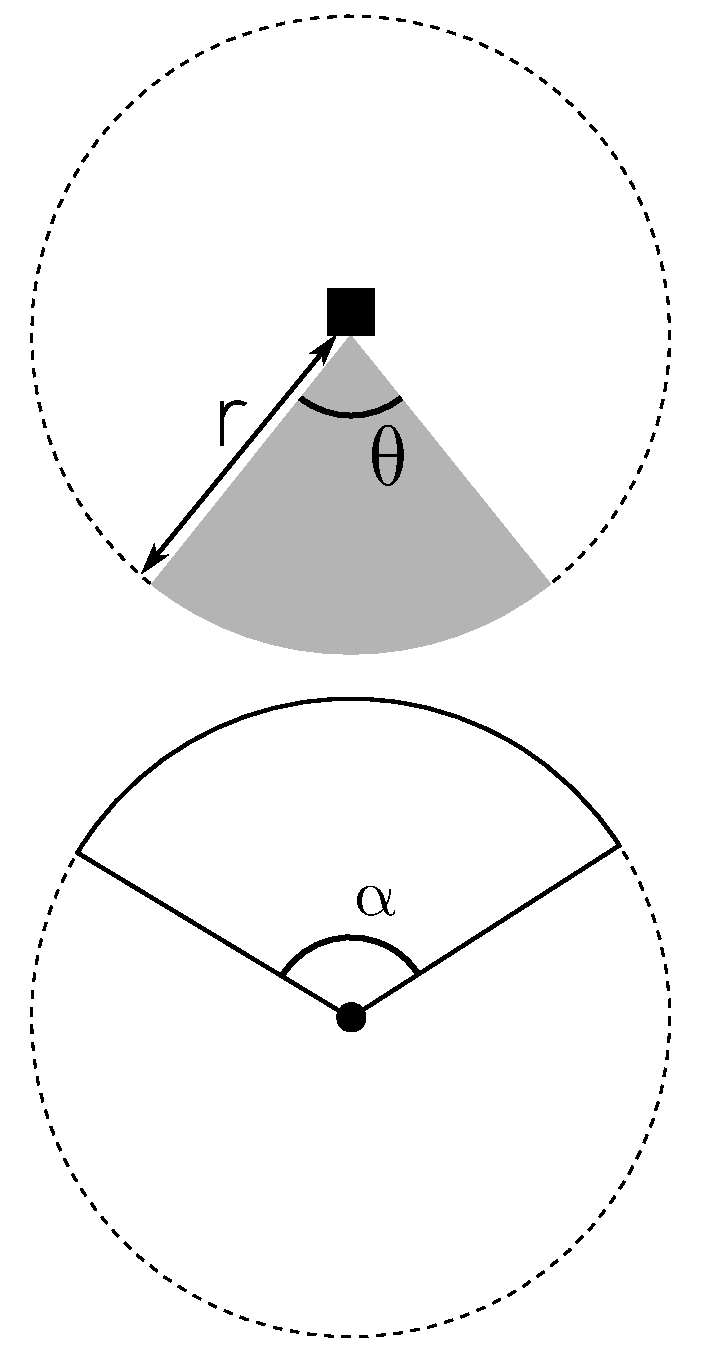
\includegraphics[width=4cm]{imgs/lucas_et_al_figure1.pdf}

\caption[Representation of sensor detection width and animal signal width]{
Representation of sensor detection width and animal signal width.
The filled square and circle represent a sensor and an animal, respectively; $\theta$, sensor detection width (radians); $r$, sensor detection distance; dark grey shaded area, sensor detection zone; $\alpha$, animal signal width (radians).
Dashed lines around the filled square and circle represents the maximum extent of $\theta$ and $\alpha$, respectively.} 
\label{f:AngleDef}
\end{figure}



\subsubsection{Gas Model}

Following \cite{yapp1956theory}, we derive the gas model where sensors can capture animals in any direction and animal signals are detectable from any direction ($\theta =  2\pi$ and $ \alpha =  2\pi$).
We assume that animals are in a homogeneous environment, and move in straight lines of random direction with velocity $v$.
We allow that our stationary sensor can capture animals at a detection distance $r$ and that if an animal moves within this detection zone they are captured with a probability of one; while outside this zone, animals are never captured.

In order to derive animal density, we need to consider relative velocity from the reference frame of the animals.
Conceptually, this requires us to imagine that all animals are stationary and randomly distributed in space, while the sensor moves with velocity $v$.
If we calculate the area covered by the sensor during the survey period, we can estimate the number of animals the sensor should capture.
As a circle moving across a plane, the area covered by the sensor per unit time is $2rv$.
The expected number of captures, $z$, for a survey period of $t$, with an animal density of $D$ is $z = 2rvtD$.
To estimate the density we rearrange to get $D = z/2rvt$.
Note that as $z$ is the number of encounters, not individuals, the possibility of repeated detections of the same individual is accounted for \cite{Hutchinson_Waser_2007}.


\subsubsection{gREM derivations for different detection and signal widths}
Different combinations of $\theta$ and $\alpha$ would be expected to occur (e.g., sensors have different detection widths and animals have different signal widths).
For different combinations $\theta$ and $\alpha$, the area covered per unit time is no longer given by $2rv$.
Instead of the size of the sensor detection zone having a diameter of $2r$, the size changes with the approach angle between the sensor and the animal.
The width of the area within which an animal can be detected is called the profile, $p$.
The size of $p$ depends on the signal width, detector width and the angle that the animal approaches the sensor.
The size of the profile (averaged across all approach angles) is defined as the average profile $\bar{p}$.
However, different combinations of $\theta$ and $\alpha$ need different equations to calculate $\bar{p}$. 




\begin{knitrout}\footnotesize
\definecolor{shadecolor}{rgb}{0.969, 0.969, 0.969}\color{fgcolor}\begin{figure}[t]

{\centering 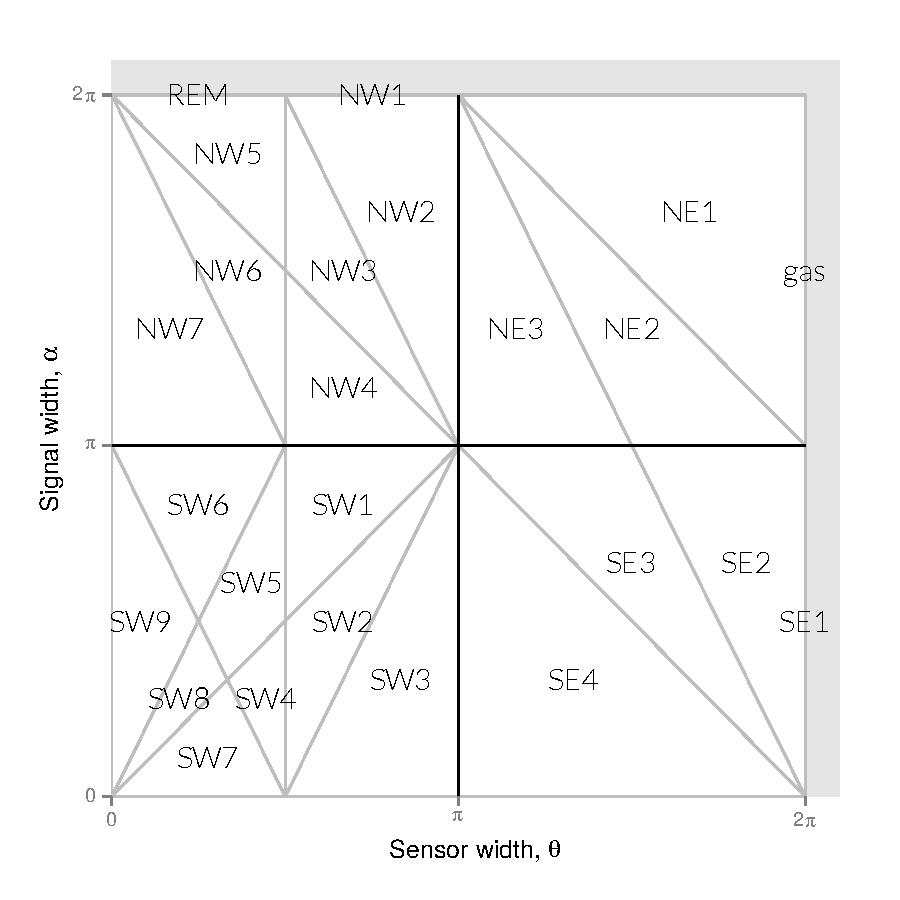
\includegraphics[width=0.6\textwidth]{figure/equalRegions-1} 

}

\caption[Locations where derivation of the average profile $\bar{p}$ is the same]{
Locations where derivation of the average profile $\bar{p}$ is the same for different combinations of sensor detection and animal signal widths.
Symbols within each polygon refer to each gREM submodel named after their compass point, except for Gas and REM which highlight the position of these previously derived models within the gREM.
Symbols on the edge of the plot are for submodels where $\alpha, \theta = 2\pi$
}\label{fig:equalRegions}
\end{figure}


\end{knitrout}

%\begin{figure}
%\centering
%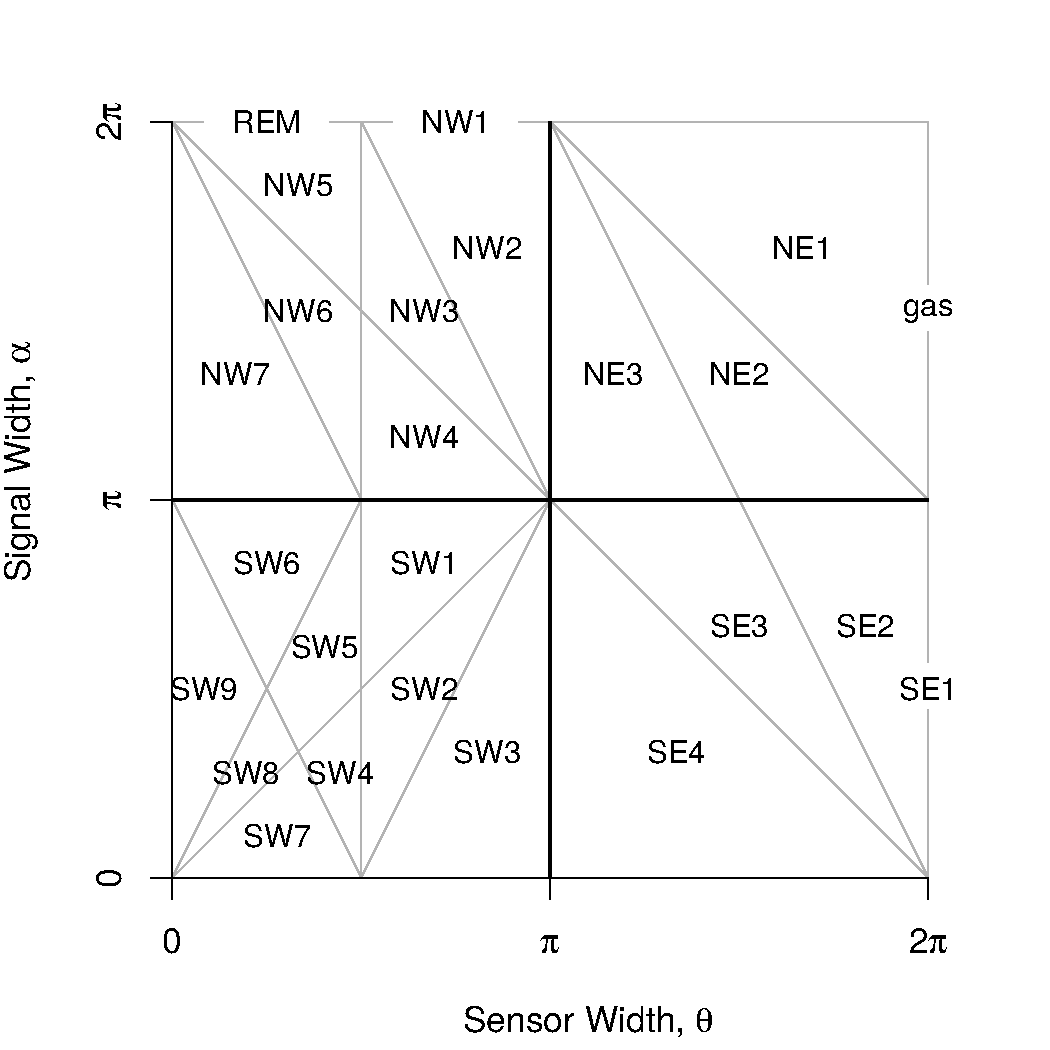
\includegraphics[width=7cm]{imgs/lucas_et_al_figure2.pdf}
%\caption[Locations where derivation of the average profile $\bar{p}$ is the same]{
%Locations where derivation of the average profile $\bar{p}$ is the same for different combinations of sensor detection and animal signal widths.
%Symbols within each polygon refer to each gREM submodel named after their compass point, except for Gas and REM which highlight the position of these previously derived models within the gREM.
%Symbols on the edge of the plot are for submodels where $\alpha, \theta = 2\pi$}
%\label{f:equalRegions}
%\end{figure}

We have identified the parameter space for the combinations of $\theta$ and $\alpha$ for which the derivation of the equations are the same (defined as sub-models in the gREM) (Figure~\ref{fig:equalRegions}).
For example, the gas model becomes the simplest gREM sub-model (upper right in Figure~\ref{fig:equalRegions}) and the REM from \cite{rowcliffe2008estimating} is another gREM sub-model where $\theta<\pi/2$ and $\alpha = 2\pi$.
We derive one gREM sub-model SE2 as an example below, where $2 \pi - \alpha/2 < \theta < 2\pi ,\; 0 < \alpha <\pi$ (see Appendix S2 for derivations of all gREM sub-models).
Any estimate of density would require prior knowledge of animal velocity, $v$ and animal signal width, $\alpha$ taken from other sources, for example existing literature \cite{brinklov2011, carbone2005far}.
Sensor width, $\theta$, and detection distance, $r$ would also need to be measured or obtained from manufacturer specifications \cite{holderied2003echolocation, adams2012you}.


\subsubsection{Example derivation of SE2}

In order to calculate $\bar{p}$, we have to integrate over the focal angle, $x_1$ (Figure~\ref{f:x1AndInt}a).
This is the angle taken from the centre line of the sensor.
Other focal angles are possible ($x_2$, $x_3$, $x_4$) and are used in other gREM sub-models (see Appendix S2).
As the size of the profile depends on the approach angle, we present the derivation across all approach angles.
When the sensor is directly approaching the animal $x_1  = \pi/2$.

Starting from $x_1 = \pi/2$ until $\theta/2 + \pi/2 - \alpha/2$, the size of the profile is $2r\sin \alpha/2$ (Figure~\ref{f:x1AndInt}b).
During this first interval, the size of $\alpha$ limits the width of the profile.
When the animal reaches $x_1$  = $\theta/2 + \pi/2 - \alpha/2$ (Figure~\ref{f:x1AndInt}c), the size of the profile is $r\sin( \alpha/2) + r\cos( x_1  - \theta/2)$ and the size of $\theta$ and $\alpha$ both limit the width of the profile (Figure~ \ref{f:x1AndInt}c).
Finally, at $x_1  = 5\pi/2 - \theta/2  - \alpha/2$ until $x_1  = 3\pi/2$, the width of the profile is again $2r\sin\alpha/2$ (Figure~ \ref{f:x1AndInt}d) and the size of $\alpha$ again limits the width of the profile. 


\begin{figure}[t]
	\centering
	\subfloat[\label{f:intx1}]{
		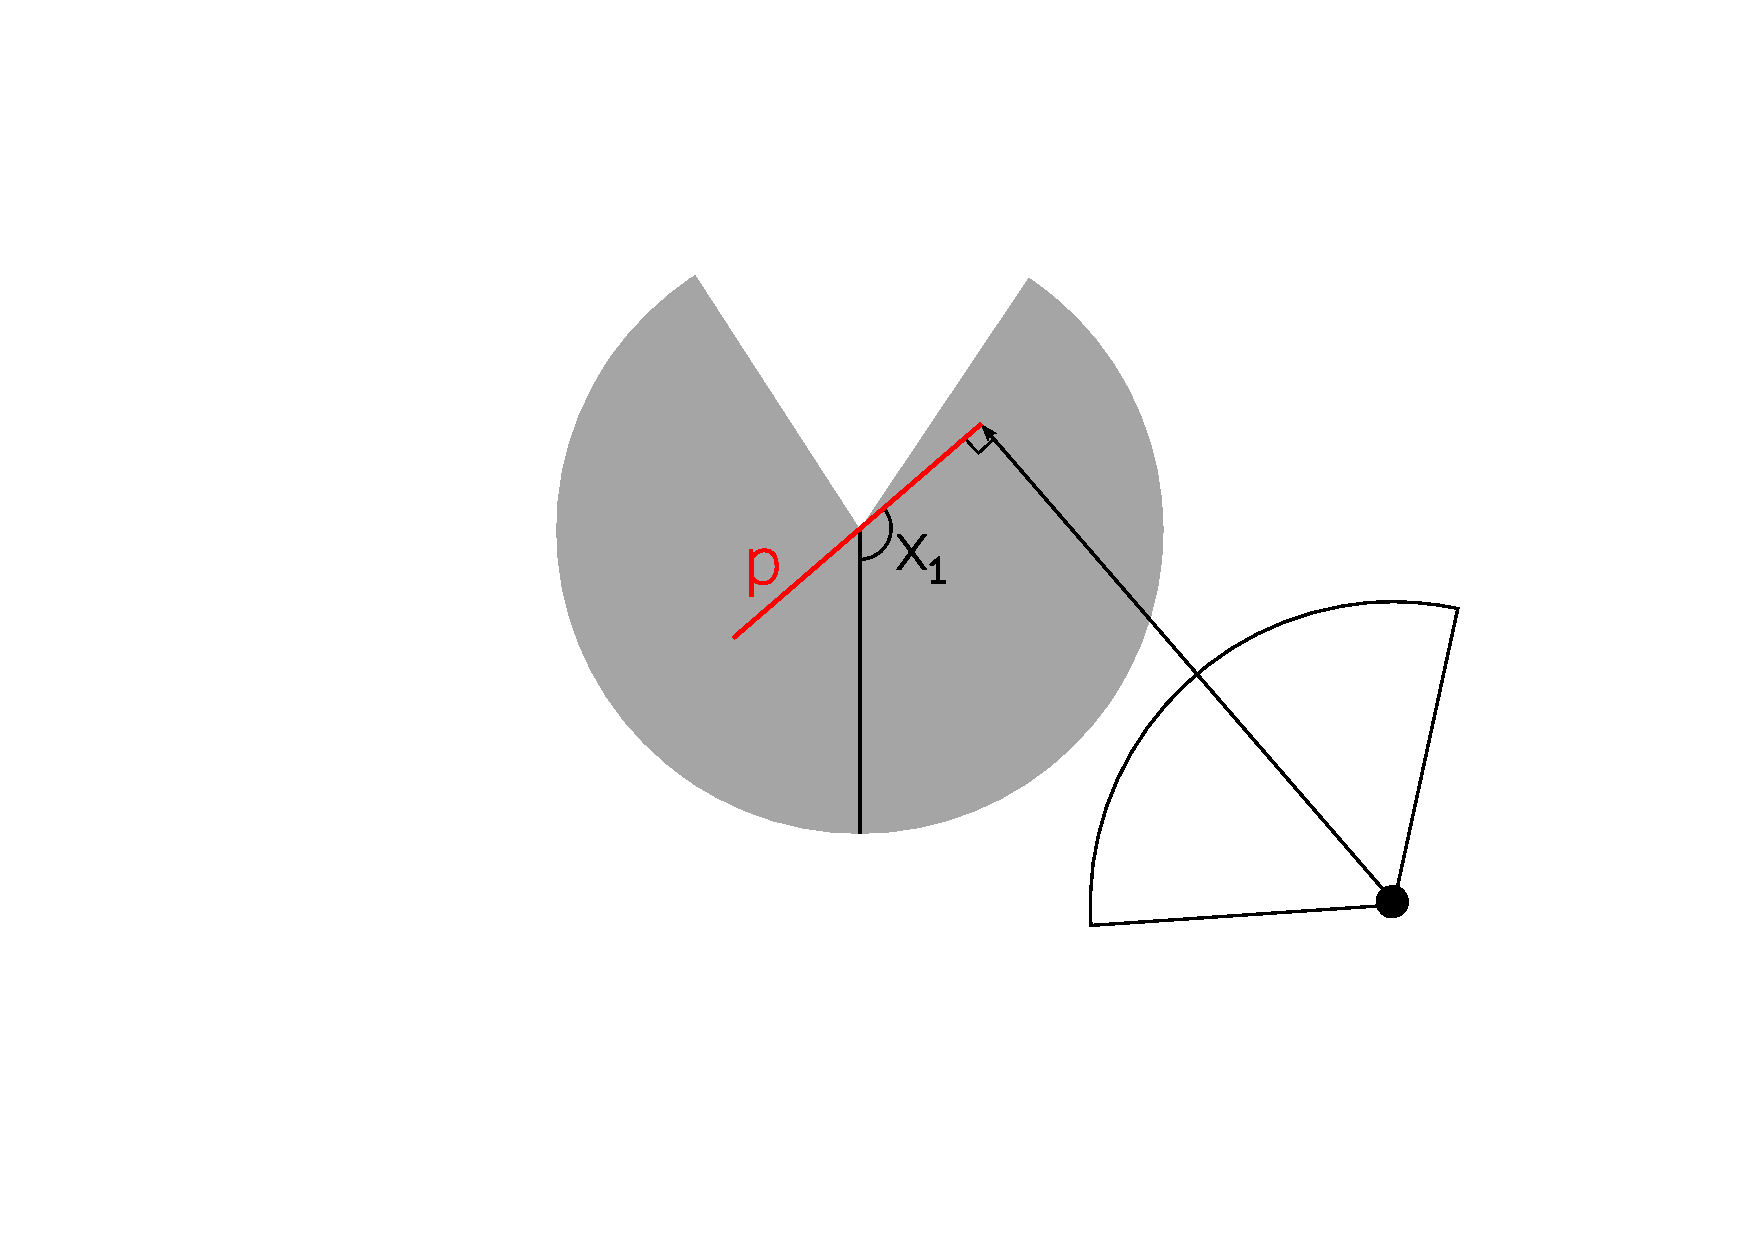
\includegraphics[trim = 20mm 40mm 20mm 10mm, width=70mm]{imgs/x1.pdf}
  }
  \subfloat[\label{f:int1}]{
		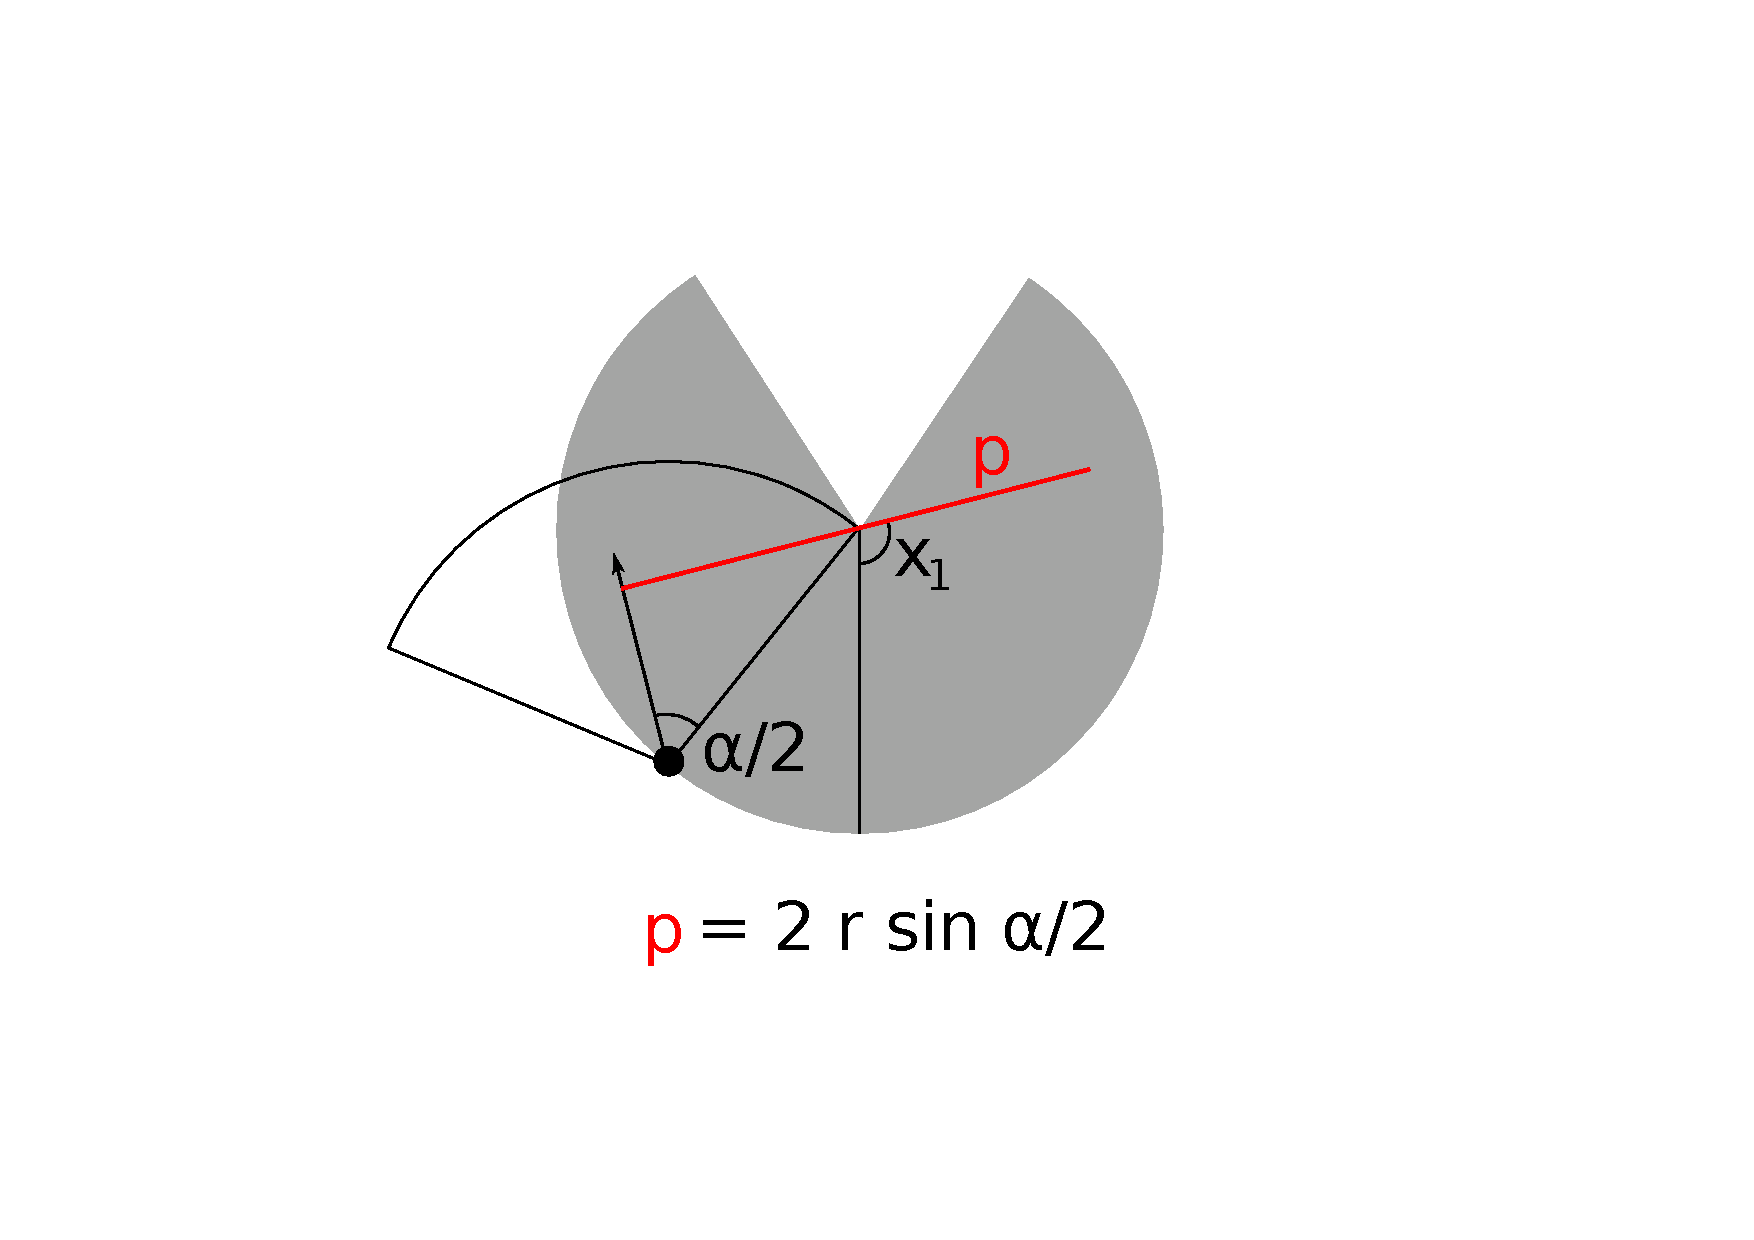
\includegraphics[trim = 20mm 40mm 20mm 10mm, width=70mm]{imgs/firstIntegral.pdf}
  }
  
  \subfloat[\label{f:int2}]{
		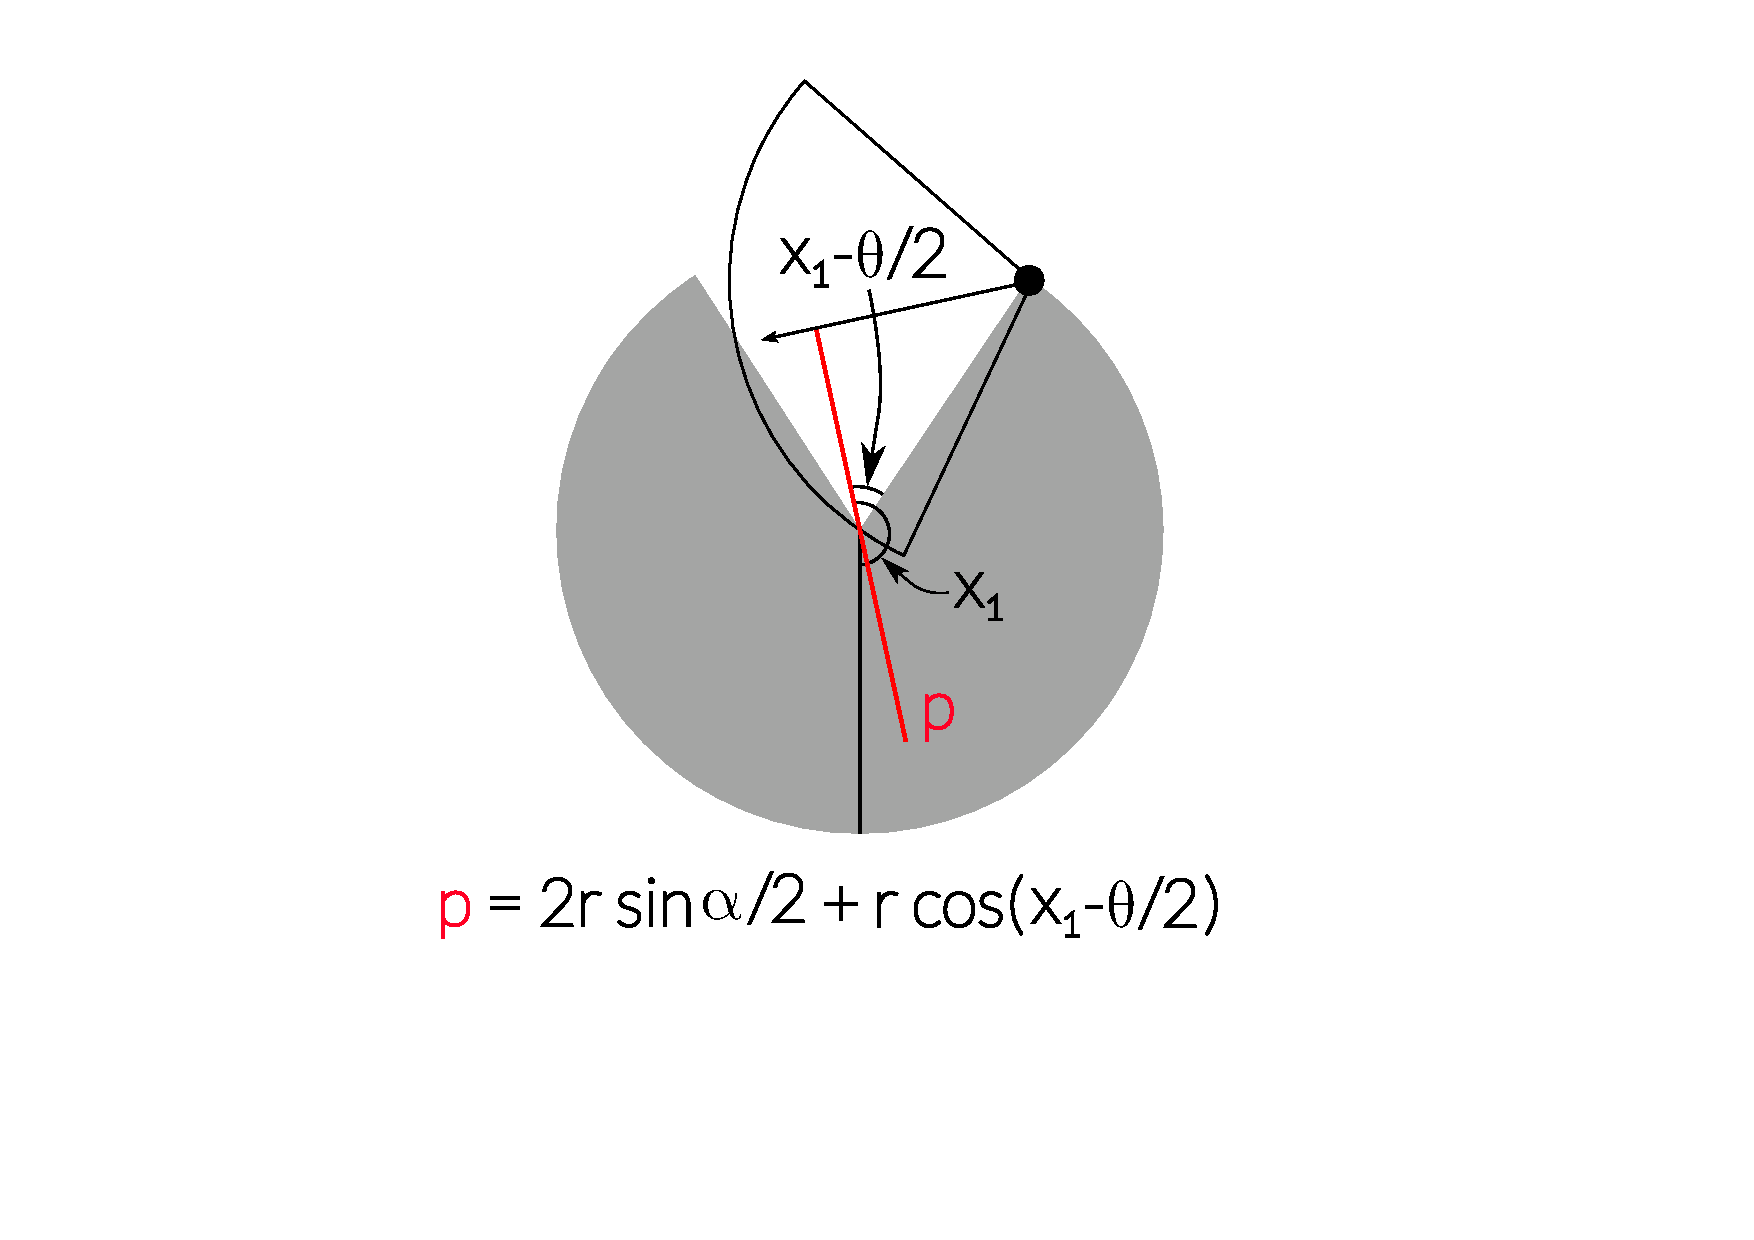
\includegraphics[trim = 20mm 40mm 20mm 10mm, width=70mm]{imgs/secondIntegral.pdf}
  }
  \subfloat[\label{f:int3}]{
		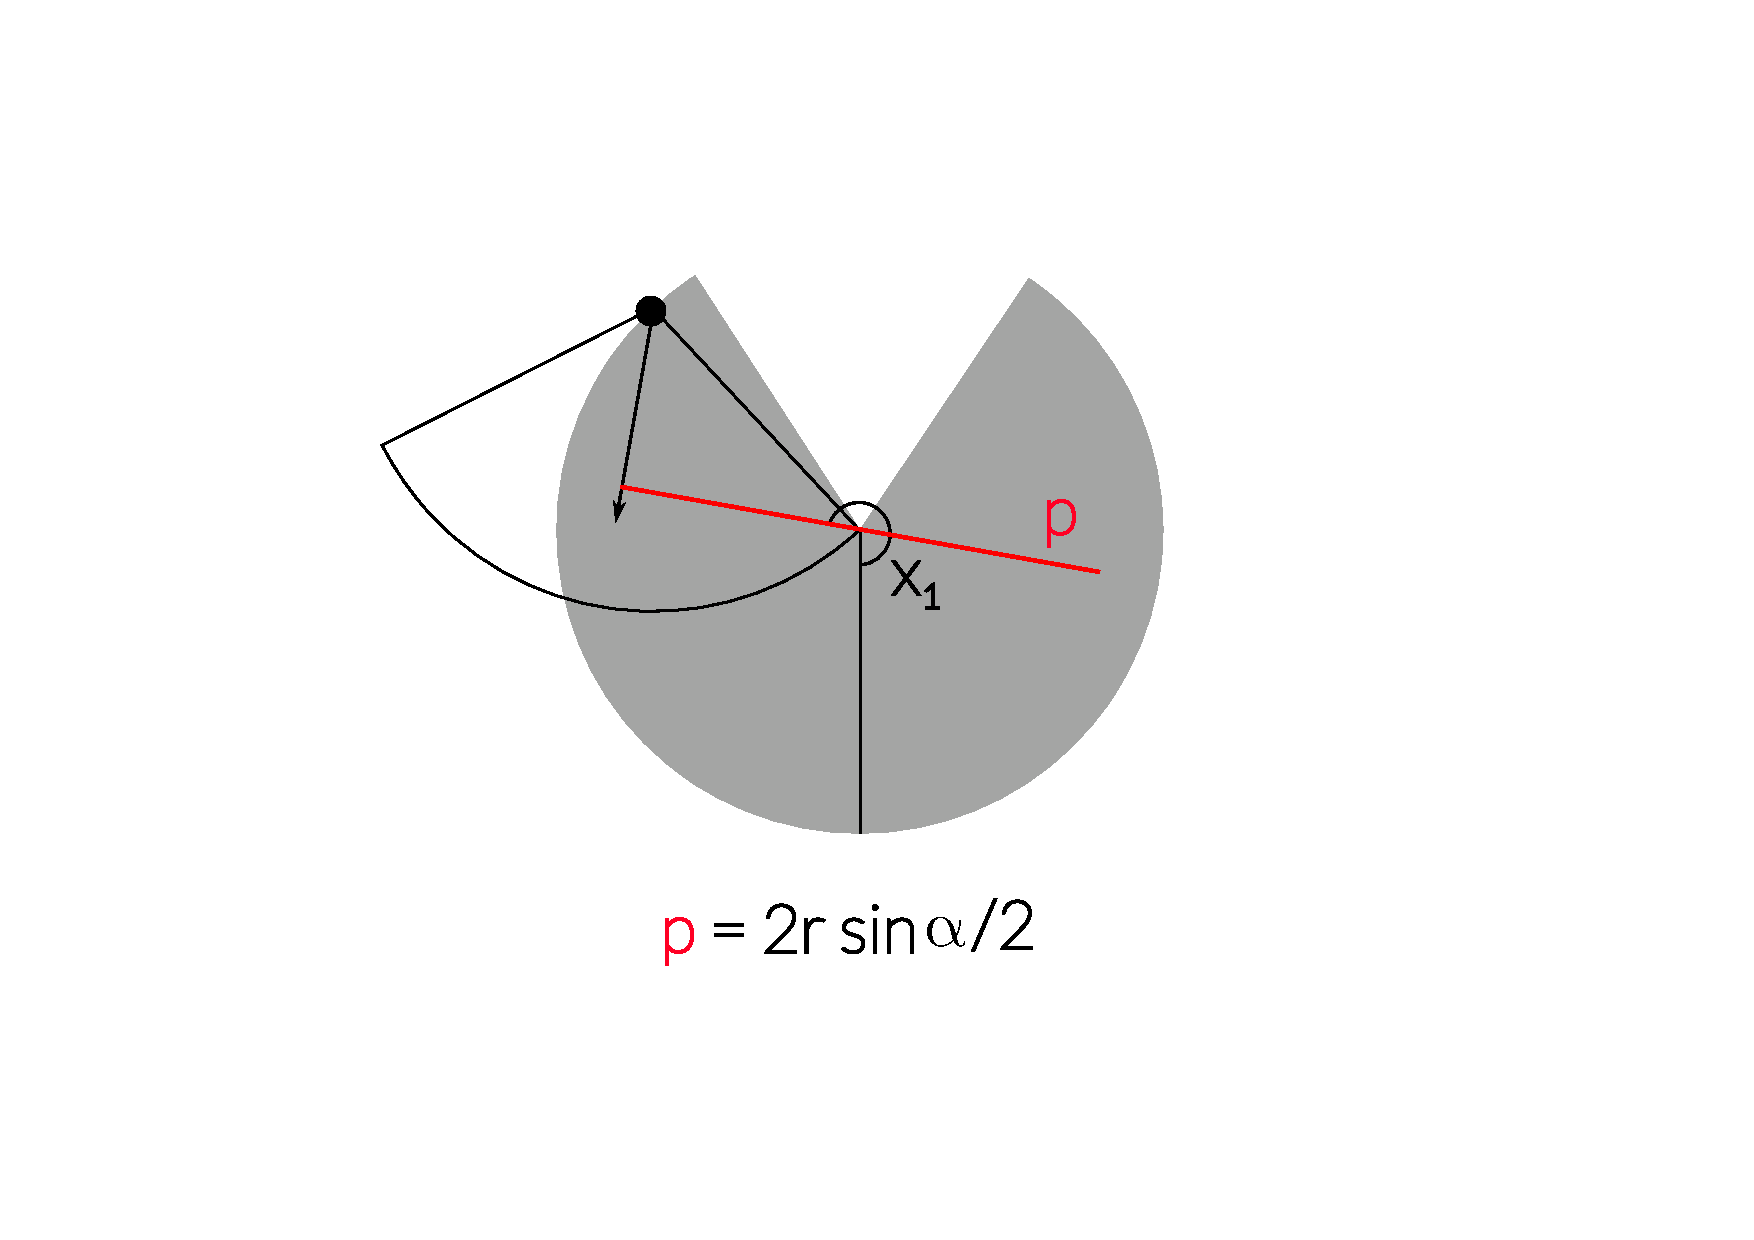
\includegraphics[trim = 20mm 40mm 20mm 10mm, width=70mm]{imgs/thirdIntegral.pdf}
  }

	%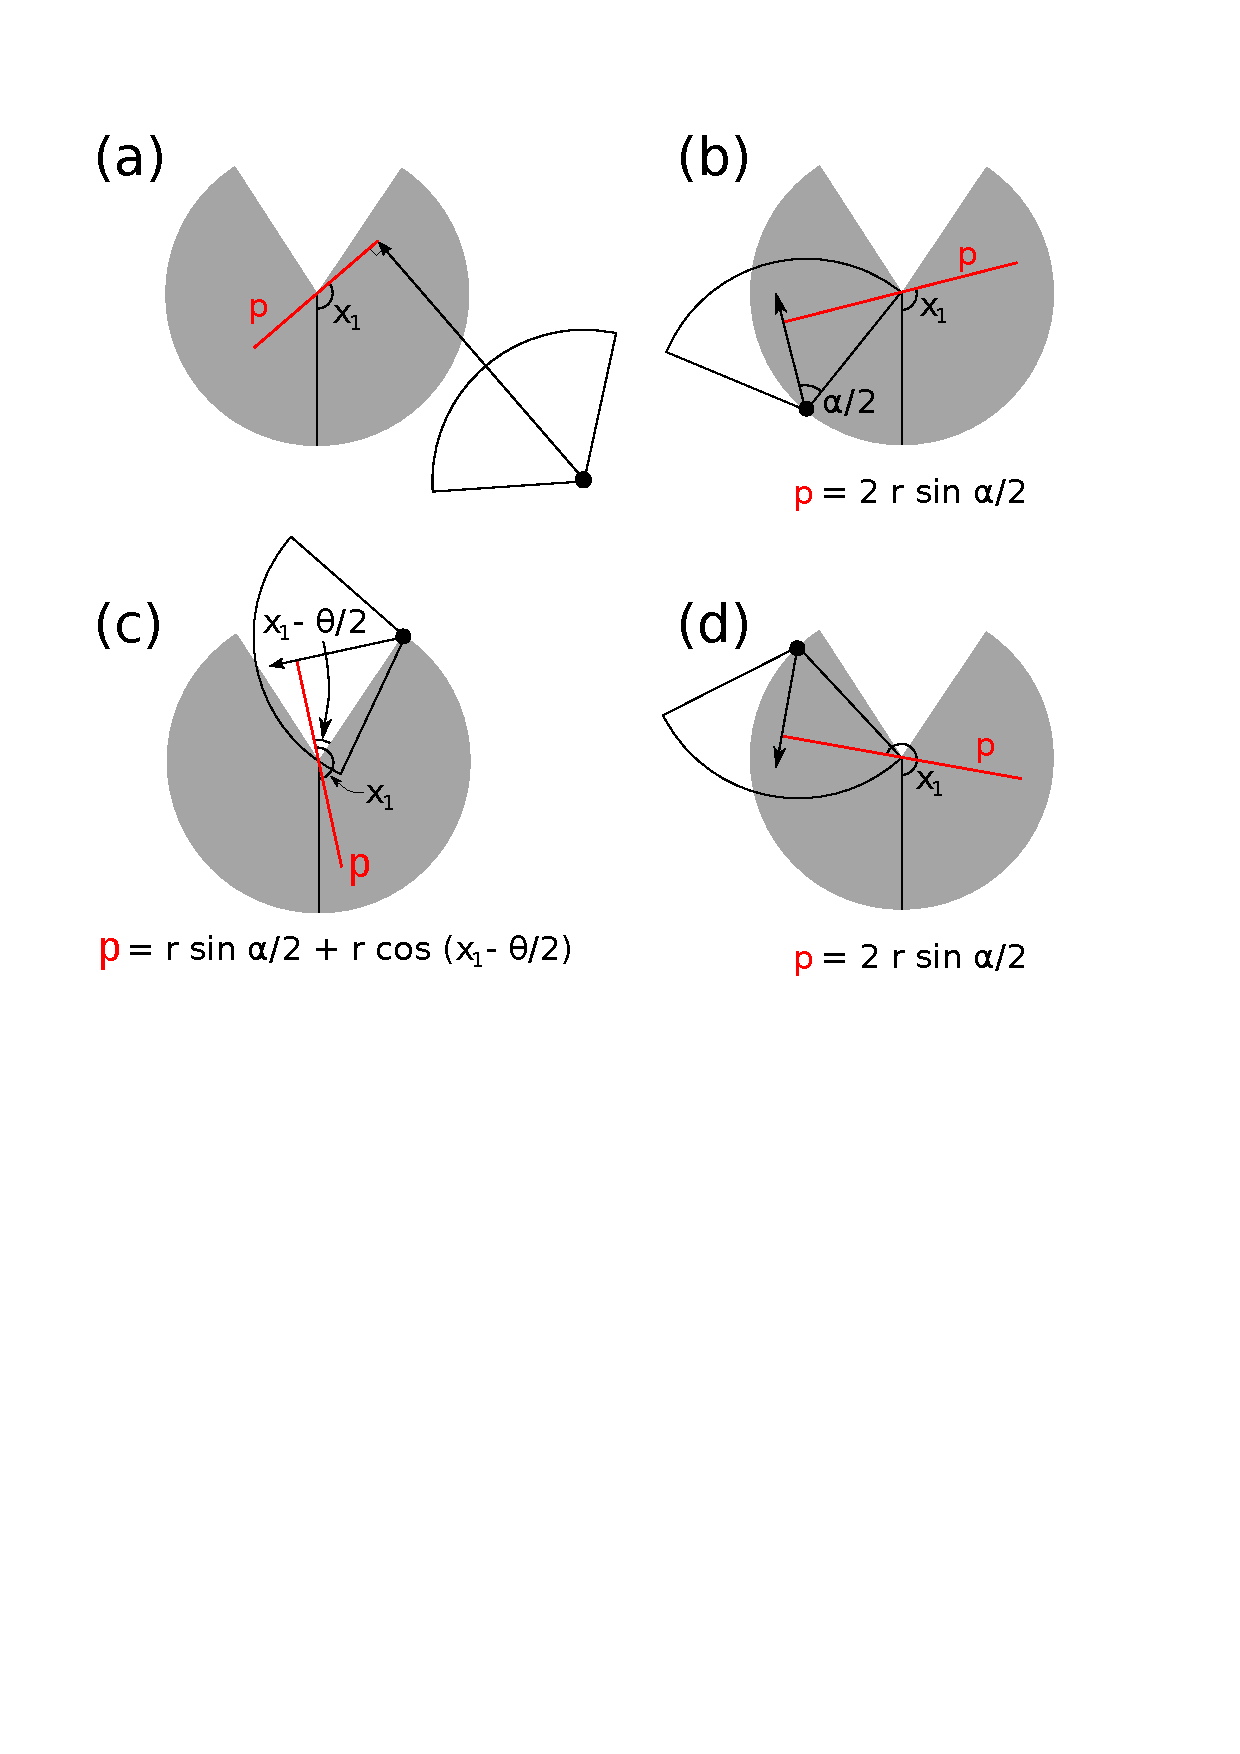
\includegraphics[width=7cm]{imgs/lucas_et_al_figure3.pdf}
\caption[An overview of the derivation of the average profile $\bar{p}$ for the gREM submodel SE2]{
An overview of the derivation of the average profile $\bar{p}$ for the gREM submodel SE2, where (a) shows the location of the profile $p$ (the line an animal must pass through in order to be captured) in red and the focal angle, $x_1$, for an animal (filled circle), its signal (unfilled sector), and direction of movement (shown as an arrow).
The detection zone of the sensor is shown as a filled grey sector with a detection distance of $r$.
The vertical black line within the circle shows the direction the sensor is facing.
The derivation of $p$ changes as the animal approaches the sensor from different directions (shown in b-d), where (b) is the derivation of $p$ when $x_1$ is in the interval $\lbrack\frac{\pi}{2}, \frac{\pi}{2} + \frac{\theta}{2} - \frac{\alpha}{2}\rbrack$, (c)  $p$ when $x_1$ is in the interval $\lbrack\frac{\pi}{2} + \frac{\theta}{2} - \frac{\alpha}{2}, \frac{5 \pi}{2} - \frac{\theta}{2} - \frac{\alpha}{2} \rbrack$ and (d) $p$ when $x_1$ is in the interval $\lbrack\frac{5 \pi}{2} - \frac{\theta}{2} - \frac{\alpha}{2}, \frac{3 \pi}{2}\rbrack$, where $\theta$, sensor detection width; $\alpha$, animal signal width.
The resultant equation for $p$ is shown beneath b-d.
The average profile $\bar{p}$ is the size of the profile averaged across all approach angles.}
\label{f:x1AndInt}

\end{figure}

The profile width $p$ for $\pi$ radians of rotation (from directly towards the sensor to directly behind the sensor) is completely characterised by the three intervals (Figure \ref{f:x1AndInt}b--d).
Average profile width $\bar{p}$ is calculated by integrating these profiles over their appropriate intervals of $x_1$ and dividing by $\pi$ which gives

\begin{align}
    \bar{p} &=\frac{1}{\pi} \left(\int\limits_{\frac{\pi}{2}}^{\frac{\pi}{2} + \frac{\theta}{2} - \frac{\alpha}{2}}2 r \sin{\frac{\alpha}{2} }\;\mathrm{d}x_1+\int\limits_{\frac{\pi}{2} + \frac{\theta}{2} - \frac{\alpha}{2}}^{\frac{5 \pi}{2} - \frac{\theta}{2} - \frac{\alpha}{2}}r \sin{\frac{\alpha}{2} } + r \cos{\left (x_1 - \frac{\theta}{2} \right )}\;\mathrm{d}x_1\right.\notag\\
 &\left.+\int\limits_{\frac{5 \pi}{2} - \frac{\theta}{2} - \frac{\alpha}{2}}^{\frac{3 \pi}{2}}2 r \sin{\frac{\alpha}{2} }\;\mathrm{d}x_1\right) \label{e:SE2int}  \\
     &= \frac{r}{\pi} \left(\theta \sin{\frac{\alpha}{2} } - \cos{\frac{\alpha}{2} } + \cos{\left (\frac{\alpha}{2} + \theta \right )}\right) \label{e:SE2result}
\end{align}

We then use this expression to calculate density
\begin{equation}
\label{e:gas}
D = z/vt\bar{p}.
\end{equation}


Rather than having one equation that describes $\bar{p}$ globally, the gREM must be split into submodels due to discontinuous changes in $p$ as $\alpha$ and $\beta$ change.
These discontinuities can occur for a number of reasons such as a profile switching between being limited by $\alpha$ and $\theta$, the difference between very small profiles and profiles of size zero, and the fact that the width of a sector stops increasing once the central angle reaches $\pi$ radians (i.e., a semi-circle is just as wide as a full circle).
As an example, if $\alpha$ is small, there is an interval between Figure \ref{f:x1AndInt}c and \ref{f:x1AndInt}d where the `blind spot' would prevent animals being detected giving $p=0$.
This would require an extra integral in our equation, as simply putting our small value of $\alpha$ into \ref{e:SE2int} would not give us this integral of $p=0$.

gREM submodel specifications were done by hand, and the integration was done using SymPy \cite{sympy} in Python (Appendix S3).
The gREM submodels were checked by confirming that: (1) submodels adjacent in parameter space were equal at the boundary between them; (2) submodels that border $ \alpha = 0$ had $p = 0$ when $ \alpha = 0$; (3) average profile widths $\bar{p}$ were between 0 and $2r$ and; (4) each integral, divided by the range of angles that it was integrated over, was between 0 and $2r$.
The scripts for these tests are included in Appendix S3 and the R \cite{R} implementation of the gREM is given in Appendix S4.  

\subsection{Simulation Model}

We tested the accuracy and precision of the gREM by developing a spatially explicit simulation of the interaction of sensors and animals using different combinations of sensor detection widths, animal signal widths, number of captures, and models of animal movement.
One hundred simulations were run where each consisted of a  \SI{7.5}{\kilo\meter} by \SI{7.5}{\kilo\meter} square with periodic boundaries.
A stationary sensor of radius $r$, \SI{10}{\meter}, was set up in the exact centre of each simulated study area, covering seven sensor detection widths $\theta$, between 0 and $2\pi$ ($2/9\pi$, $4/9\pi$, $6/9\pi$, $8/9\pi$, $10/9\pi$, $14/9\pi$, and $2\pi$).
Each sensor was set to record continuously and to capture animal signals instantaneously from emission.
Each simulation was populated with a density of \SI{70}{\animals\per\kilo\meter\squared}, calculated from the equation in \cite{damuth1981population} as the expected density of mammals weighing \SI{1}{\gram}.
This density therefore represents a reasonable estimate of density of individuals, given that the smallest mammal is around \SI{2}{\gram} \cite{jones2009pantheria}.
A total of 3937 individuals per simulation were created which were placed randomly at the start of the simulation. 11 signal widths $\alpha$ between 0 and $\pi$ were used ($1/11\pi$, $2/11\pi$, $3/11\pi$, $4/11\pi$, $5/11\pi$, $6/11\pi$, $7/11\pi$, $8/11\pi$, $9/11\pi$, $10/11\pi$, $\pi$). 

Each simulation lasted for $N$ steps (14400) of duration $T$ (15 minutes) giving a total duration of 150 days.
The individuals moved within each step with a distance $d$, with an average speed, $v$.
The distance, $d$, was sampled from a normal distribution with mean distance, $\mu_d = vT$, and standard deviation, $\sigma_d = vT/10$, where the standard deviation was chosen to scale with the average distance travelled.
An average speed, $v = $ \SI{40}{\kilo\meter \per \day}, was chosen based on the largest day range of terrestrial animals \cite{carbone2005far}, and represents the upper limit of realistic speeds.
At the end of each step, individuals were allowed to either remain stationary for a time step (with a given probability, $S$), or change direction where the change in direction has a uniform distribution in the interval $\left[-A, A\right]$.
This resulted in seven different movement models where: (1) simple movement, where $S$ and $A$ = 0; (2) stop-start movement, where (i) $S$ = 0.25, $A$ = 0, (ii) $S$ = 0.5, $A$ = 0, (iii) $S$ = 0.75, $A$ = 0; (3) correlated random walk movement, where (i) $S$ = 0, $A$ = $\pi/3$, (ii) $S$ = 0, $A$ = $2\pi/3$, iii) $S$ = 0, $A$ = $\pi$.
Individuals were counted as they moved into the detection zone of the sensor per simulation. 

We calculated the estimated animal density from the gREM by summing the number of captures per simulation and inputting these values into the correct gREM submodel.
The accuracy of the gREM was determined by comparing the true simulation density with the estimated density.
Precision of the gREM was determined by the standard deviation of estimated densities.
We used this method to compare the accuracy and precision of all the gREM submodels.
As these submodels are derived for different combinations of $\alpha$ and $\theta$, the accuracy and precision of the submodels was used to determine the impact of different values of $\alpha$ and $\theta$. 

The influence of the number of captures and animal movement models on accuracy and precision was investigated using four different gREM submodels representative of the range $\alpha$ and $\theta$ values (submodels NW1, SW1, NE1, and SE3, Figure~\ref{fig:equalRegions}).
From a random starting point we ran the simulation until a range of different capture numbers were recorded (from 10 to 100 captures), recorded the length of time this took, and estimated the animal density for each of the four sub-models.
These estimated densities were compared to the true density to assess the impact on the accuracy and precision of the gREM.
We calculated the coefficient of variation in order to compare the precision of the density estimates from simulations with different expected numbers of captures.
The gREM also assumes that individuals move continuously with straight-line movement (simple movement model) and we therefore assessed the impact of breaking the gREM assumptions.
We used the four submodels to compare the accuracy and precision of a simple movement model, stop-start movement models (using different average amounts of time spent stationary), and random walk movement models.
Finally, as the parameters ($\alpha$, $\beta$, $r$ and $v$) are likely to be measured with error, we compared true simulation densities to densities estimated with parameters with errors of $0\%$, $\pm 5\%$ and $\pm 10\%$, for all gREM submodels.


\section{Results}

\subsection{Analytical model}

The equation for $\bar{p}$ has been newly derived for each submodel in the gREM, except for the gas model and REM which have been calculated previously.
However, many models, although derived separately, have the same expression for $\bar{p}$.
Figure~\ref{f:equalModelResults} shows the expression for $\bar{p}$ in each case.
The general equation for density, \ref{e:gas}, is used with the correct value of $\bar{p}$ substituted.
Although more thorough checks are performed in Appendix S3, it can be seen that all adjacent expressions in Figure~\ref{f:equalModelResults} are equal when expressions for the boundaries between them are substituted in.






\begin{figure}
	\centering
	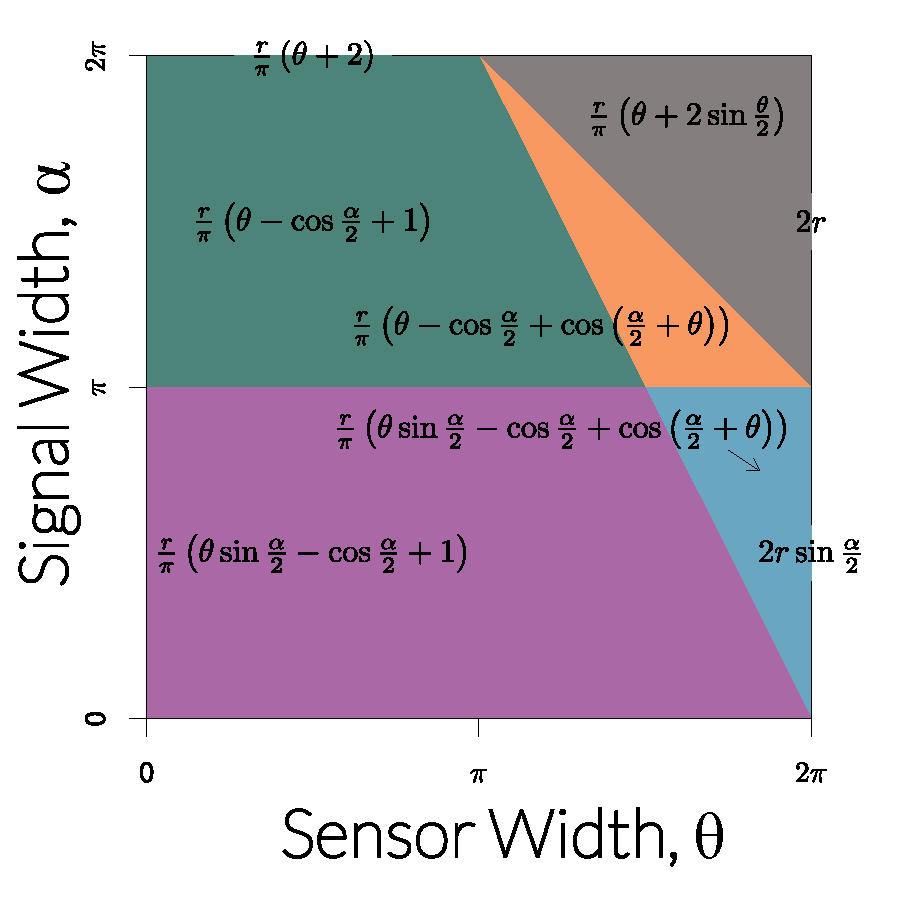
\includegraphics[width=7cm]{imgs/equalRegionsExpressions.pdf}
	\caption[Expressions for the average profile width]{
Expressions for the average profile width, $\bar{p}$, given a range of sensor and signal widths.
Despite independent derivation within each block, many models result in the same expression.
These are collected together and presented as one block of colour.
Expressions on the edge of the plot are for submodels with $\alpha, \theta = 2\pi$. }
	\label{f:equalModelResults}
\end{figure}


\subsection{Simulation model}

\subsubsection{gREM submodels}
All gREM submodels showed a high accuracy, i.e., the median difference between the estimated and true values was less than 2\% across all models (Figure~\ref{fig:gremSubmods}).
However, the precision of the submodels do vary, where the gas model is the most precise and the SW7 sub model the least precise, having the smallest and the largest interquartile range, respectively (Figure~\ref{fig:gremSubmods}).
The standard deviation of the error between the estimated and true densities is strongly related to both the sensor and signal widths (Appendix S5), such that larger widths have lower standard deviations (greater precision) due to the increased capture rate of these models.



\begin{knitrout}\footnotesize
\definecolor{shadecolor}{rgb}{0.969, 0.969, 0.969}\color{fgcolor}\begin{figure}[t]

{\centering 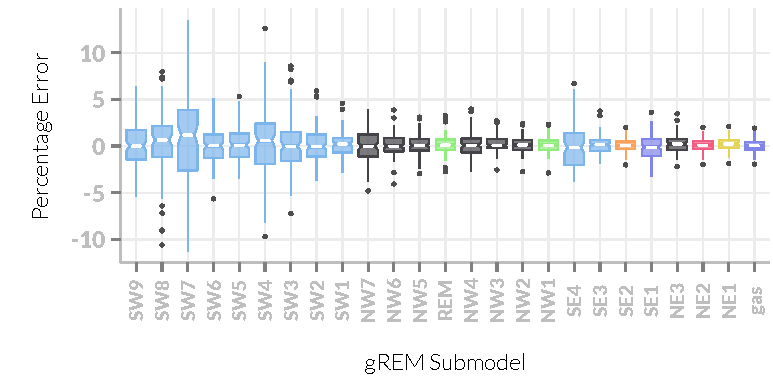
\includegraphics[width=\textwidth]{figure/gremSubmods-1} 

}

\caption[Simulation model results of the accuracy and precision for gREM submodels]{
Simulation model results of the accuracy and precision for gREM submodels.
The percentage error between estimated and true density for each gREM sub model is shown within each box plot, where the white line represents the median percentage error across all simulations, boxes represent the middle 50\% of the data, whiskers represent variability outside the upper and lower quartiles with outliers plotted as individual points.
Notches indicate 95\% confidence intervals.
Box colours correspond to the expressions for average profile width $\bar{p}$ given in Figure \ref{f:equalModelResults}. 
}\label{fig:gremSubmods}
\end{figure}


\end{knitrout}

%\begin{figure}[t]
%	\centering
%	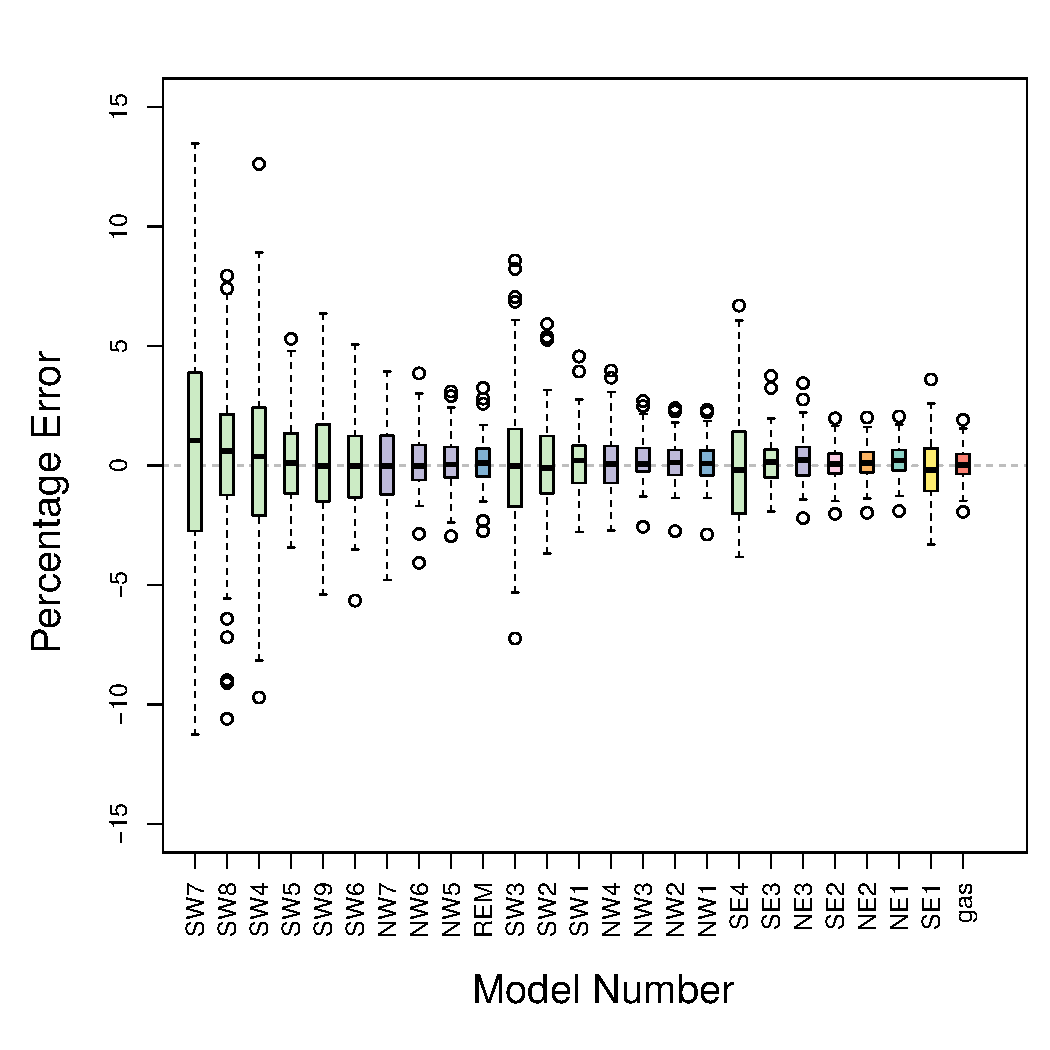
\includegraphics[width=7cm]{imgs/lucas_et_al_figure5.pdf}
%       	\caption[Simulation model results of the accuracy and precision for gREM submodels]{Simulation model results of the accuracy and precision for gREM submodels.
%The percentage error between estimated and true density for each gREM sub model is shown within each box plot, where the black line represents the median percentage error across all simulations, boxes represent the middle 50\% of the data, whiskers represent variability outside the upper and lower quartiles with outliers plotted as individual points.
%Box colours correspond to the expressions for average profile width $\bar{p}$ given in Figure 4.        
%} 
%	\label{f:ModelBias}
%\end{figure}

\subsubsection{Number of captures}

Within the four gREM submodels tested (NW1, SW1, SE3, NE1), the accuracy was not strongly affected by the number of captures.
The median difference between the estimated and true values was less than 15\% across all capture rates (Figure~\ref{fig:Captures}).
However, the precision was dependent on the number of captures across all four of the gREM submodels, where precision increases as number of captures increases, as would be expected for any statistical estimate (Figure~\ref{fig:Captures}).
For all gREM submodels, the the coefficient of variation falls to 10\% at 100 captures. 



\begin{knitrout}\footnotesize
\definecolor{shadecolor}{rgb}{0.969, 0.969, 0.969}\color{fgcolor}\begin{figure}[t]

{\centering 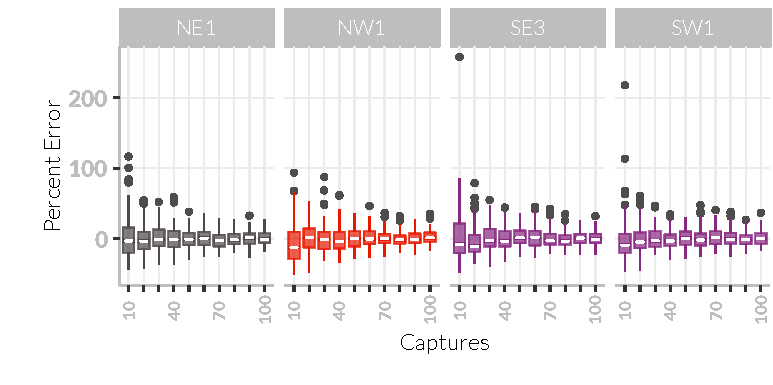
\includegraphics[width=0.8\textwidth]{figure/Captures-1} 

}

\caption[Simulation model results of the accuracy and precision of four gREM submodels]{
Simulation model results of the accuracy and precision of four gREM submodels (NW1, SW1, SE3 and NE1) given different numbers of captures.
The percentage error between estimated and true density within each gREM sub model for capture rate is shown within each box plot, where the white line represents the median percentage error across all simulations, boxes represent the middle 50\% of the data, whiskers represent variability outside the upper and lower quartiles with outliers plotted as individual points.
Notches show the 95\% confidence interval.
Sensor and signal widths vary between submodels.
The numbers beneath each plot represent the coefficient of variation.
The colour of each box plot corresponds to the expressions for average profile width $\bar{p}$ given in Figure \ref{f:equalModelResults}. 
}\label{fig:Captures}
\end{figure}


\end{knitrout}

%\begin{figure}[t]
%  \centering
%	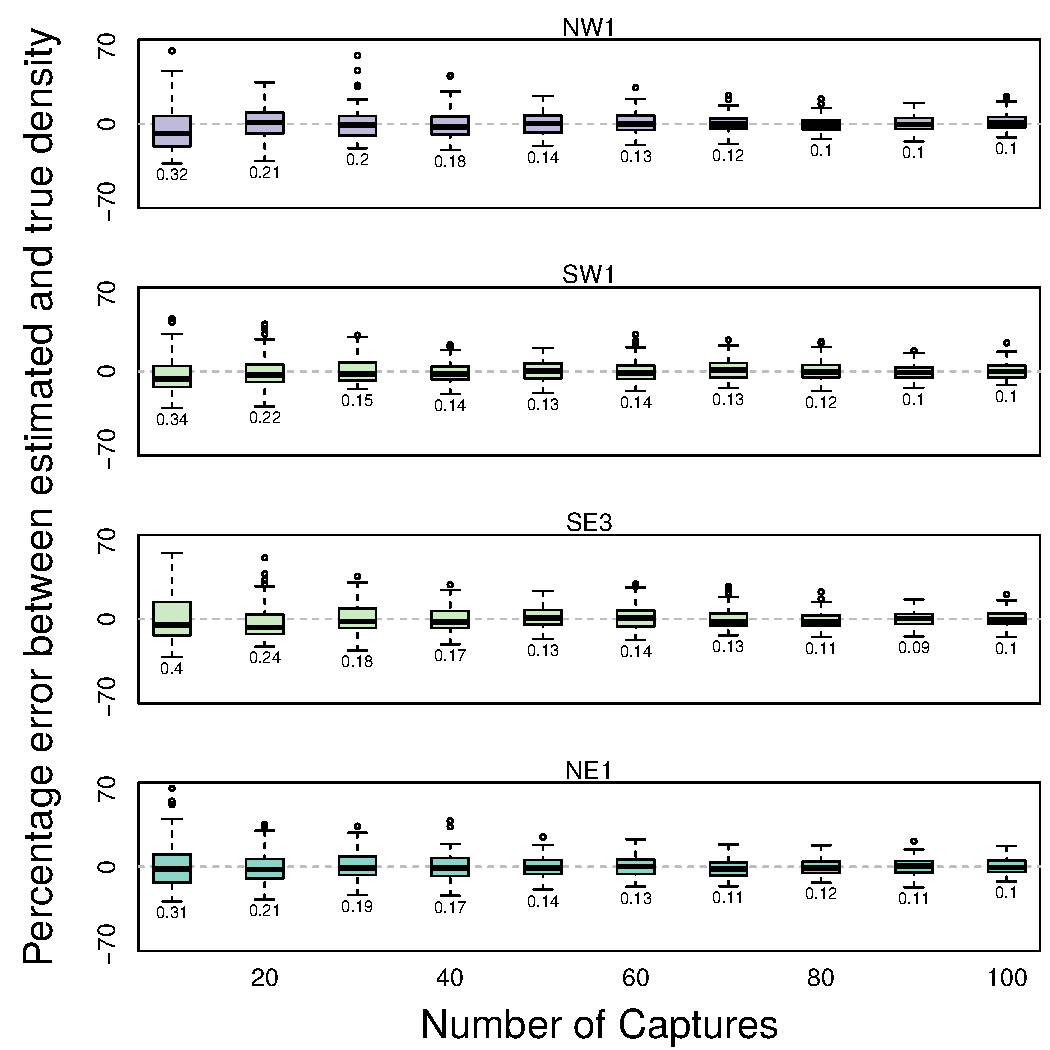
\includegraphics[width=7cm]{imgs/lucas_et_al_figure6.pdf}
%\caption[Simulation model results of the accuracy and precision of four gREM submodels]{
%Simulation model results of the accuracy and precision of four gREM submodels (NW1, SW1, SE3 and NE1) given different numbers of captures.
%The percentage error between estimated and true density within each gREM sub model for capture rate is shown within each box plot, where the black line represents the median percentage error across all simulations, boxes represent the middle 50\% of the data, whiskers represent variability outside the upper and lower quartiles with outliers plotted as individual points.
%Sensor and signal widths vary between submodels.
%The numbers beneath each plot represent the coefficient of variation.
%The colour of each box plot corresponds to the expressions for average profile width $\bar{p}$ given in Figure 4. }            
%\label{f:Captures}
%\end{figure}

\subsubsection{Movement models}

Within the four gREM submodels tested (NW1, SW1, SE3, NE1), neither the accuracy or precision was affected by the average amount of time spent stationary.
The median difference between the estimated and true values was less than 2\% for each category of stationary time (0, 0.25, 0.5 and 0.75) (Figure~\ref{fig:movtFig}).
Altering the maximum change in direction in each step (0, $\pi/3$, $2\pi/3$, and $\pi$) did not affect the accuracy or precision of the four gREM submodels (Figure~\ref{fig:movtFig}). 

\subsubsection{Impact of parameter error}

The percentage error in the density estimates across all parameters and gREM submodels shows a similar response for under and over estimated parameters, suggesting the accuracy is reasonable with respect to parameter error (Appendix S6).
The impact of parameter error on the precision of the density estimate varies across gREM submodels and parameters, where $\alpha$ shows the largest variation including the largest values.
However, in all cases the percentage error in the density estimate is not more than 5\% greater than the error in the parameter estimate (Appendix S6).



\begin{knitrout}\footnotesize
\definecolor{shadecolor}{rgb}{0.969, 0.969, 0.969}\color{fgcolor}\begin{figure}[t]

{\centering 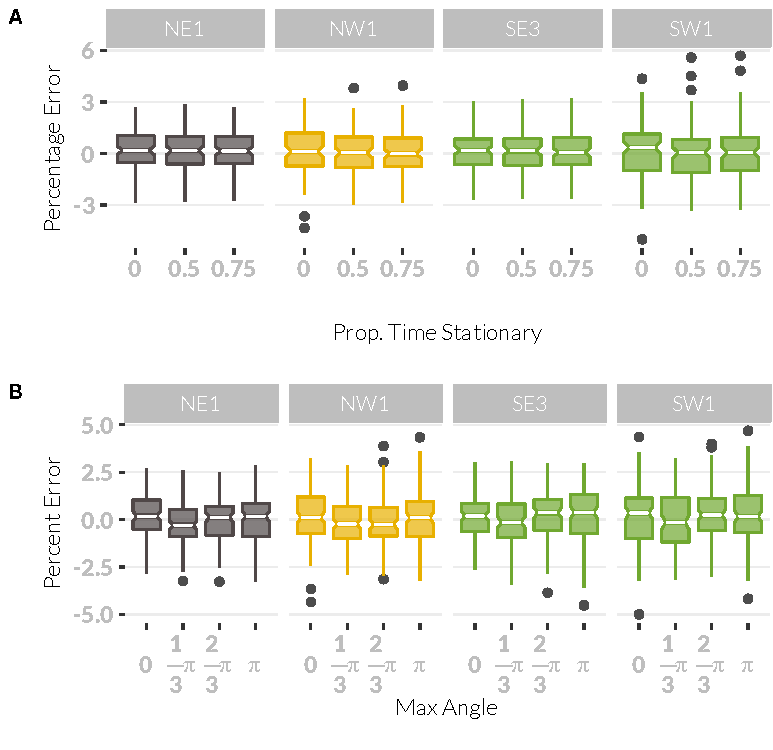
\includegraphics[width=0.7\textwidth]{figure/movtFig-1} 

}

\caption[Simulation model results of the accuracy and precision of four gREM submodels]{
Simulation model results of the accuracy and precision of four gREM submodels (NW1, SW1, SE3 and NE1) given different movement models where (a) average amount of time spent stationary (stop-start movement) and (b) maximum change in direction at each step (correlated random walk model).
The percentage error between estimated and true density within each gREM sub model for the different movement models is shown within each box plot, where the white line represents the median percentage error across all simulations, boxes represent the middle 50\% of the data, whiskers represent variability outside the upper and lower quartiles with outliers plotted as individual points.
Notches in boxplots show the 95\% confidence for the median.
The simple model is represented where time and maximum change in direction equals 0.
The colour of each box plot corresponds to the expressions for average profile width $\bar{p}$ given in Figure 4.
}\label{fig:movtFig}
\end{figure}


\end{knitrout}

                  
%%%% ------- Discussion ---------%%%%
\section{Discussion}

\subsection{Analytical model}

We have developed the gREM such that it can be used to estimate density from acoustic sensors and camera traps.
This has entailed a generalisation of the gas model and the REM in \cite{rowcliffe2008estimating} to be applicable to any combination of sensor width  $\theta$ and signal directionality $\alpha$.
We emphasise that the approach is robust to multiple detections of the same individual.
We have used simulations to show, as a proof of principle, that these models are accurate and precise. 

There are a number of possible extensions to the gREM which could be developed in the future.
The original gas model was formulated for the case where both animals and sensor are moving \cite{Hutchinson_Waser_2007}.
Indeed any of the models which have animals that are equally detectable in all directions ($\alpha = 2\pi$) can be trivially expanded by replacing animal speed $v$ with $v + v_s$ where $v_s$ is the speed of the sensor.
However, when the animal has a directional call the extension becomes less simple.
The approach would be to calculate again the mean profile width.
However, for each angle of approach, one would have to average the profile width for an animal facing in any direction (i.e., not necessarily moving towards the sensor) weighted by the relative velocity of that direction.
There are a number of situations where a moving detector and animal could occur, e.g.
an acoustic detector towed from a boat when studying porpoises \cite{kimura2014acoustic} or surveying echolocating bats from a moving car \cite{jones2011indicator}. 

Interesting but unstudied problems impacting the gREM are firstly, edge effects caused by sensor trigger delays (the delay between sensing an animal and attempting to record the encounter) \cite{rovero2013camera}, and secondly, sensors which repeatedly turn on an off during sampling \cite{jones2011indicator}.
The second problem is particularly relevant to acoustic detectors which record ultrasound by time expansion.
Here ultrasound is recorded for a set time period and then slowed down and played back, rendering the sensor 'deaf' periodically during sampling.
Both of these problems may cause biases in the gREM, as animals can move through the detection zone without being detected.
As the gREM assumes constant surveillance, the error created by switching the sensor on and off quickly will become more important if the sensor is only on for short periods of time.
We recommend that the gREM is applied to constantly sampled data, and the impacts of breaking these assumptions on the gREM should be further explored. 

\subsection{Accuracy, Precision and Recommendations for Best Practice}
Based on our simulations, we believe that the gREM has the potential to produce accurate estimates for many different species, using either camera traps or acoustic detectors.
However, the precision of the gREM differed between submodels.
For example, when the sensor and signal width were small, the precision of the model was reduced.
Therefore when choosing a sensor for use in a gREM study, the sensor detection width should be maximised.
If the study species has a narrow signal directionality, other aspects of the study protocol, such as length of the survey, should be used to compensate. 

The precision of the gREM is greatly affected by the number of captures.
The coefficient of variation falls dramatically between 10 and 60 captures and then after this continues to slowly reduce.
At 100 captures the submodels reach 10\% coefficient of variation, considered to be a very good level of precision and better than many previous studies \cite{thomas2012passive, o2003crouching, foster2012critique}.  The length of surveys in the field will need to be adjusted so that enough data can be collected to reach this precision level.
Populations of fast moving animals or populations with high densities will require less survey effort than those species that are slow moving or have populations with low densities. 

We found that the sensitivity of the gREM to inaccurate parameter estimates was both predictable and reasonable (Appendix S6), although this varies between different parameters and gREM submodels.
Whilst care should be taken in parameter estimation when analysing both acoustic and camera trap data, acoustic data poses particular problems.
For acoustic surveys, estimates of $r$ (detection distance) can be measured directly or calculated using sound attenuation models \cite{holderied2003echolocation}, while the sensor angle is often easily measured \cite{adams2012you} or found in the manufacturer's specifications.
When estimating animal movement speed $v$, only the speed of movement during the survey period should be used.
The signal width is the most sensitive parameter to inaccurate estimates (Appendix S6) and is also the most difficult to measure.  While this parameter will typically be assumed to be $2\pi$ for camera trap surveys, fewer estimates exist for acoustic signal widths.
Although signal width has been measured for echolocating bats using arrays of microphones \cite{brinklov2011}, more work should be done on obtaining estimates for a range of acoustically surveyed species.



\subsection{Limitations}

Although the REM has been found to be effective in field tests \cite{rowcliffe2008estimating, zero2013monitoring}, the gREM requires further validation by both field tests and simulations.
For example, capture-mark-recapture methods could be used alongside the gREM to test the accuracy under field conditions \cite{rowcliffe2008estimating}.
While we found no effect of the movement model on the accuracy or precision of the gREM, the models we have used in our simulations to validate the gREM are still simple representations of true animal movement.
Animal movement may be highly nonlinear and often dependent on multiple factors such as behavioural state and existence of home ranges \cite{smouse2010stochastic}.
Therefore testing the gREM against real animal data, or further simulations with more complex movement models, would be beneficial.

The assumptions of our simulations may require further consideration, for example we have assumed an equal density across the study area.
However, in a field environment the situation may be more complex, with additional variation coming from local changes in density between sensor sites.
Athough unequal densities should theoretically not affect accuracy \cite{Hutchinson_Waser_2007}, it will affect precision and further simulations should be used to quantify this effect.
Additionally, we allowed the sensor to be stationary and continuously detecting, negating the triggering, and non-continuous recording issues that could exist with some sensors and reduce precision or accuracy.
Finally, in the simulation animals moved at the equivalent of the largest day range of terrestrial animals \cite{carbone2005far}.
Slower speed values should not alter the accuracy of the gREM, but precision would be affected since slower speeds produce fewer records.
The gREM was both accurate and precise for all the movement models we tested (stop-start movement and correlated random walks).

A feature of the gREM is that it does not fit a statistical model to estimate detection probability as occupancy models and distance sampling do \cite{royle2003estimating, barlow2005estimates, marques2011estimating}.
Instead it explicitly models the process, with animals only being detected if they approach the sensor from a suitable direction.
Other processes that affect detection probability could be included in the model to improve realism.

\subsection{Implications for ecology and conservation}

The gREM is applicable for count data obtained either visually or acoustically in both marine and terrestrial environments, and is suitable for taxa including echolocating bats \cite{walters2012continental}, songbirds \cite{buckland2006point}, whales \cite{marques2011estimating} and forest primates \cite{hassel2008reliable}.
Many of these taxa contain critically endangered species and monitoring their populations is of conservation interest.
For example, current methods of density estimation for the threatened Franciscana dolphin (\emph{Pontoporia blainvillei}) may result in underestimation of their numbers \cite{crespo2010abundance}.
In addition, using gREM may be easier than other methods for measuring the density of animals which may be useful in quantifying ecosystem services, such as songbirds with a known positive influence on pest control \cite{jirinec2011roosting}.

The gREM will aid researchers to study species with non-invasive methods such as remote sensors, which allows for large, continuous monitoring projects with limited human resources \cite{kelly2012noninvasive}.
The gREM is also suitable  for species that are sensitive to human contact or are difficult or dangerous to catch \cite{thomas2012passive}.
As sensors such as camera traps and acoustic detectors become more ubiquitous, the gREM will be increasingly useful for monitoring unmarked animal populations across broad spatial, temporal and taxonomic scales.


%%%% ------- Acknowledgments ---------%%%%
%\section{Acknowledgments}
%We thank Hilde Wilkinson-Herbot, Chris Carbone, Francois Balloux, Andrew Cunningham, Steve Hailes, Richard Glennie and an anonymous referee for comments on previous versions of the manuscript.
%This study was funded through CoMPLEX PhD studentships at University College London supported by BBSRC and EPSRC (EAM and TCDL) and The Darwin Initiative (Awards 15003, 161333, EIDPR075), NERC (NE/H525003/1), and The Leverhulme Trust (Philip Leverhulme Prize) for KEJ.

%%%% ------- Data Accessibility ---------%%%%
%\section{Data Accessibility}

%The code used in this chapter is available on Github at \url{https://github.com/timcdlucas/lucasMoorcroftManuscript/tree/postPeerReview}.







\section{Appendix}

  

\clearpage
\section{Table of symbols}

%move to appendix
\begin{table}[h!]
\centering
\begin{tabular}{lll}
Symbol 	& Description & Units\\\hline
$\theta$	& Sensor width & \SI{}{\radian} \\
$\alpha$	& Animal signal width & \SI{}{\radian} \\
$x_i$	        & Focal angle, $i \in \{1,2,3,4\} $ 	& \SI{}{\radian}\\
$r$ 		& Detection distance & \SI{}{\meter}\\
$\bar{p}$ 		& Average profile width & \SI{}{\meter}\\
$p$ 		& A specific profile width & \SI{}{\meter}\\
$v$		& Velocity & \SI{}{\meter\per\second}\\
$t$		& Time & \SI{}{\second}\\
$z$		& Number of detections & -\\
$D$		& Animal density & \SI{}{\per\meter\squared} \\
$T$ 		& Step length & \SI{}{\second}\\
$N$ 		& Number of steps per simulation & -\\
$d$ 		& Distance moved in a time step & \SI{}{\meter}\\
$S$ 		& Probability of remaining stationary & -\\
$A$ 		& Maximum turning angle & \SI{}{\radian}\\
\\
\end{tabular}
\caption{List of symbols used to describe the gREM and simulations. `-' means the quantity has no units.}
\label{t:paras}
\end{table}

\clearpage

\section{Supplementary Methods}
\subsection{Introduction}
\lettr{T}hese supplementary methods derive all the models used. 
For continuity, the gas model derivation is included here as well as in the main text. 
The calculation of all integrals use in the gREM is included in the Python script S3. 



\subsection{Gas model} \label{gas}

Following \cite{yapp1956theory}, we derive the gas model where sensors can capture animals in any direction and animal signals are detectable from any direction ($ \theta =  2\pi$ and $ \alpha =  2\pi$).
We assume that animals are in a homogeneous environment, and move in straight lines of random direction with velocity $v$.
We allow that our stationary sensor can capture animals at a detection distance $r$ and that if an animal moves within this detection zone they are captured with a probability of one, while animals outside the zone are never captured.




\begin{figure}[t]
  \centering
{
  \subfloat[$x_1$\label{fig:x1}]{
    \centering
    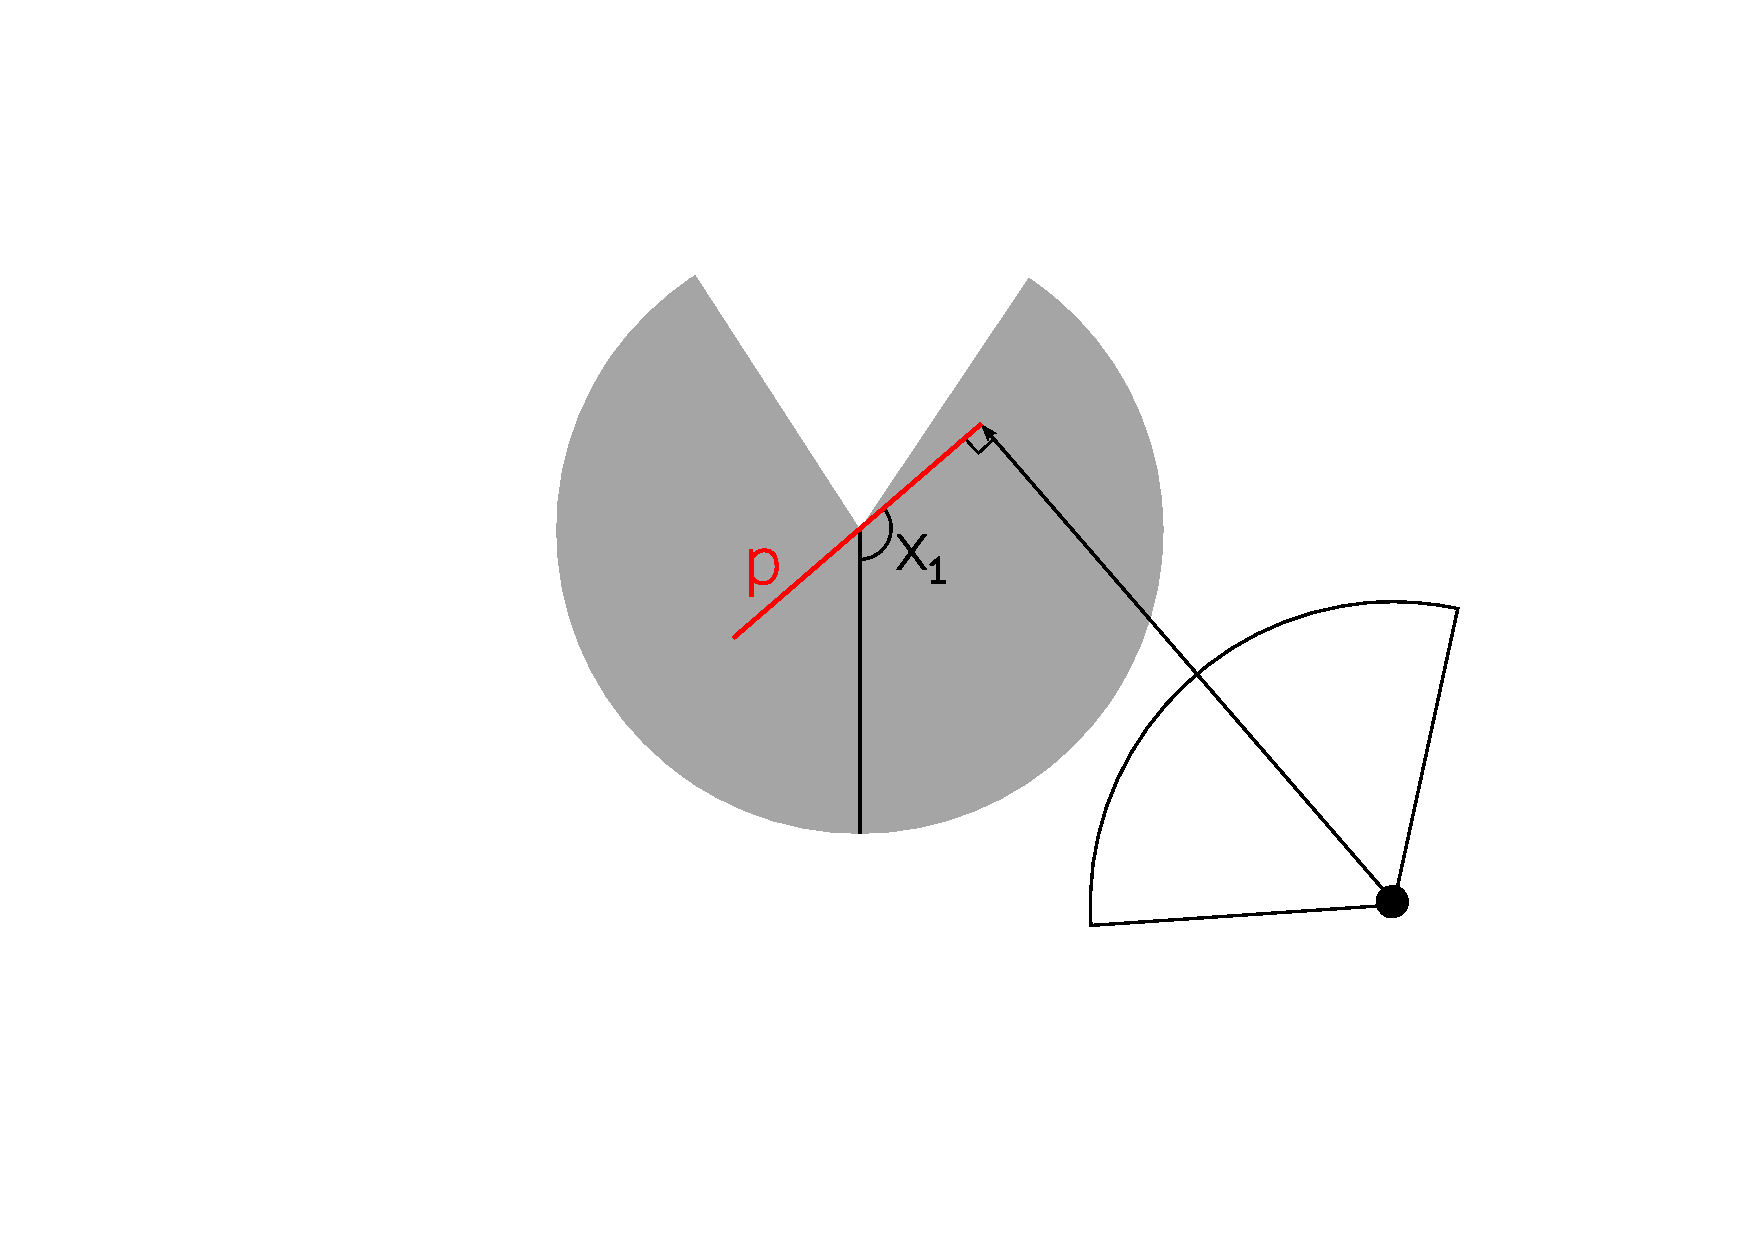
\includegraphics[width=.44\textwidth, trim=2cm 1cm 2cm 3cm]{imgs/x1.pdf}
  }
  \subfloat[$x_2$\label{fig:x2}]{
    \centering
    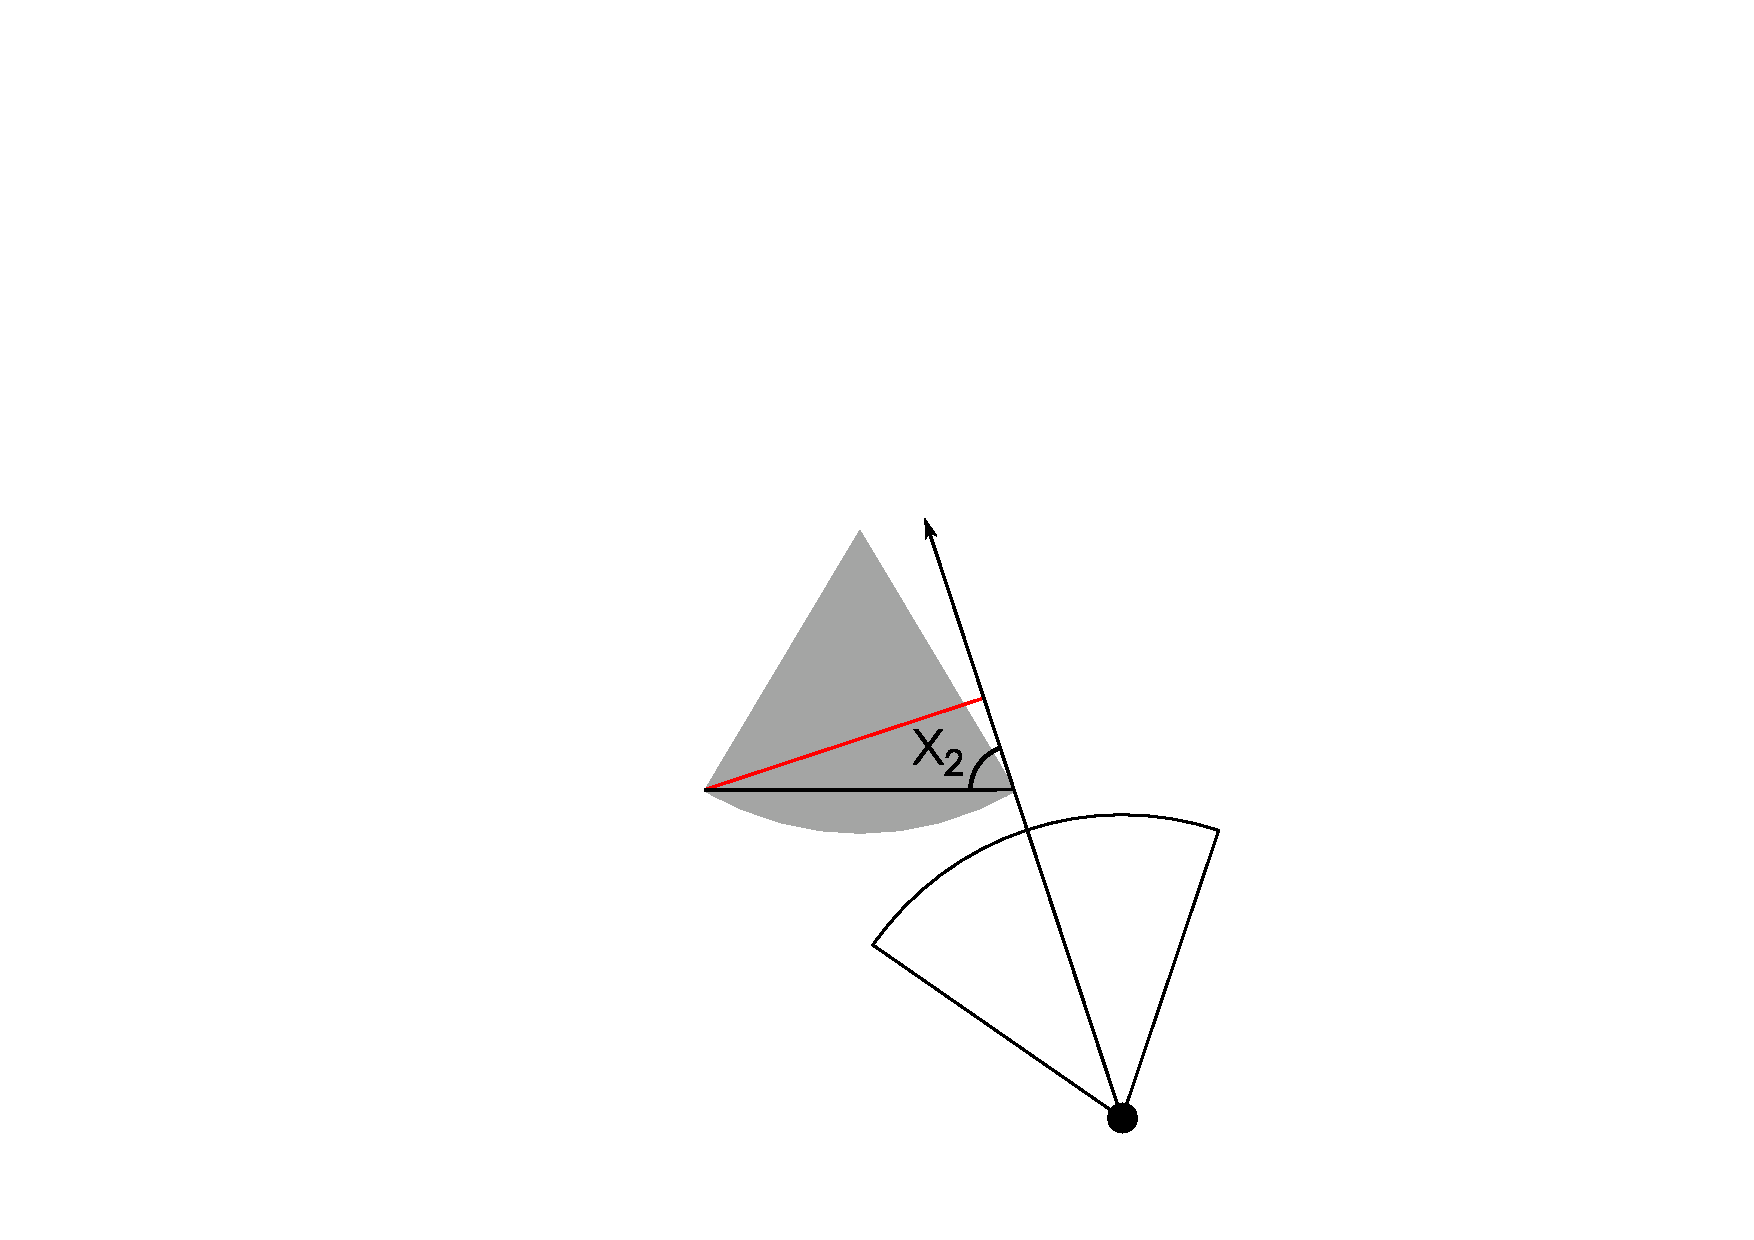
\includegraphics[width=.29\textwidth, trim=9cm 2cm 9cm 6cm]{imgs/x2.pdf}
  }
  
  \subfloat[$x_3$\label{fig:x3}]{
    \centering
    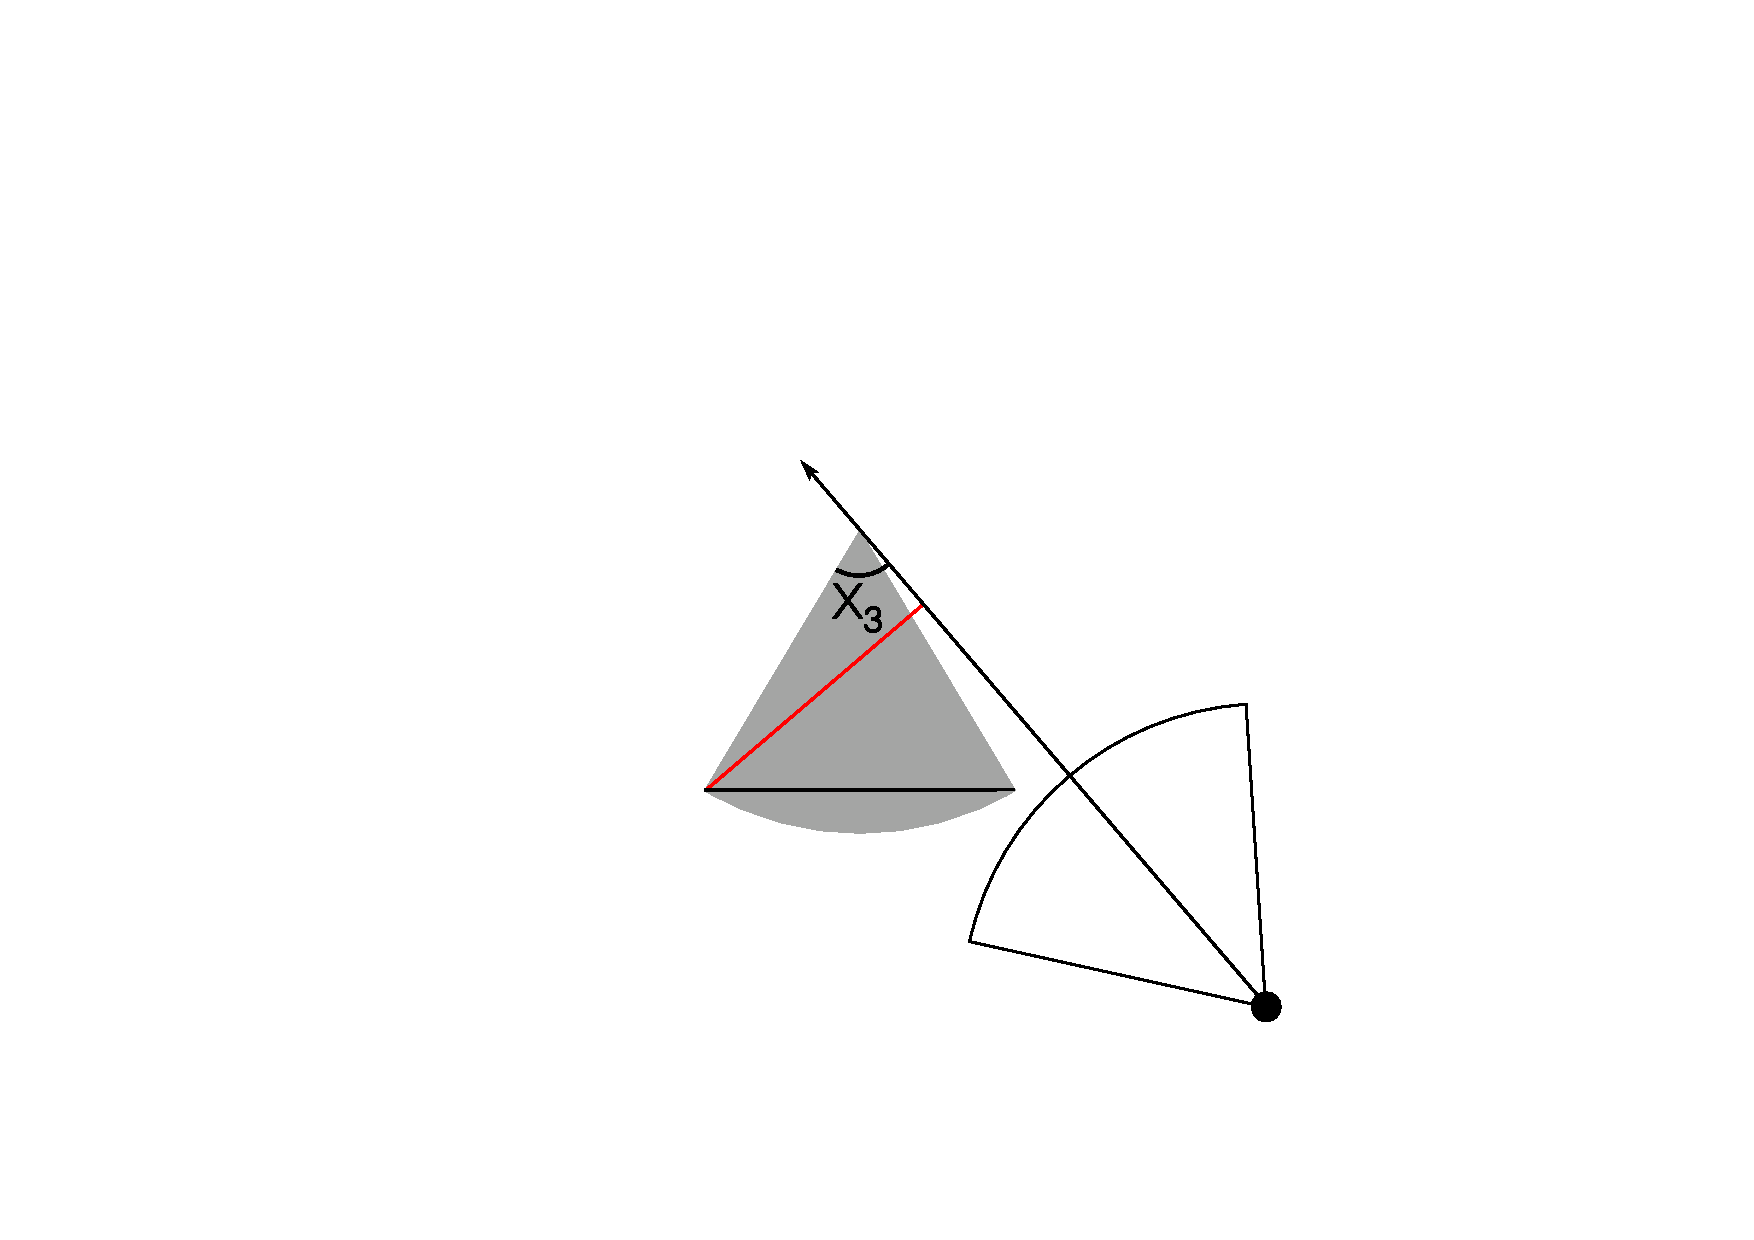
\includegraphics[width=.29\textwidth, trim=9cm 2cm 9cm 6cm]{imgs/x3.pdf}
  }
  \subfloat[$x_4$\label{fig:x4}]{
    \centering
    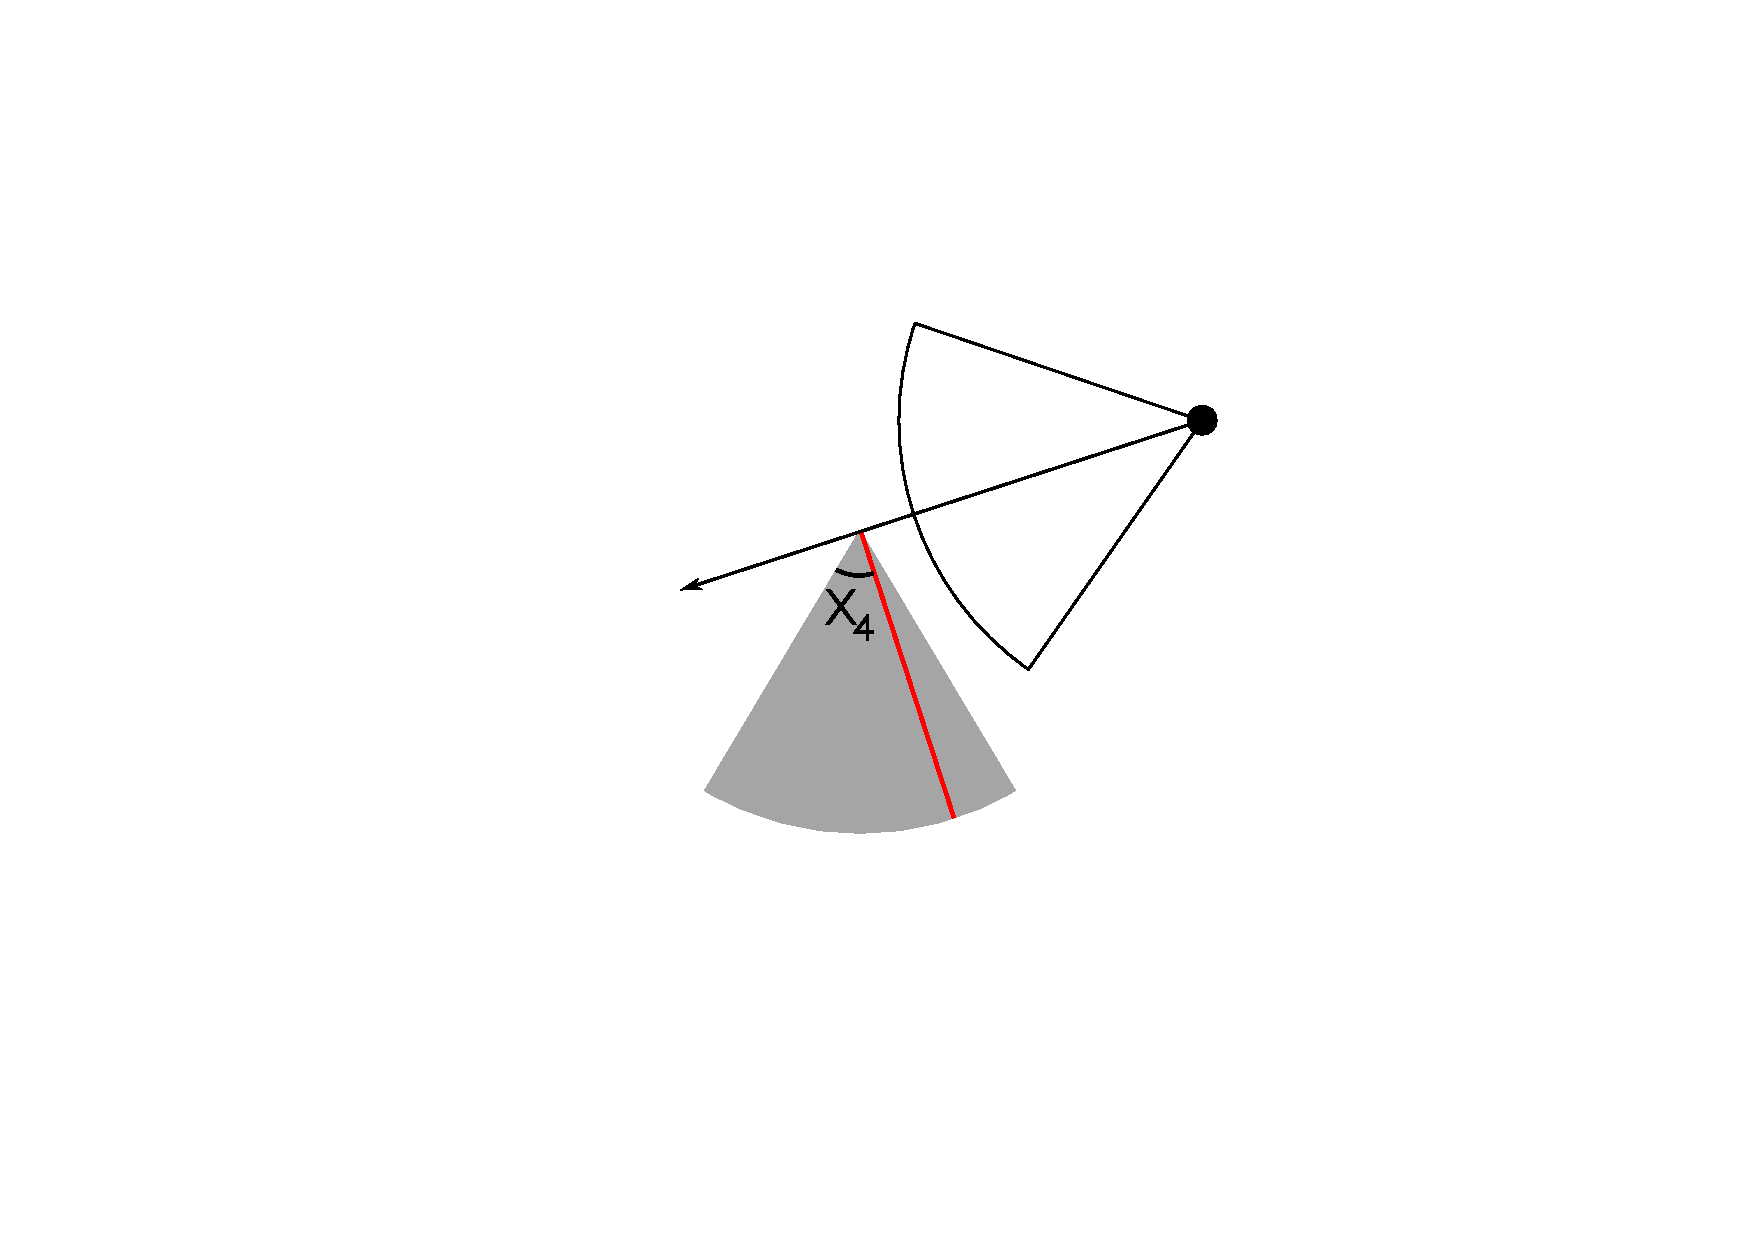
\includegraphics[width=.29\textwidth, trim=7cm 2cm 11cm 6cm]{imgs/x4.pdf}
  }
}
\caption[The location of the focal angles $x_{i\in[1,4]}$]{
The location of the focal angles $x_{i\in[1,4]}$.
$x_1$ is used in SE and NE models (including the gas model).
$x_2$ -- $x_4$ are used in NW and SW models.
The sector shaped detection region is shown in grey.
Animals are filled black circles and the animal signal is an unfilled sector.
The animals direction of movement is indicated with an arrow.
The profile $p$ is shown with a red line.
(a) Animal is directly approaching the sensor at $x_1$ = $\frac{\pi}{2}$.
(b) Animal is directly approaching the sensor at $x_2$ = $\frac{\pi}{2}$.
$x_2$ then decreases until the profile is perpendicular to the edge of the detection region.
(c) When the profile is perpendicular to the edge of the detection region, $x_3 = \theta$.
(d) $x_4$ measures the angle between the left side of the detection region and the profile.}

\label{fig:xis}
\end{figure}



In order to derive animal density, we need to consider relative velocity from the reference frame of the animals.
Conceptually, this requires us to imagine that all animals are stationary and randomly distributed in space, while the sensor moves with velocity $v$.
If we calculate the area covered by the sensor during the survey period we can estimate the number of animals the sensor should capture.
As a circle moving across a plane, the area covered by the sensor per unit time is $2rv$.
The number of expected captures, $z$, for a survey period of $t$, with an animal density of $D$ is $z = 2rvtD$.
To estimate the density, we rearrange to get $D = z/2rvt$.

\subsubsection{gREM derivations for different detection and signal widths}
Different combinations of $\theta$ and $\alpha$ would be expected to occur (\emph{e.g.}, sensors have different detection widths and animals have different signal widths).
For different combinations $\theta$ and $\alpha$, the area covered per unit time is no longer given by $2rv$.
Instead of the size of the sensor detection zone having a diameter of $2r$, the size changes with the approach angle between the sensor and the animal.
For any given signal width and detector width and depending on the angle that the animal approaches the sensor, the width of the area within which an animal can be detected is called the profile, $p$.
The size of the profile (averaged across all approach angles) is defined as the average profile $\bar{p}$.
However, different combinations of $\theta$ and $\alpha$ need different equations to calculate $\bar{p}$.
This $\bar{p}$ is the only thing that changes 

We have identified the parameter space for the combinations of $\theta$ and $\alpha$ for which the derivation of the equations are the same (defined as sub-models in the gREM) (Figure~\ref{fig:equalRegions}).
For example, the gas model becomes the simplest gREM sub-model (upper right in Figure~\ref{fig:equalRegions}) and the REM from \cite{rowcliffe2008estimating} is another gREM sub-model where $\theta<\pi/2$ and $\alpha = 2\pi$.

Models with $\theta = 2\pi$ are described first (the gas model described above and SE1).
Then models with $\theta > \pi$ are described (NE then SE).
Finally models with $\theta < \pi$ (NW then SW) are described.

\subsection{Model SE1} \label{SE1}
SE1 is very similar to the gas model except that because $\alpha \le \pi$ the profile width is no longer $2r$ but is instead limited by the width of the animal signal.
We therefore get a profile width of $2r\sin(\alpha/2)$ instead.

\begin{align}
    \bar{p}_{\text{\tiny{SE1}}} =&\frac{1}{\pi} \int\limits_{\frac{\pi}{2}}^{\frac{3 \pi}{2}}2 r \sin{\left (\frac{\alpha}{2} \right )}\;\mathrm{d}x_{1}\label{pSE1Def}\\
    \bar{p}_{\text{\tiny{SE1}}}  =& 2 r \sin{\left (\frac{\alpha}{2} \right )}\label{pSE1Sln}
\end{align}
This profile is integrated over the interval $[\frac{\pi}{2}, \frac{3\pi}{2}]$ which is $\pi$ radians of rotation starting with the animal moving directly towards the sensor (Figure~\ref{fig:xis}a).

\subsection{ Models NE1--3} \label{NE}

When the detection zone is not a circle, we have more complex profiles  and need to explicitly write functions for the width of the profile for every approach angle.
We then use these functions to find the average profile width $\bar{p}$ for all approach angles by integrating across all $2\pi$ angles of approach and dividing by $2\pi$.




\begin{figure}[t]
  \centering
{
  \subfloat[\label{fig:NELimit}]{
    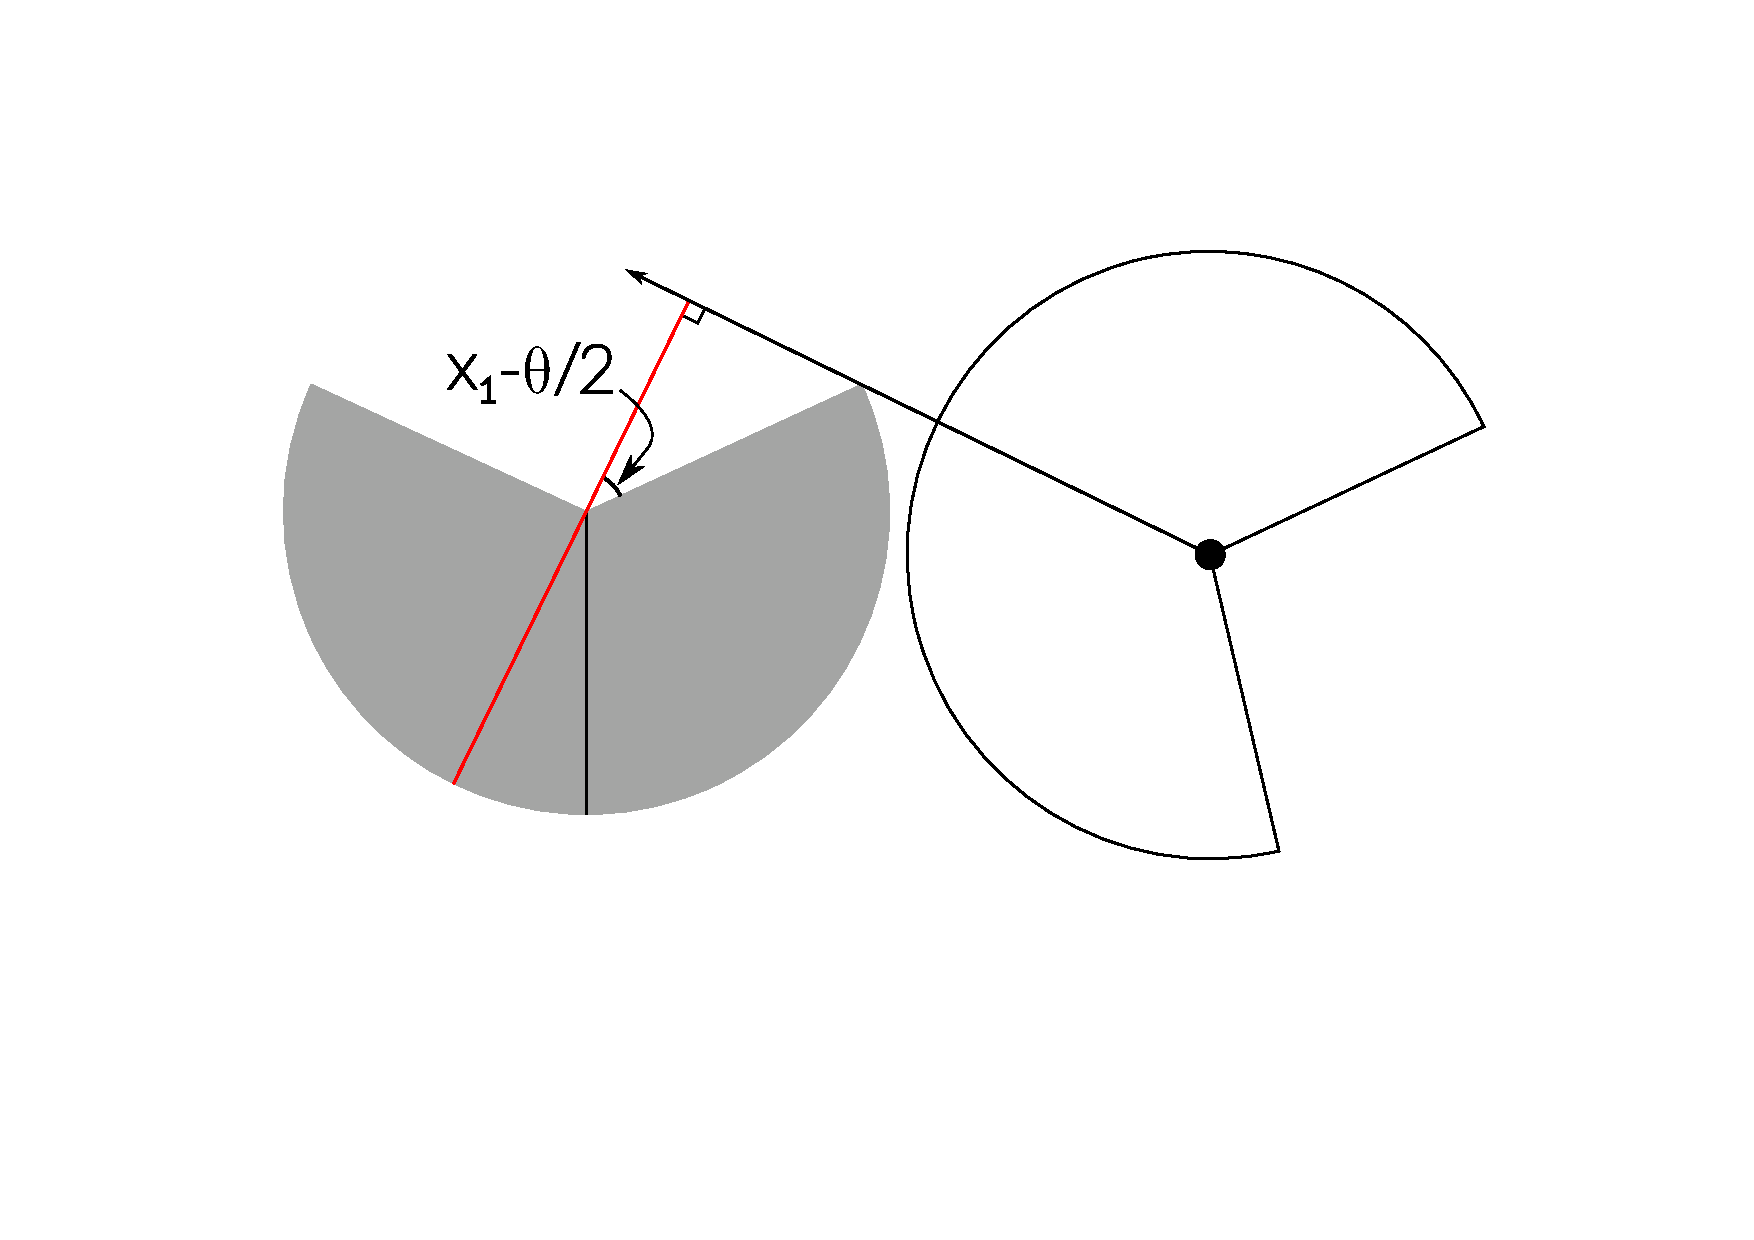
\includegraphics[width=.3\textwidth, trim=5cm 3cm 4cm 1cm]{imgs/ne2.pdf}
  } 
  \subfloat[\label{fig:NE3third}]{
    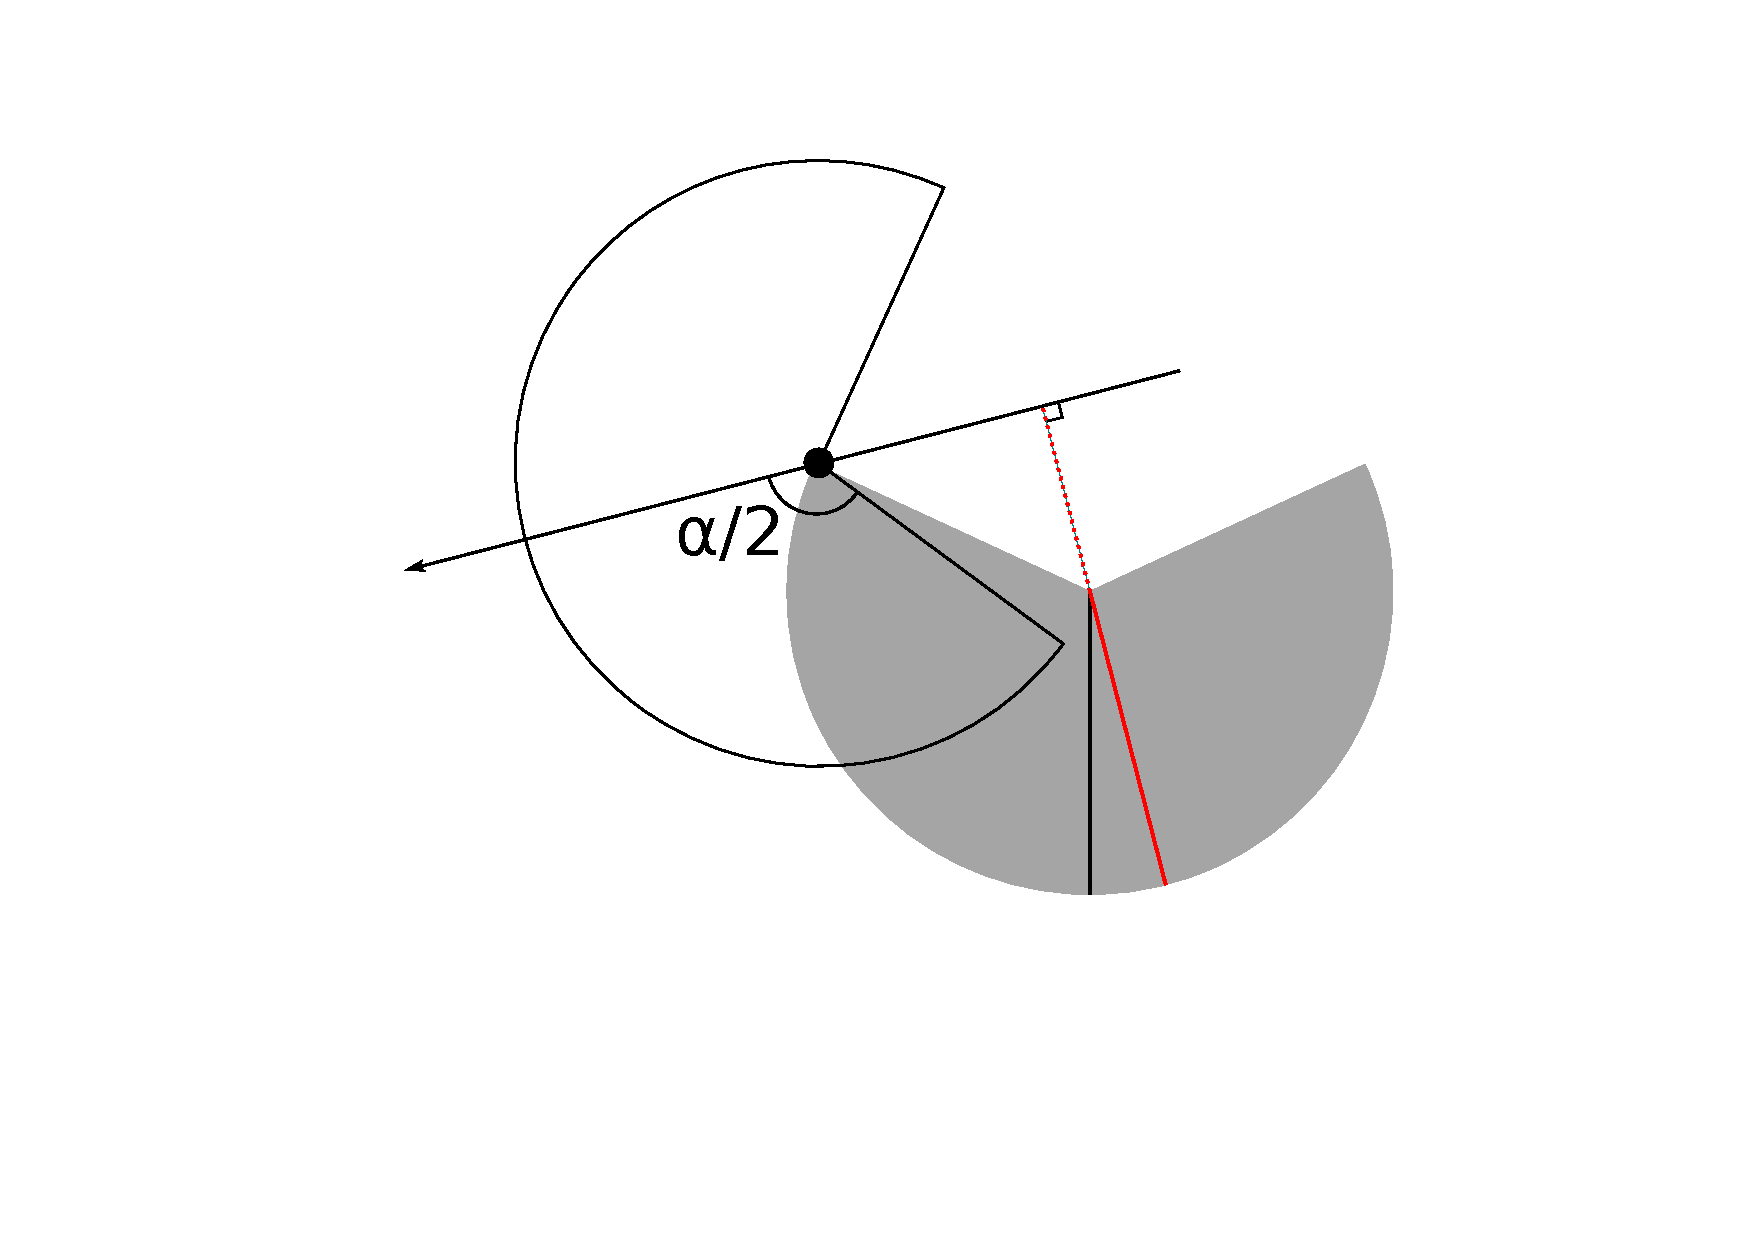
\includegraphics[width=.3\textwidth, trim=4cm 2cm 6cm 0cm]{imgs/ne33.pdf}
  }
  \subfloat[\label{fig:NE3fourth}]{
    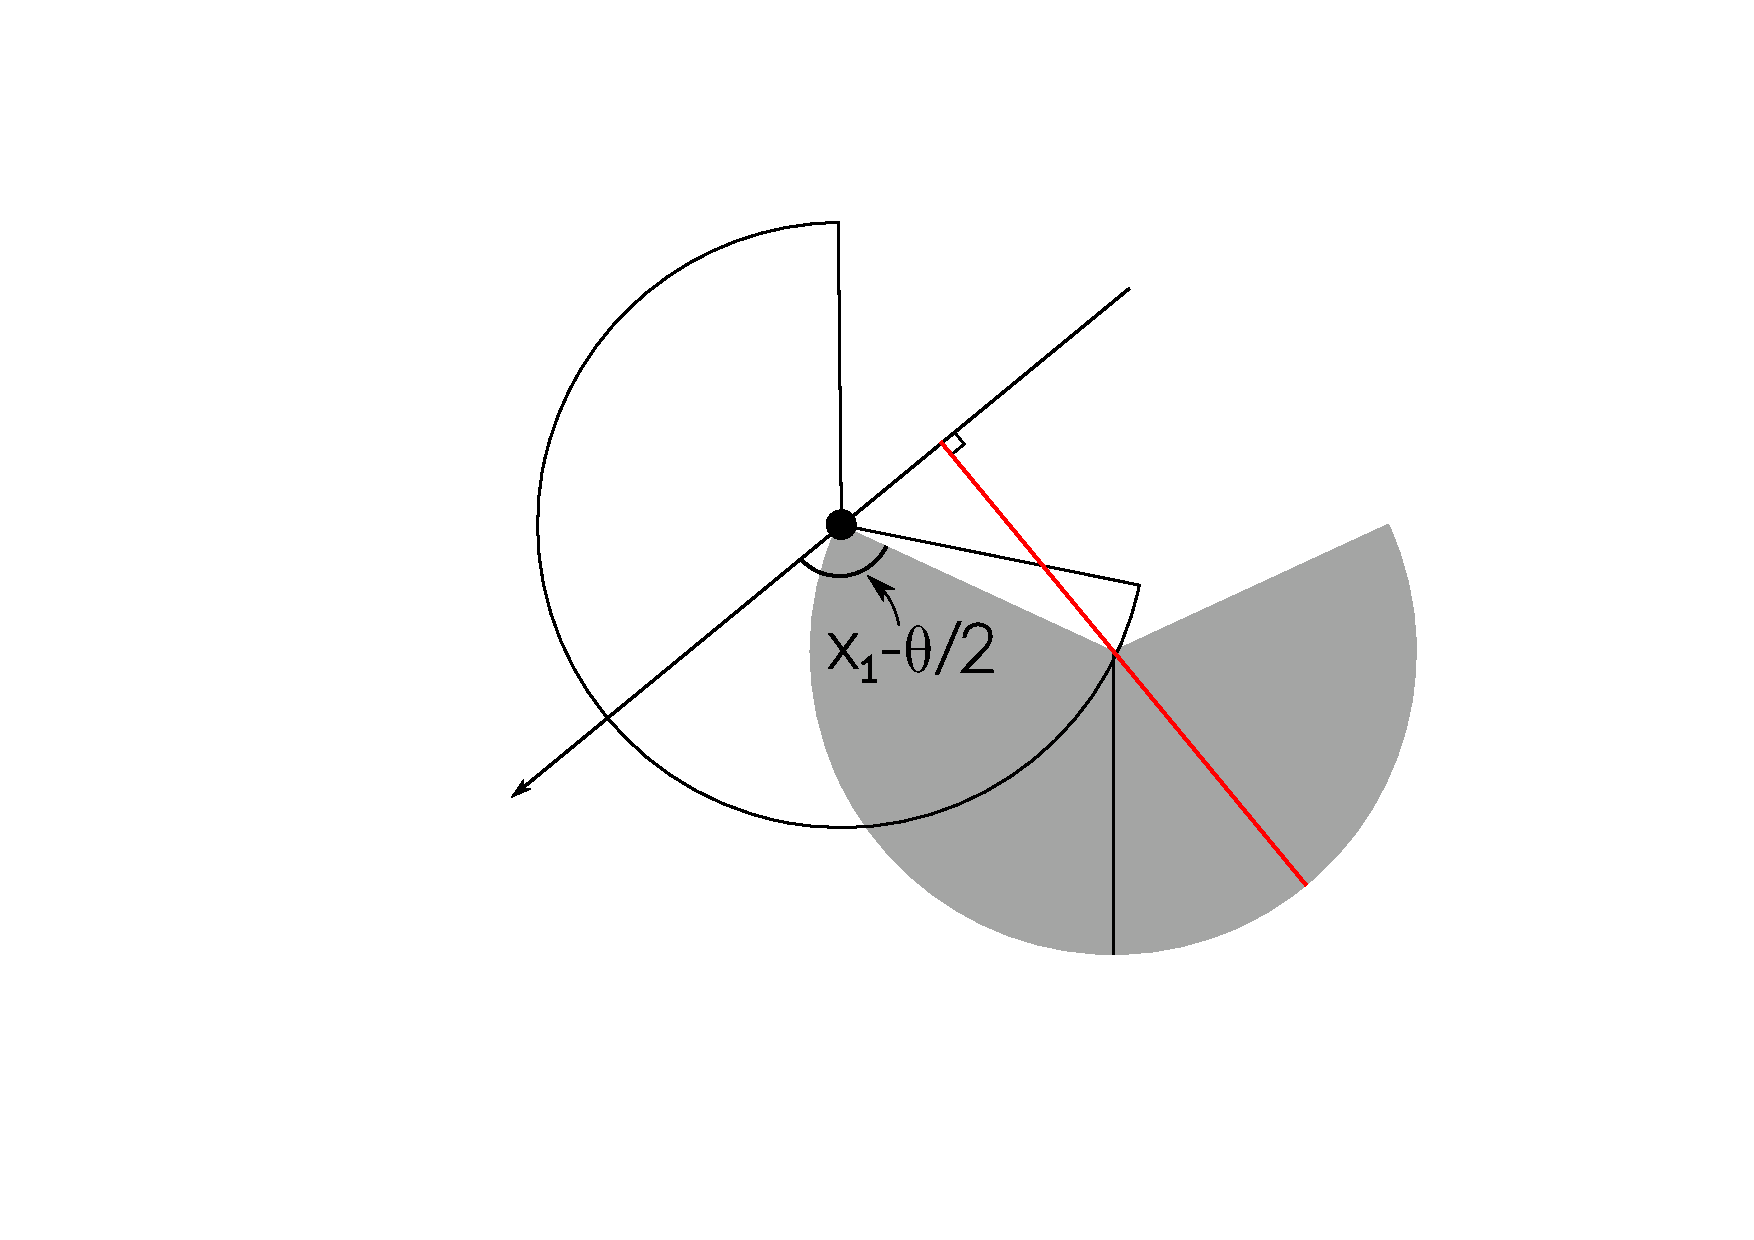
\includegraphics[width=.3\textwidth, trim=5cm 1cm 4cm 1cm]{imgs/ne34.pdf}
  }
}
\caption[Three of the integrals in NE models]{
Three of the integrals in NE models.
The sector shaped detection region is shown in grey.
Animals are filled black circles and the animal signal is an unfilled sector.
The animals direction of movement is indicated with an arrow.
The profile $p$ is shown with a red line.
Dashed red lines indicate areas where animals cannot be detected.
(a) The second integral in NE with width $r + r\cos(x_1 - \theta/2)$.
(b) The third integral in NE3.
$\alpha/2$ is labelled.
As it is small, animals to the right of the detector cannot be detected.
(c) After further rotation, $\alpha/2$ is now bigger than the angle shown and animals to the right of the detector can again be detected.
}
\label{fig:NE}
\end{figure}


\begin{figure}[t]
        \centering
        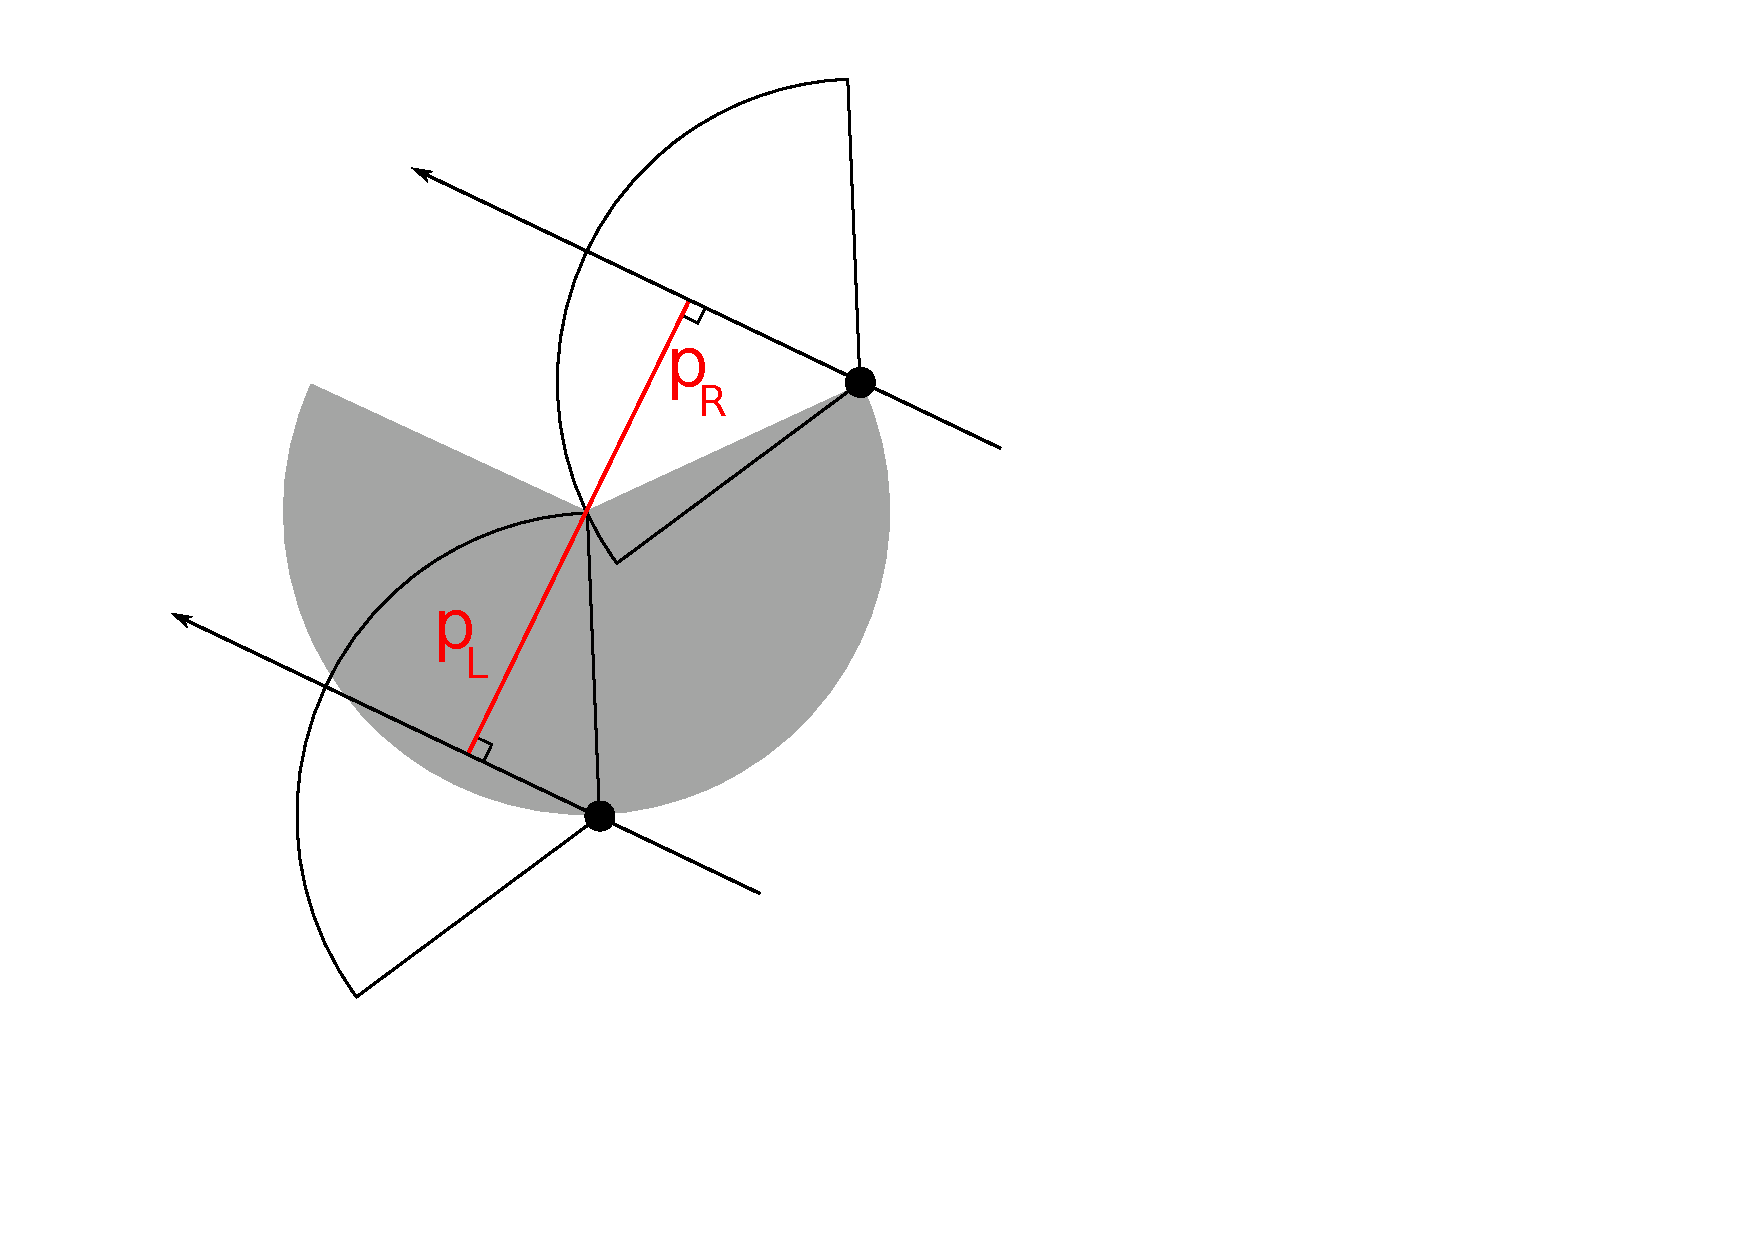
\includegraphics[width=0.35\textwidth, trim=1cm 4cm 9cm 1cm]{imgs/se3.pdf}
\caption[The second integral in SE]{The second integral in SE.
The right side of the profile ($p_R$) is limited by the size of the sensor region  while the left side of the profile ($p_L$) is limited by the size of the signal width.
The full profile has width $p = r\sin(\alpha/2) +r\cos(\theta/2-x_1)$.
The sector shaped detection region is shown in grey.
Animals are filled black circles and the animal signal is an unfilled sector.
The animals direction of movement is indicated with an arrow.
The profile $p$ is shown with a red line.
  }
\label{fig:se3}
\end{figure}

There are three submodels within quadrant NE (Figure~\ref{fig:equalRegions}).
Note that NE1 covers the area $\alpha=2\pi$ as well as the triangle below it as these two models are specified exactly the same, rather than happening to have equal results.

These models have up to five profiles.

\begin{enumerate}
\item The profile width starts, from $x_1=\frac{\pi}{2}$ as $2r$.
\item At $x_1 = \theta/2$, the right hand side of the profile cannot be $r$ wide as the corner of the `blind spot' limits its size to being $r\cos(x_1 - \theta/2)$ wide (Figure~\ref{fig:NELimit}).

\item The third profile is only found in NE3.
If $\alpha < 4\pi - 2\theta$, then at $x_1=\theta/2 + \pi/2$, when the profile is perpendicular to the edge of the blind spot, the whole right side of the profile is invisible to the sensor (Figure~\ref{fig:NE3third}).
This gives a profile size of just $r$.

\item At some point, the sensor can detect animals once they have passed the blind spot giving a profile width of $r + r\cos(x_1 + \theta/2)$ (Figure~\ref{fig:NE3fourth}).
From $x_1=\pi$, if the animal signal is wide enough to be detected in this area, this is the wider profile.
This then defines the split between NE1 and NE2.
In NE1, with $\alpha > 3\pi - \theta$, the animal signal is wide enough that at $x_1=\pi$ the animal can immediately be detected past the blind spot and so this profile is used.
In NE2, with $\alpha < 3\pi - \theta$, the latter profile is reached at $5\pi/2 - \theta/2 - \alpha/2$.

\item Finally, common to all three models, at $x_1 = 2\pi - \theta/2$ the profile becomes a full $2r$ once again.
\label{NElist5}
\end{enumerate}



\subsubsection{Model NE1} \label{NE1}

Submodel NE1 exists within the area bounded by $\alpha\le2\pi$, $\theta\le2\pi$ and $\alpha \ge 3\pi - \theta$ (Figure~\ref{fig:equalRegions}).
It has four profiles; it does not include the $r$ profile at $x_1=\pi$ (profile described in point (3) in Section \ref{NE}).
Furthermore, $\theta$ is wide enough that the $r + r\cos(x_1 + \theta/2)$ profile starts at $\pi$.
This then gives us


\begin{align}
    \bar{p}_{\text{\tiny{NE1}}} =&\frac{1}{\pi} \left(\;\;\int\limits_{\frac{\pi}{2}}^{\frac{\theta}{2}}2 r\;\mathrm{d}x_{1}+\int\limits_{\frac{\theta}{2}}^{\pi}r \cos{\left (\frac{\theta}{2} - x_{1} \right )} + r\;\mathrm{d}x_{1}\right.\notag\\
 &\left.+\int\limits_{\pi}^{2 \pi - \frac{\theta}{2}}r \cos{\left (\frac{\theta}{2} + x_{1} \right )} + r\;\mathrm{d}x_{1}+\int\limits_{2 \pi - \frac{\theta}{2}}^{\frac{3 \pi}{2}}2 r\;\mathrm{d}x_{1}\right)\label{pNE1Def}\\
    \bar{p}_{\text{\tiny{NE1}}}  =& \frac{r}{\pi} \left(\theta + 2 \sin{\left (\frac{\theta}{2} \right )}\right)\label{pNE1Sln}
\end{align}





\subsubsection{Model NE2} \label{NE2}

Model NE2 is bounded by $\alpha \le 3\pi - \theta$, $\alpha \ge 4\pi - 2\theta$ and $\alpha \ge \pi$ (Figure~\ref{fig:equalRegions}).
It is the same as NE1 except that the third profile starts at $5\pi/2 - \theta/2 - \alpha/2$ instead of at $\pi$ which is reflected in the different bounds in the second and third integral.

\begin{align}
    \bar{p}_{\text{\tiny{NE2}}} =&\frac{1}{\pi} \left(\;\;\int\limits_{\frac{\pi}{2}}^{\frac{\theta}{2}}2 r\;\mathrm{d}x_{1}+\int\limits_{\frac{\theta}{2}}^{\frac{5 \pi}{2} - \frac{\theta}{2} - \frac{\alpha}{2}}r \cos{\left (\frac{\theta}{2} - x_{1} \right )} + r\;\mathrm{d}x_{1}\right.\notag\\
 &\left.+\int\limits_{\frac{5 \pi}{2} - \frac{\theta}{2} - \frac{\alpha}{2}}^{2 \pi - \frac{\theta}{2}}r \cos{\left (\frac{\theta}{2} + x_{1} \right )} + r\;\mathrm{d}x_{1}+\int\limits_{2 \pi - \frac{\theta}{2}}^{\frac{3 \pi}{2}}2 r\;\mathrm{d}x_{1}\right)\label{pNE2Def}\\
    \bar{p}_{\text{\tiny{NE2}}}  =& \frac{r}{\pi} \left(\theta - \cos{\left (\frac{\alpha}{2} \right )} + \cos{\left (\frac{\alpha}{2} + \theta \right )}\right)\label{pNE2Sln}
\end{align}

\subsubsection{Model NE3} \label{NE3}

Model NE3 is bound by $\alpha \le 4\pi - 2\theta$, $\alpha \ge \pi$ and $\theta \ge \pi$ (Figure~\ref{fig:equalRegions}).
It is the same as NE2 except that it contains the extra profile with width $r$ (third integral).

\begin{align}
    \bar{p}_{\text{\tiny{NE3}}} =&\frac{1}{\pi} \left(\;\;\int\limits_{\frac{\pi}{2}}^{\frac{\theta}{2}}2 r\;\mathrm{d}x_{1}+\int\limits_{\frac{\theta}{2}}^{\frac{\theta}{2} + \frac{\pi}{2}}r \cos{\left (\frac{\theta}{2} - x_{1} \right )} + r\;\mathrm{d}x_{1}\right.\notag\\
 &\left.+\int\limits_{\frac{\theta}{2} + \frac{\pi}{2}}^{\frac{5 \pi}{2} - \frac{\theta}{2} - \frac{\alpha}{2}}r\;\mathrm{d}x_{1}+\int\limits_{\frac{5 \pi}{2} - \frac{\theta}{2} - \frac{\alpha}{2}}^{2 \pi - \frac{\theta}{2}}r \cos{\left (\frac{\theta}{2} + x_{1} \right )} + r\;\mathrm{d}x_{1}+\int\limits_{2 \pi - \frac{\theta}{2}}^{\frac{3 \pi}{2}}2 r\;\mathrm{d}x_{1}\right)\label{pNE3Def}\\
    \bar{p}_{\text{\tiny{NE3}}}  =& \frac{r}{\pi} \left(\theta - \cos{\left (\frac{\alpha}{2} \right )} + 1\right)\label{pNE3Sln}
\end{align}




\subsection{Models SE2--4} \label{SE}

Quadrant SE contains three submodels excluding SE1  (Figure~\ref{fig:equalRegions}).
The differences between these three models are similar to the differences between the models in NE.
There are four possible profiles.
\begin{enumerate}
\item As $\alpha$ is less than $\pi$ the profile is smaller than $2r$, even when the sensor width is a full diameter.
The profile width starts as $2r\sin(\alpha/2)$.
\item Similar to NE, at a certain point the blind spot of the sensor area limits the profile width on one side.
This gives a profile width of $r\sin(\alpha/2) + r\cos(x_1 - \theta/2)$ (Figure~\ref{fig:se3}).
\item Also similar to NE, there can be a point where the right side of the profile is 0 giving a profile width of $r\sin(\alpha/2)$.
\item If $\alpha \le 2\pi - \theta$, then at $x_1 = \theta/2 + \pi/2 + \alpha/2 $ the profile width becomes 0.
This inequality distinguishes between SE3 and SE4.
\item The third profile $r\sin(\alpha/2)$ starts at $\theta/2 + \pi/2$ while at $5\pi/2 - \alpha/2 - \theta/2$ the profile returns to size $2r\sin(\alpha/2)$.
If $\theta/2 + \pi/2 \ge 5\pi/2 - \alpha/2 - \theta/2$ we go straight into the  $2r\sin(\alpha/2)$ profile and miss the $r\sin(\alpha/2)$ profile.
 SE2 and SE3 are separated by this inequality which simplifies to $\alpha \le 4\pi - 2\theta$.

\end{enumerate}





\subsubsection{Model SE2} \label{SE2}

SE2 is bounded by $\alpha \ge 4\pi - 2\theta$, $\alpha \le \pi$ and $\theta \le 2\pi$ (Figure~\ref{fig:equalRegions}).
As $\alpha \ge 4\pi - 2\theta$, there is no $r\sin(\alpha/2)$ profile.
As $\alpha \le 4\pi - 2\theta$, the profile returns to $2r\sin(\alpha/2)$ rather than going to 0.
These integrals relate to profiles (1), (2) and (5) in Section \ref{SE}.

\begin{align}
    \bar{p}_{\text{\tiny{SE2}}} =&\frac{1}{\pi} \left(\;\;\int\limits_{\frac{\pi}{2}}^{\frac{\pi}{2} + \frac{\theta}{2} - \frac{\alpha}{2}}2 r \sin{\left (\frac{\alpha}{2} \right )}\;\mathrm{d}x_{1}+\int\limits_{\frac{\pi}{2} + \frac{\theta}{2} - \frac{\alpha}{2}}^{\frac{5 \pi}{2} - \frac{\theta}{2} - \frac{\alpha}{2}}r \sin{\left (\frac{\alpha}{2} \right )} + r \cos{\left (\frac{\theta}{2} - x_{1} \right )}\;\mathrm{d}x_{1}\right.\notag\\
 &+\left.\int\limits_{\frac{5 \pi}{2} - \frac{\theta}{2} - \frac{\alpha}{2}}^{\frac{3 \pi}{2}}2 r \sin{\left (\frac{\alpha}{2} \right )}\;\mathrm{d}x_{1}\right)\label{pSE2Def}\\
    \bar{p}_{\text{\tiny{SE2}}}  =& \frac{r}{\pi} \left(\theta \sin{\left (\frac{\alpha}{2} \right )} - \cos{\left (\frac{\alpha}{2} \right )} + \cos{\left (\frac{\alpha}{2} + \theta \right )}\right)\label{pSE2Sln}
\end{align}



\subsubsection{Model SE3} \label{SE3}

SE3 is bounded by $4\pi - 2\theta \le \alpha \le 4\pi - 2\theta$ and $\alpha \le \pi$ (Figure~\ref{fig:equalRegions}).
Therefore there is a $r\sin(\alpha/2)$ profile but no $0r$ profile.
This relates to profiles (1), (2), (3) and (5) above.

\begin{align}
    \bar{p}_{\text{\tiny{SE3}}} =&\frac{1}{\pi} \left(\;\;\int\limits_{\frac{\pi}{2}}^{\frac{\pi}{2} + \frac{\theta}{2} - \frac{\alpha}{2}}2 r \sin{\left (\frac{\alpha}{2} \right )}\;\mathrm{d}x_{1}+\int\limits_{\frac{\pi}{2} + \frac{\theta}{2} - \frac{\alpha}{2}}^{\frac{\theta}{2} + \frac{\pi}{2}}r \sin{\left (\frac{\alpha}{2} \right )} + r \cos{\left (\frac{\theta}{2} - x_{1} \right )}\;\mathrm{d}x_{1}\right.\notag\\
 &\left.+\int\limits_{\frac{\theta}{2} + \frac{\pi}{2}}^{\frac{5 \pi}{2} - \frac{\theta}{2} - \frac{\alpha}{2}}r \sin{\left (\frac{\alpha}{2} \right )}\;\mathrm{d}x_{1}+\int\limits_{\frac{5 \pi}{2} - \frac{\theta}{2} - \frac{\alpha}{2}}^{\frac{3 \pi}{2}}2 r \sin{\left (\frac{\alpha}{2} \right )}\;\mathrm{d}x_{1}\right)\label{pSE3Def}\\
    \bar{p}_{\text{\tiny{SE3}}}  =& \frac{r}{\pi} \left(\theta \sin{\left (\frac{\alpha}{2} \right )} - \cos{\left (\frac{\alpha}{2} \right )} + 1\right)\label{pSE3Sln}
\end{align}

\subsubsection{Model SE4} \label{SE4}

Finally SE4 is bounded by  $\alpha \le 4\pi - 2\theta $, $\alpha\le\pi$ and $\theta \le \pi$ (Figure~\ref{fig:equalRegions}).
It is the same as SE3 except that the profile becomes 0 rather than returning to $2r\sin(\alpha/2)$.
This relates to profiles (1), (2), (3) and (4) above though profile (4) with width 0 is not shown.

\begin{align}
    \bar{p}_{\text{\tiny{SE4}}} =&\frac{1}{\pi} \left(\;\;\int\limits_{\frac{\pi}{2}}^{\frac{\pi}{2} + \frac{\theta}{2} - \frac{\alpha}{2}}2 r \sin{\left (\frac{\alpha}{2} \right )}\;\mathrm{d}x_{1}+\int\limits_{\frac{\pi}{2} + \frac{\theta}{2} - \frac{\alpha}{2}}^{\frac{\theta}{2} + \frac{\pi}{2}}r \sin{\left (\frac{\alpha}{2} \right )} + r \cos{\left (\frac{\theta}{2} - x_{1} \right )}\;\mathrm{d}x_{1}\right.\notag\\
 &\left.+\int\limits_{\frac{\theta}{2} + \frac{\pi}{2}}^{\frac{\alpha}{2} + \frac{\theta}{2} + \frac{\pi}{2}}r \sin{\left (\frac{\alpha}{2} \right )}\;\mathrm{d}x_{1}\right)\label{pSE4Def}\\
    \bar{p}_{\text{\tiny{SE4}}}  =& \frac{r}{\pi} \left(\theta \sin{\left (\frac{\alpha}{2} \right )} - \cos{\left (\frac{\alpha}{2} \right )} + 1\right)\label{pSE4Sln}
\end{align}



\begin{figure}[t]
  \centering
{
  \subfloat[\label{fig:NW1AT}]{
    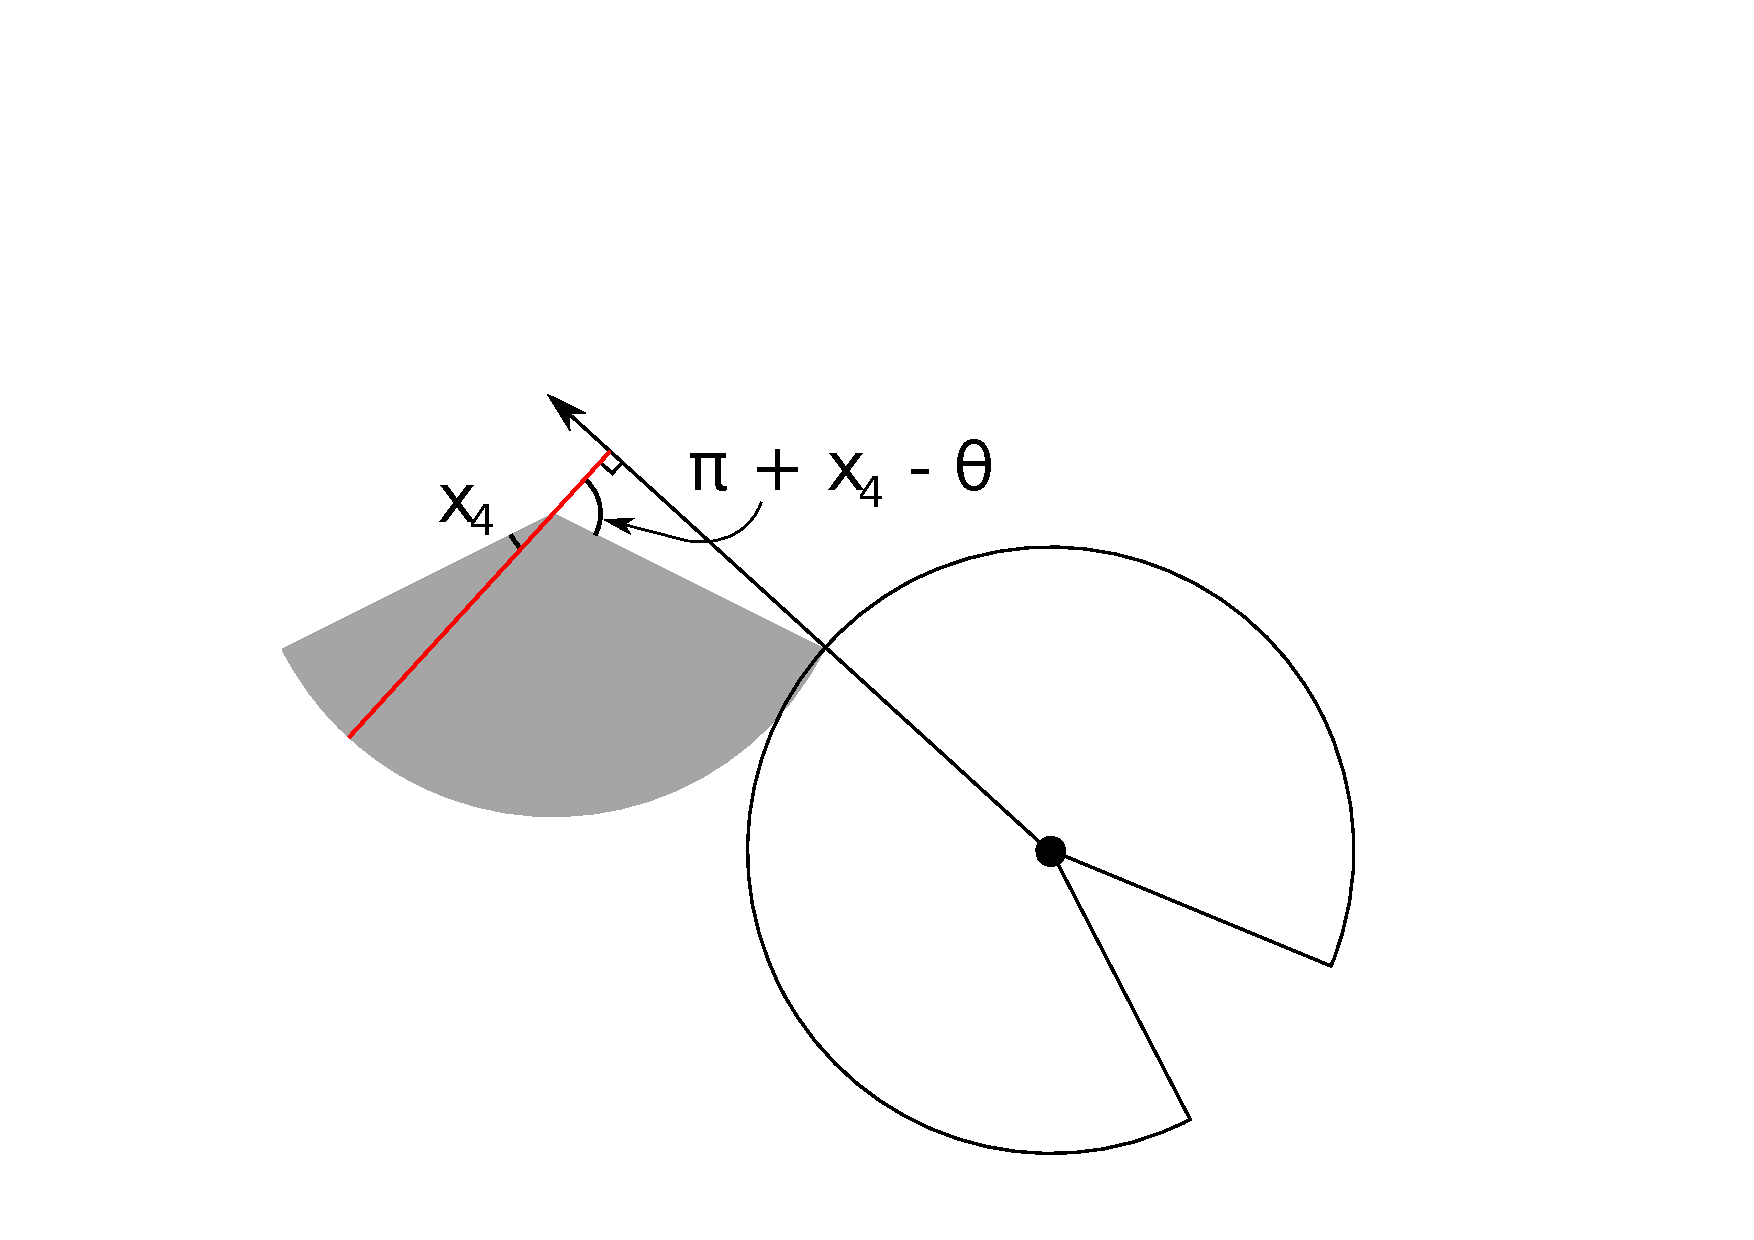
\includegraphics[width=0.5\textwidth, trim=5cm 1cm 4cm 1cm]{imgs/nw2.pdf}
  }
  \subfloat[\label{fig:NW1behindFull}]{
    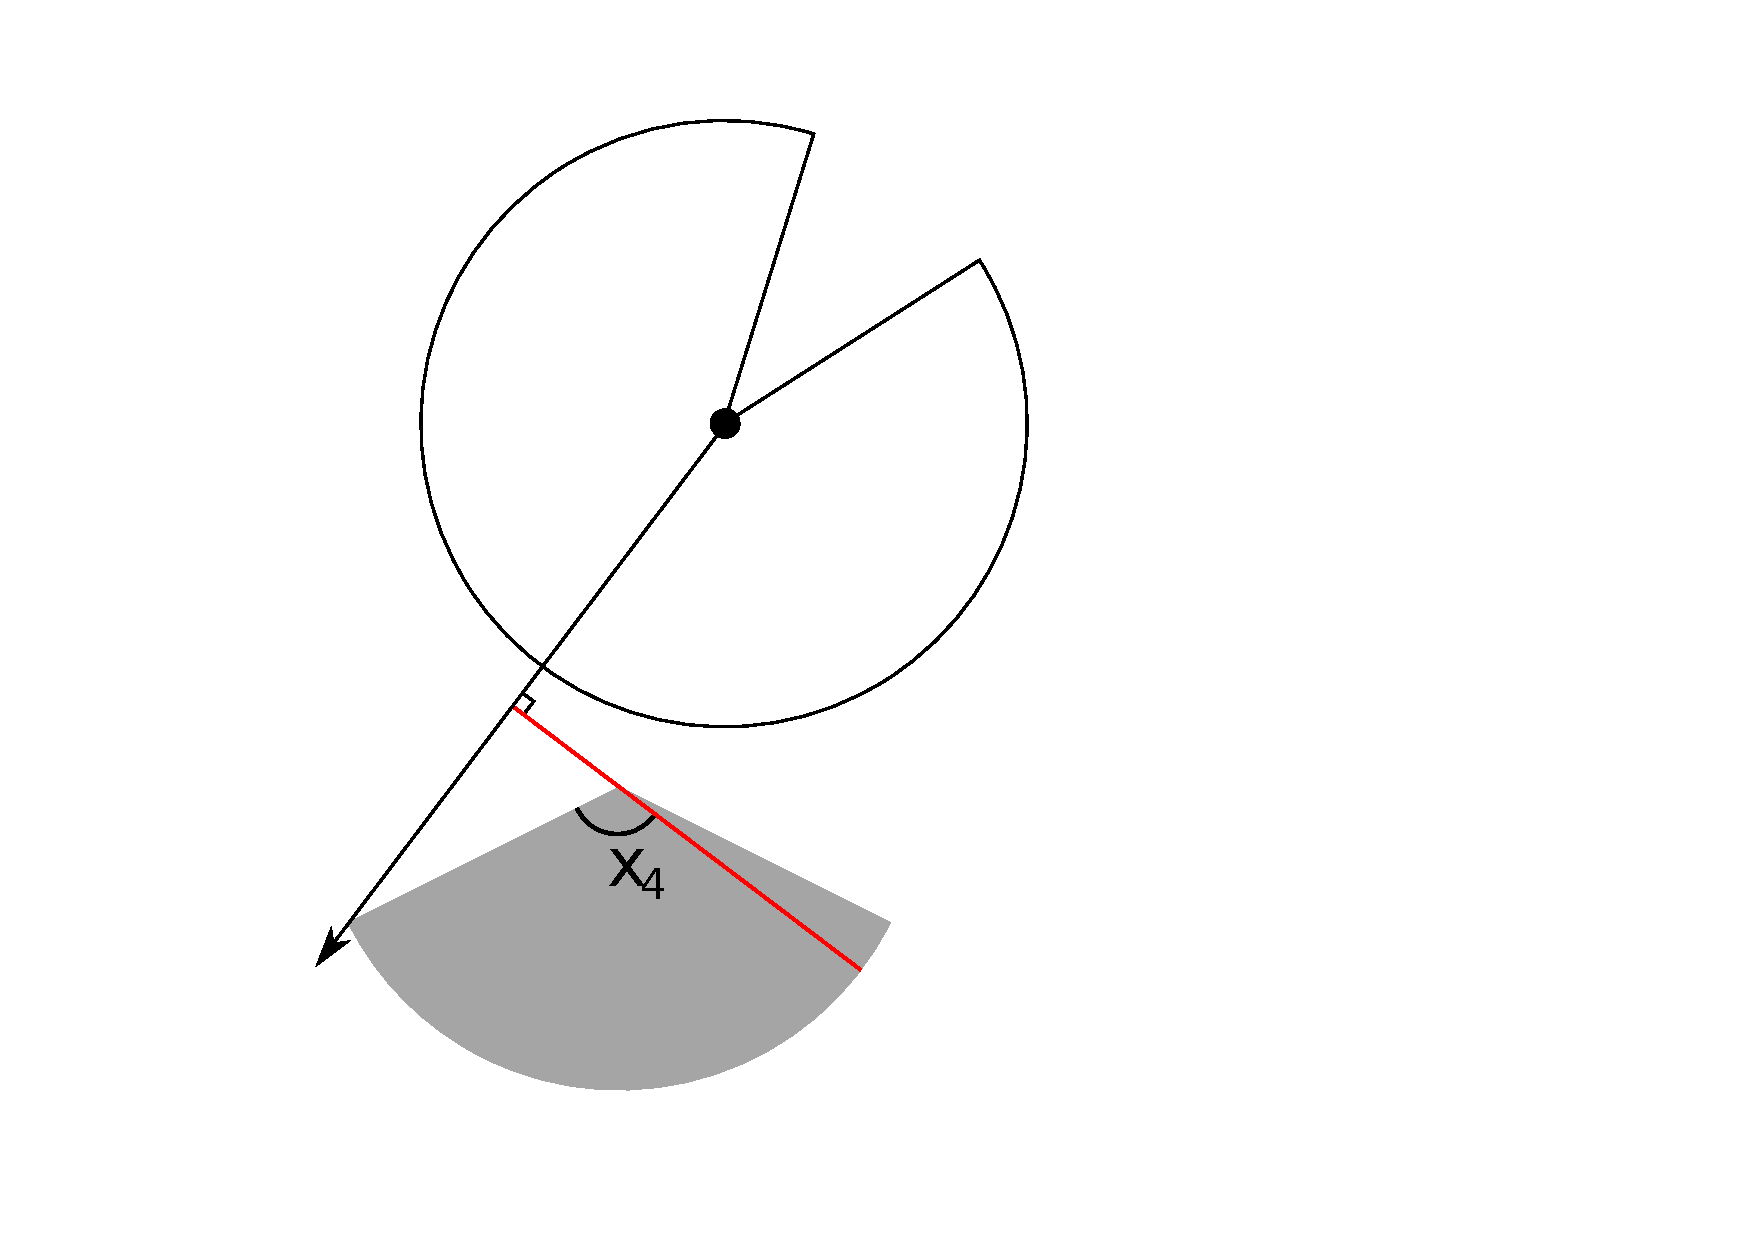
\includegraphics[width=0.5\textwidth, trim=0cm 1cm 4cm 1cm]{imgs/nw4.pdf}
  }
}
\caption[The second and fourth profiles of NW1]{
The second and fourth profiles of NW1.
The left side of of both profiles is of width $r$ while the right side differs.
(a) The right side of the profile is $r\cos(\pi+x_4-\theta) = - r\cos(\theta - x_4 )$ 
(b) The right side is $r\cos(\pi-x_4) = - r\cos x_4$ respectively.
In both images the sector shaped detection region is shown in grey.
Animals are filled black circles and the animal signal is an unfilled sector.
The animals direction of movement is indicated with an arrow.
The profile $p$ is shown with a red line.
}
\label{fig:NW1}
\end{figure}

\subsection{Model NW1} \label{NW1}

NW1 is the first model with $\theta < \pi$.
Whereas previously the focal angle has always been $x_1$, we now use different focal angles.
$x_2$ and $x_3$ correspond to $\gamma_1$ and $\gamma_2$ in \cite{rowcliffe2008estimating} while $x_4$ is new.
They are described in Figure~\ref{fig:xis}b--d.

There are five different profiles in NW1.
\begin{enumerate}
\item $x_2$ has an interval of $[\pi/2, \theta/2]$ which is from the angle of approach being directly towards the sensor until the profile is parallel to the left hand radius of the sensor sector (Figure~\ref{fig:x2}).
During this interval the profile width is $2r\sin\left(\theta/2\right)\sin(x_2)$ which is calculated using the equation for the length of a chord .
Note that while rotating anti-clockwise (as usual) $x_2$ decreases in size.
\item From here, we examine focal angle $x_4$ (note that $x_3$ is used in later models, but is not relevant here).  The left side of the profile is a full radius while the right side is limited to $- r\cos(x_4 - \theta)$ (Figure~\ref{fig:NW1AT}).
\item At $x_4 =  \theta - \pi/2$, the profile is perpendicular to the edge of the sensor area.
Here, the right side of the profile is $0r$ giving a profile size of $r$.
  %@tim is left side r?
\item When $x_4 = \pi/2$ the angle of approach is from behind the sensor, but we can once again be detected on the right side of the sensor (Figure~\ref{fig:NW1behindFull}).
Therefore the width of the profile is $r - r\cos(x_4)$.
\item  Finally, we have the $x_2$ profile, but from behind.
\end{enumerate}



\begin{align}
    \bar{p}_{\text{\tiny{NW1}}} =&\frac{1}{\pi} \left(\;\;\int\limits_{\frac{\theta}{2}}^{\frac{\pi}{2}}2 r \sin{\left (\frac{\theta}{2} \right )} \sin{\left (x_{2} \right )}\;\mathrm{d}x_{2}+\int\limits_{0}^{\theta - \frac{\pi}{2}}r - r \cos{\left (- x_{4} + \theta \right )}\;\mathrm{d}x_{4}\right.\notag\\
 &\left.+\int\limits_{\theta - \frac{\pi}{2}}^{\frac{\pi}{2}}r\;\mathrm{d}x_{4}+\int\limits_{\frac{\pi}{2}}^{\theta}r - r \cos{\left (x_{4} \right )}\;\mathrm{d}x_{4}+\int\limits_{\frac{\theta}{2}}^{\frac{\pi}{2}}2 r \sin{\left (\frac{\theta}{2} \right )} \sin{\left (x_{2} \right )}\;\mathrm{d}x_{2}\right)\label{pNW1Def}\\
    \bar{p}_{\text{\tiny{NW1}}}  =& \frac{r}{\pi} \left(\theta + 2\right)\label{pNW1Sln}
\end{align}

\subsection{Models NW2--4} \label{NW2--4}
% @tim this is still crap
The models NW2--4 have the five potential profiles in NW1 but not all profiles occur in each model, and the angle at which transitions occur are different.
Furthermore, there is one extra profile possible.
\begin{enumerate}
\item When approaching the sensor from behind, there is a period where the profile is $r$ wide as in NW1 profile (3).
\item At some point after profile (1) animals to the right of the sensor can be detected again.
If this occurs in the $x_4$ region, the profile width becomes  $r - r\cos(x_4)$ as in NW1.
\item However, as $\alpha$ is now less than $2\pi$, animals to the right of the sensor may be undetectable until we are in the second $x_2$ region.
In this case, when we first enter the second $x_2$ region, the profile has a width of $r\cos(x_2 - \theta/2)$.
This occurs only if $\alpha \le 3\pi - 2\theta$.
This inequality is found by noting that animals to the right of the sensor can be detected again at $x_4 = 3\pi/2 - \alpha$ but the $x_2$ region starts at $x_4 = \theta$.
The new profile in $x_2$ will only occur if  $ \theta < 3\pi/2 - \alpha/2$ which is rearranged to find the inequality above.
This defines the boundary between NW2 and NW3.
\item As $\alpha \le 2\pi$ it is possible that when the angle of approach is from directly behind the sensor the animal will not be detected at all.
This is the case if $\alpha/2\le \pi-\theta/2$ (Figure~\ref{fig:NW2--4}).
This inequality (simplified as $\alpha\le 2\pi-\theta$) defines the boundary between NW3 and NW4.
\end{enumerate}



\begin{figure}[t]
  \centering
{
  \subfloat[\label{fig:NW2--4behind}]{
    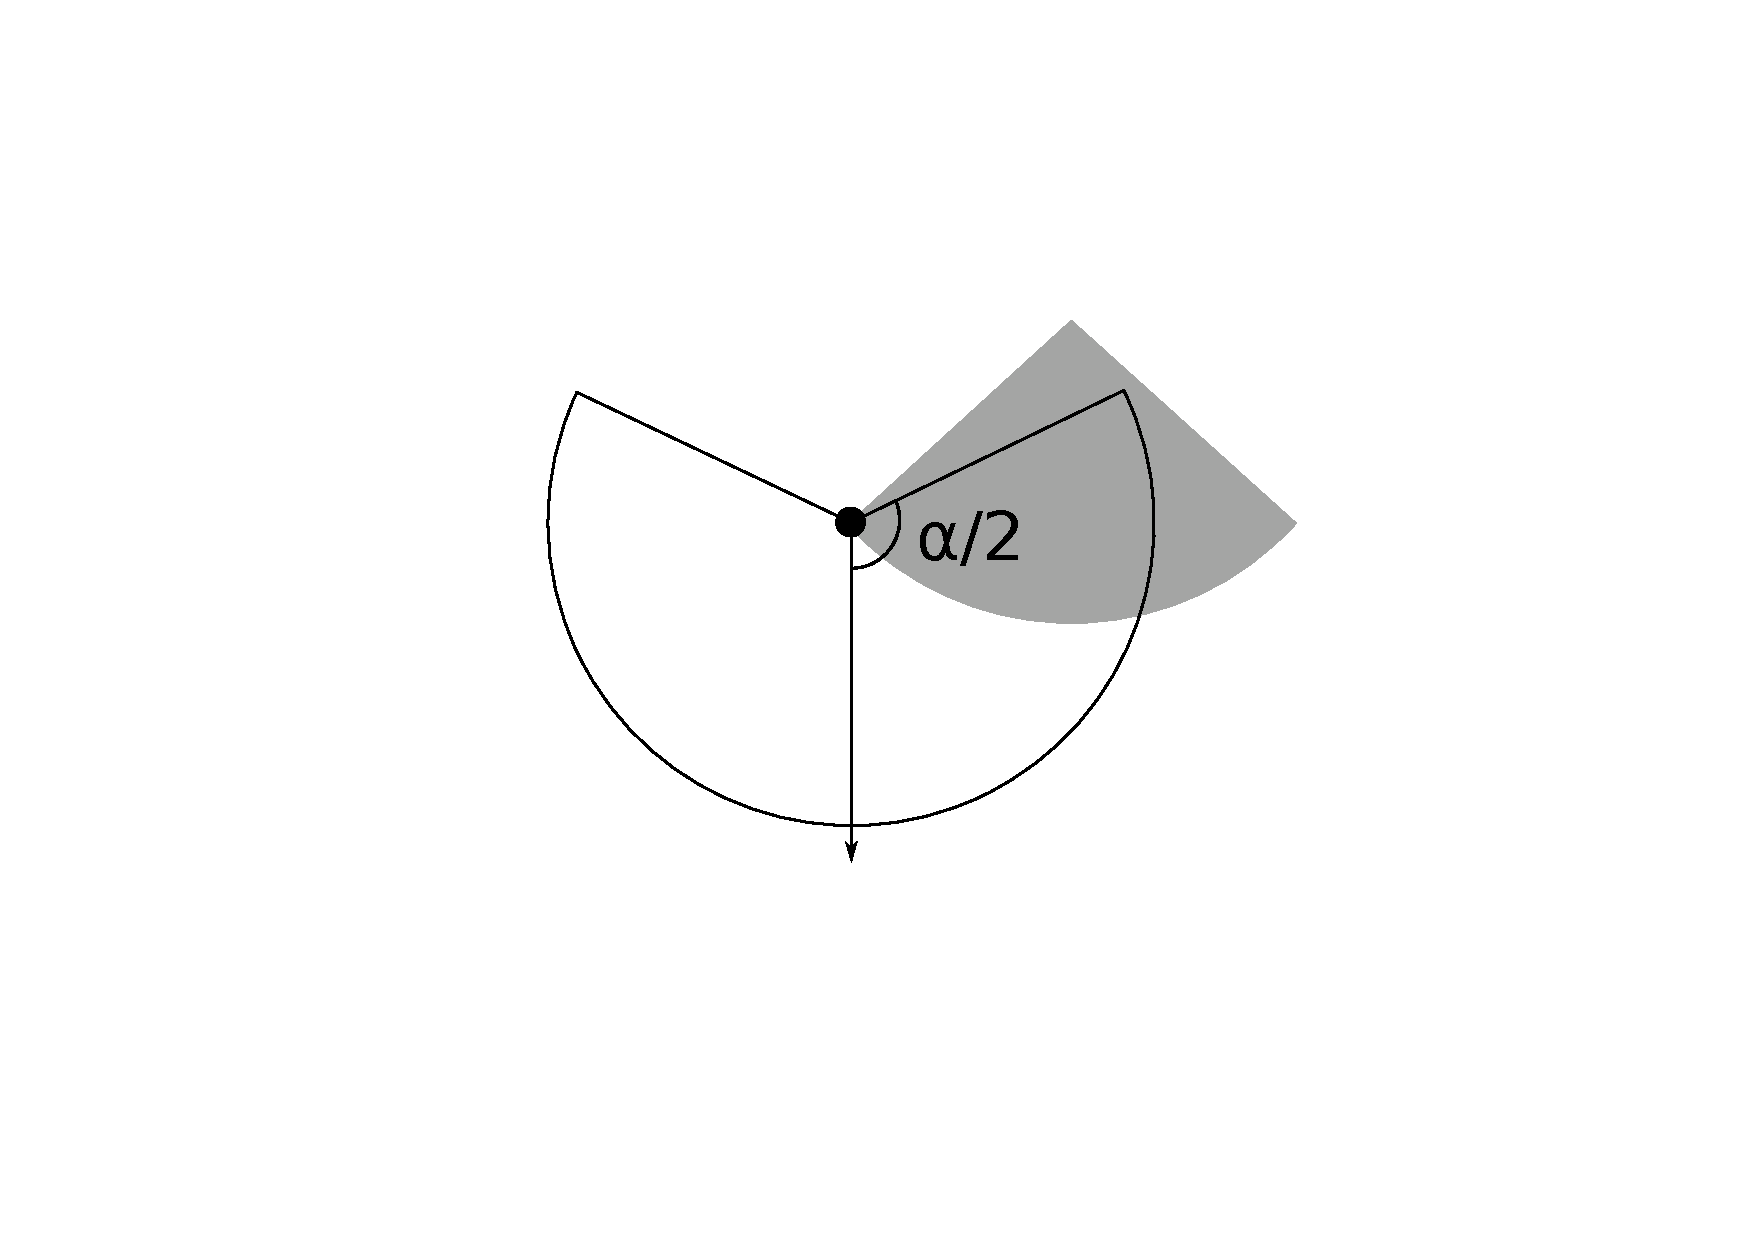
\includegraphics[width=0.45\textwidth, trim=5cm 6cm 4cm 1cm]{imgs/behind.pdf}   
  }
  \subfloat[\label{fig:NW2--4behind2}]{
    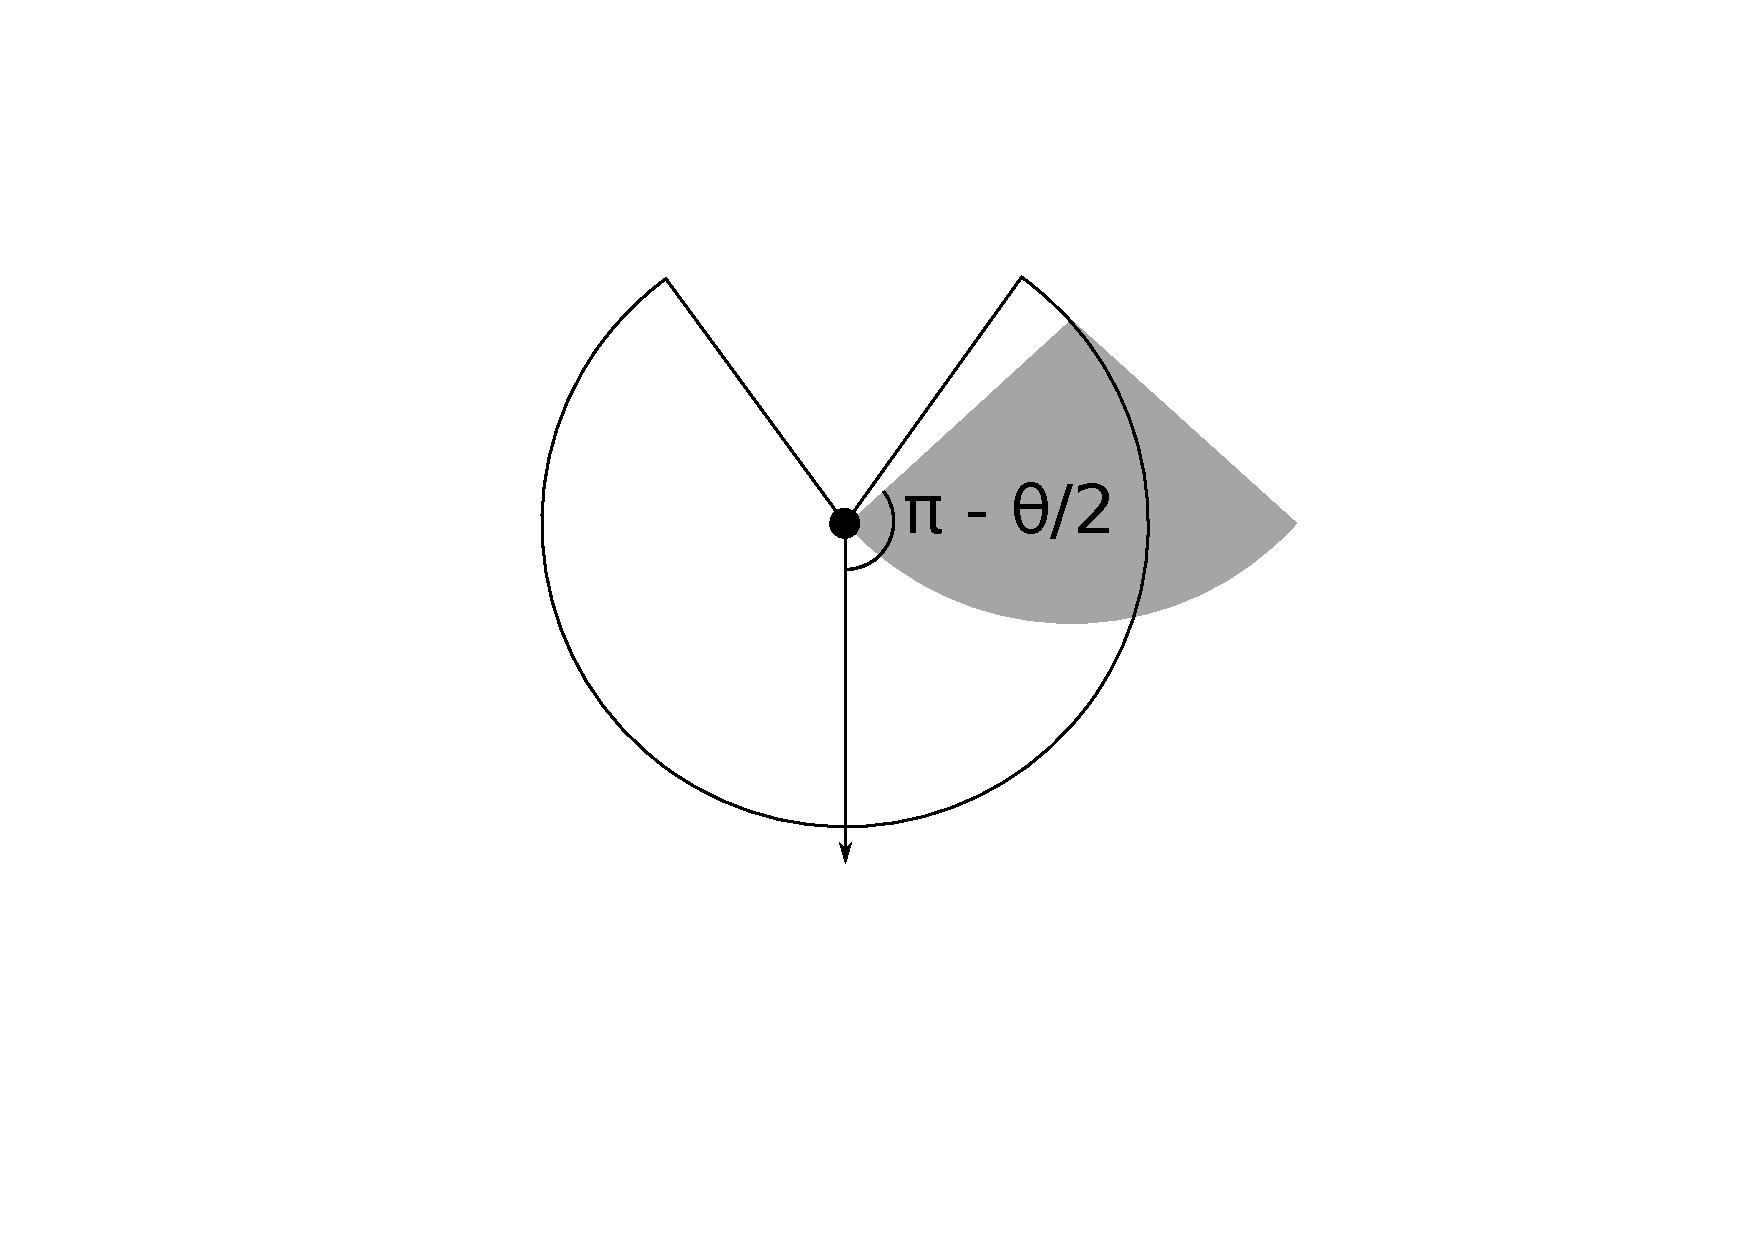
\includegraphics[width=0.45\textwidth, trim=5cm 6cm 4cm 1cm]{imgs/behind2.pdf}      
  }
}
\caption[Profile sizes for an animal approaching from behind: models NW2--4]{
Profile sizes when an animal approaches from behind in models NW2--4.
If $\alpha$ is relatively large, animals can be detected when approaching from behind.
Otherwise animals cannot be detected.
The sector shaped detection region is shown in grey.
Animals are filled black circles and the animal signal is an unfilled sector.
The animals direction of movement is indicated with an arrow.
(a) If $\alpha/2$ is less than $\pi - \theta/2$, as is the case here, then the width of the profile when an animal approaches directly from behind is zero.
(b) If $\alpha/2 > \pi - \theta/2$ the profile width from behind is $2r\sin\left(\theta/2\right)\sin(x_2)$.
}
\label{fig:NW2--4}
\end{figure}


\subsubsection{Model NW2} \label{NW2}

NW2 is bounded by $\alpha \ge 3\pi - 2\theta$, $\alpha \le 2\pi$ and $\theta\le\pi$ (Figure~\ref{fig:equalRegions}).

NW2 has all five profiles as found in NW1.
However, the change from the $r$ profile (third integral) to the $r - r\cos(x_4)$ profile (fourth integral) occurs at $x_4 = 3\pi/2 - \alpha/2$ instead of at $x_4 = \theta$.

\begin{align}
    \bar{p}_{\text{\tiny{NW2}}} =&\frac{1}{\pi} \left(\;\;\int\limits_{\frac{\theta}{2}}^{\frac{\pi}{2}}2 r \sin{\left (\frac{\theta}{2} \right )} \sin{\left (x_{2} \right )}\;\mathrm{d}x_{2}+\int\limits_{0}^{\theta - \frac{\pi}{2}}r - r \cos{\left (- x_{4} + \theta \right )}\;\mathrm{d}x_{4}\right.\notag\\
 &\left.+\int\limits_{\theta - \frac{\pi}{2}}^{\frac{3 \pi}{2} - \frac{\alpha}{2}}r\;\mathrm{d}x_{4}+\int\limits_{\frac{3 \pi}{2} - \frac{\alpha}{2}}^{\theta}r - r \cos{\left (x_{4} \right )}\;\mathrm{d}x_{4}+\int\limits_{\frac{\theta}{2}}^{\frac{\pi}{2}}2 r \sin{\left (\frac{\theta}{2} \right )} \sin{\left (x_{2} \right )}\;\mathrm{d}x_{2}\right)\label{pNW2Def}\\
    \bar{p}_{\text{\tiny{NW2}}}  =& \frac{r}{\pi} \left(\theta - \cos{\left (\frac{\alpha}{2} \right )} + 1\right)\label{pNW2Sln}
\end{align}


\subsubsection{Model NW3} \label{NW3}

NW3 is bounded by $\alpha \le 3\pi - 2\theta$, $\alpha\ge 2\pi-\theta$ and $\theta\ge\pi/2$ (Figure~\ref{fig:equalRegions}).

NW3 does not have the fourth integral from NW2 as animals are not detectable to the right of the sensor until after the $x_4$ region has ended and the $x_2$ region has begun.
Therefore the second $x_4$ integral has an upper limit of $\theta $ and the profile after has a width of $r\cos(x_2 - \theta/2)$ and is integrated with respect to $x_2$.
The final integral starts at $x_4 = 3\pi/2 - \alpha/2 - \theta/2$ and has the full width of $2r\sin(x_2)\sin(\theta/2)$.

\begin{align}
    \bar{p}_{\text{\tiny{NW3}}} =&\frac{1}{\pi} \left(\;\;\int\limits_{\frac{\theta}{2}}^{\frac{\pi}{2}}2 r \sin{\left (\frac{\theta}{2} \right )} \sin{\left (x_{2} \right )}\;\mathrm{d}x_{2}+\int\limits_{0}^{\theta - \frac{\pi}{2}}r - r \cos{\left (- x_{4} + \theta \right )}\;\mathrm{d}x_{4}\right.\notag\\
 &\left.+\int\limits_{\theta - \frac{\pi}{2}}^{\theta}r\;\mathrm{d}x_{4}+\int\limits_{\frac{\theta}{2}}^{\frac{3 \pi}{2} - \frac{\theta}{2} - \frac{\alpha}{2}}r \cos{\left (\frac{\theta}{2} - x_{2} \right )}\;\mathrm{d}x_{2}+\int\limits_{\frac{3 \pi}{2} - \frac{\theta}{2} - \frac{\alpha}{2}}^{\frac{\pi}{2}}2 r \sin{\left (\frac{\theta}{2} \right )} \sin{\left (x_{2} \right )}\;\mathrm{d}x_{2}\right)\label{pNW3Def}\\
    \bar{p}_{\text{\tiny{NW3}}}  =& \frac{r}{\pi} \left(\theta - \cos{\left (\frac{\alpha}{2} \right )} + 1\right)\label{pNW3Sln}
\end{align}

\subsubsection{Model NW4} \label{NW4}

Finally, NW4 is bounded by $\alpha\ge \pi$, $\theta\ge \pi/2$ and $\alpha \le 2\pi - \theta$ (Figure~\ref{fig:equalRegions}).
NW4 is the same as NW3 except that the final profile width is zero and this profile is reached at $\alpha/2+\theta/2-\pi/2$.

\begin{align}
    \bar{p}_{\text{\tiny{NW4}}} =&\frac{1}{\pi} \left(\;\;\int\limits_{\frac{\theta}{2}}^{\frac{\pi}{2}}2 r \sin{\left (\frac{\theta}{2} \right )} \sin{\left (x_{2} \right )}\;\mathrm{d}x_{2}+\int\limits_{0}^{\theta - \frac{\pi}{2}}r - r \cos{\left (- x_{4} + \theta \right )}\;\mathrm{d}x_{4}\right.\notag\\
 &\left.+\int\limits_{\theta - \frac{\pi}{2}}^{\theta}r\;\mathrm{d}x_{4}+\int\limits_{\frac{\theta}{2}}^{\frac{\alpha}{2} + \frac{\theta}{2} - \frac{\pi}{2}}r \cos{\left (\frac{\theta}{2} - x_{2} \right )}\;\mathrm{d}x_{2}\right)\label{pNW4Def}\\
    \bar{p}_{\text{\tiny{NW4}}}  =& \frac{r}{\pi} \left(\theta - \cos{\left (\frac{\alpha}{2} \right )} + 1\right)\label{pNW4Sln}
\end{align}


\subsection{Model REM} \label{REM}

REM is the model from \cite{rowcliffe2008estimating}.
It has $\alpha =2\pi$ and $\theta \le \pi/2$ (Figure~\ref{fig:equalRegions}).
It has three profile widths, two of which are repeated, once as the animal approaches from in front of the sensor and once as the animal approaches from behind the sensor.

\begin{enumerate}
\item Starting with an approach direction of directly towards the sensor, and examining focal angle $x_2$, the profile width is $2r\sin(x_2)\sin(\theta/2)$.
\item When the profile is perpendicular to the radius on the right hand of the sector sensor region, we instead examine $x_3$ where the profile width is $r\sin(x_3)$.
\item At $x_3=\pi/2$ the profile becomes simply $r$ and this continues for $\theta $ radians of $x_4$.
\item The $x_3$ profile is then repeated with an approach direction from behind the sensor.
\item Finally the $x_2$ profile is repeated, again with an approach direction from behind the sensor.
\end{enumerate}

\begin{align}
    \bar{p}_{\text{\tiny{REM}}} =&\frac{1}{\pi} \left(\;\;\int\limits_{\frac{\pi}{2} - \frac{\theta}{2}}^{\frac{\pi}{2}}2 r \sin{\left (\frac{\theta}{2} \right )} \sin{\left (x_{2} \right )}\;\mathrm{d}x_{2}+\int\limits_{\theta}^{\frac{\pi}{2}}r \sin{\left (x_{3} \right )}\;\mathrm{d}x_{3}\right.\notag\\
 &\left.+\int\limits_{0}^{\theta}r\;\mathrm{d}x_{4}+\int\limits_{\theta}^{\frac{\pi}{2}}r \sin{\left (x_{3} \right )}\;\mathrm{d}x_{3}+\int\limits_{\frac{\pi}{2} - \frac{\theta}{2}}^{\frac{\pi}{2}}2 r \sin{\left (\frac{\theta}{2} \right )} \sin{\left (x_{2} \right )}\;\mathrm{d}x_{2}\right)\label{pREMDef}\\
    \bar{p}_{\text{\tiny{REM}}}  =& \frac{r}{\pi} \left(\theta + 2\right)\label{pREMSln}
\end{align}

\subsection{Models NW5--7} \label{NW57}

In the models NW5--7, the sensor has $\theta \le \pi/2$ as in the REM.
As $\alpha \ge \pi$ a lot of the profiles are similar to the REM.
Specifically, the first three profiles are always the same as the first three profiles of the REM.
This is because when an animal is moving towards the sensor, the $\alpha \ge \pi$ signal is no different to a $2\pi$ signal.
However, when approaching the sensor from behind, things are slightly different.
The animal can only be detected by the sensor if the signal width is large enough that it can be detected once it has passed the sensor.
                    
\begin{enumerate}
\item Starting with an approach direction of directly towards the sensor, and examining focal angle $x_2$, the profile width is $2r\sin(x_2)\sin(\theta/2)$.
\item When the profile is perpendicular to the radius edge of the sector sensor region, we instead examine $x_3$ where the profile width is $r\sin(x_3)$.
\item At $x_3=\pi/2$ the profile becomes simply $r$ and this continues for $\theta $ radians of $x_4$.
\item If $\alpha \le 2\pi + 2\theta$, the animal becomes undetectable during this profile when  $x_3$ has decreased in size to $\pi - \alpha/2$.
This inequality marks the boundary between NW7 and NW6.
\item If instead $\alpha \ge 2\pi + 2\theta$ then the animal does not become undetectable during the $x_3$ focal angle.
Instead the profile has width greater than zero for the whole of the $x_3$ angle.
The $x_2$ profile starts with width $r\cos(x_2 - \theta/2)$ as only animals approaching to the left of the sensor are detectable.
\item During this second $x_2$ profile the signal width needed for animals to be detected to the left of the detector is increasing while the angle needed for animals to be detected to the right of the detector is decreasing.
Therefore, either the left side becomes undetectable, making both sides undetectable (this occurs if $\alpha \le 2\pi - \theta$ as in NW6) \item or the right becomes detectable (if $\alpha \ge 2\pi - \theta$ as in NW5), making both sides detectable and giving a profile width of $2r\sin(x_2)\sin(\theta/2)$.
\end{enumerate}


\subsubsection{Model NW5} \label{NW5}

NW5 is bounded by $\alpha \ge 2\pi - \theta$, $\alpha \le 2\pi$ and $\theta \le \pi/2$ (Figure~\ref{fig:equalRegions}).

It is the same as REM except that it includes the extra profile in $x_2$ (the fifth integral) where only animals approaching to the left of the profile are detected.

\begin{align}
    \bar{p}_{\text{\tiny{NW5}}} =&\frac{1}{\pi} \left(\;\;\int\limits_{\frac{\pi}{2} - \frac{\theta}{2}}^{\frac{\pi}{2}}2 r \sin{\left (\frac{\theta}{2} \right )} \sin{\left (x_{2} \right )}\;\mathrm{d}x_{2}+\int\limits_{\theta}^{\frac{\pi}{2}}r \sin{\left (x_{3} \right )}\;\mathrm{d}x_{3}+\int\limits_{0}^{\theta}r\;\mathrm{d}x_{4}\right.\notag\\
 &\left.+\int\limits_{\theta}^{\frac{\pi}{2}}r \sin{\left (x_{3} \right )}\;\mathrm{d}x_{3}+\int\limits_{\frac{\pi}{2} - \frac{\theta}{2}}^{\frac{3 \pi}{2} - \frac{\theta}{2} - \frac{\alpha}{2}}r \cos{\left (\frac{\theta}{2} - x_{2} \right )}\;\mathrm{d}x_{2}+\int\limits_{\frac{3 \pi}{2} - \frac{\theta}{2} - \frac{\alpha}{2}}^{\frac{\pi}{2}}2 r \sin{\left (\frac{\theta}{2} \right )} \sin{\left (x_{2} \right )}\;\mathrm{d}x_{2}\right)\label{pNW5Def}\\
    \bar{p}_{\text{\tiny{NW5}}}  =& \frac{r}{\pi} \left(\theta - \cos{\left (\frac{\alpha}{2} \right )} + 1\right)\label{pNW5Sln}
\end{align}

\subsubsection{Model NW6} \label{NW6}

NW6 is bounded by $\alpha \le 2\pi - \theta$, $\alpha \ge 2\pi + 2\theta$ and $\theta \le \pi/2$ (Figure~\ref{fig:equalRegions}).

NW6 is the same NW5 except that as $\alpha \le 2\pi - \theta$, animals that approach from directly behind the detector are not detected.
Therefore at $x_2 = \alpha/2 + \theta/2 - \pi/2$ the profile width goes to zero and therefore the last integral in NW5 is not included.

\begin{align}
    \bar{p}_{\text{\tiny{NW6}}} =&\frac{1}{\pi} \left(\;\;\int\limits_{\frac{\pi}{2} - \frac{\theta}{2}}^{\frac{\pi}{2}}2 r \sin{\left (\frac{\theta}{2} \right )} \sin{\left (x_{2} \right )}\;\mathrm{d}x_{2}+\int\limits_{\theta}^{\frac{\pi}{2}}r \sin{\left (x_{3} \right )}\;\mathrm{d}x_{3}\right.\notag\\
 &\left.+\int\limits_{0}^{\theta}r\;\mathrm{d}x_{4}+\int\limits_{\theta}^{\frac{\pi}{2}}r \sin{\left (x_{3} \right )}\;\mathrm{d}x_{3}+\int\limits_{\frac{\pi}{2} - \frac{\theta}{2}}^{\frac{\alpha}{2} + \frac{\theta}{2} - \frac{\pi}{2}}r \cos{\left (\frac{\theta}{2} - x_{2} \right )}\;\mathrm{d}x_{2}\right)\label{pNW6Def}\\
    \bar{p}_{\text{\tiny{NW6}}}  =& \frac{r}{\pi} \left(\theta - \cos{\left (\frac{\alpha}{2} \right )} + 1\right)\label{pNW6Sln}
\end{align}



\subsubsection{Model NW7} \label{NW7}

NW7 is bounded by $\alpha \ge 2\pi + 2\theta$, $\alpha \ge \pi$ and $\theta \ge 0$ (Figure~\ref{fig:equalRegions}).

It is similar to NW6 but does not include the last integral as during the $x_3$ profile, at $x_3 = \pi - \alpha/2$ the signal width is too small for any animals to be detected, so the profile width goes to zero.

\begin{align}
    \bar{p}_{\text{\tiny{NW7}}} =&\frac{1}{\pi} \left(\;\;\int\limits_{\frac{\pi}{2} - \frac{\theta}{2}}^{\frac{\pi}{2}}2 r \sin{\left (\frac{\theta}{2} \right )} \sin{\left (x_{2} \right )}\;\mathrm{d}x_{2}+\int\limits_{\theta}^{\frac{\pi}{2}}r \sin{\left (x_{3} \right )}\;\mathrm{d}x_{3}\right.\notag\\
 &\left.+\int\limits_{0}^{\theta}r\;\mathrm{d}x_{4}+\int\limits_{\pi - \frac{\alpha}{2}}^{\frac{\pi}{2}}r \sin{\left (x_{3} \right )}\;\mathrm{d}x_{3}\right)\label{pNW7Def}\\
    \bar{p}_{\text{\tiny{NW7}}}  =& \frac{r}{\pi} \left(\theta - \cos{\left (\frac{\alpha}{2} \right )} + 1\right)\label{pNW7Sln}
\end{align}





\subsection{Model SW1--3} \label{SW13}
 
The models in SW1--3 are described with the two focal angles used in models NW2--4, $x_2$ and $x_4$.
As $\alpha \le\pi$ an animal can never be detected if it is approaching the detector from behind.
This makes these models simpler in that they go through the $x_2$ and $x_4$ profiles only once each.

\begin{figure}[t]
  \centering
{
  \subfloat[\label{fig:SWforward}]{
    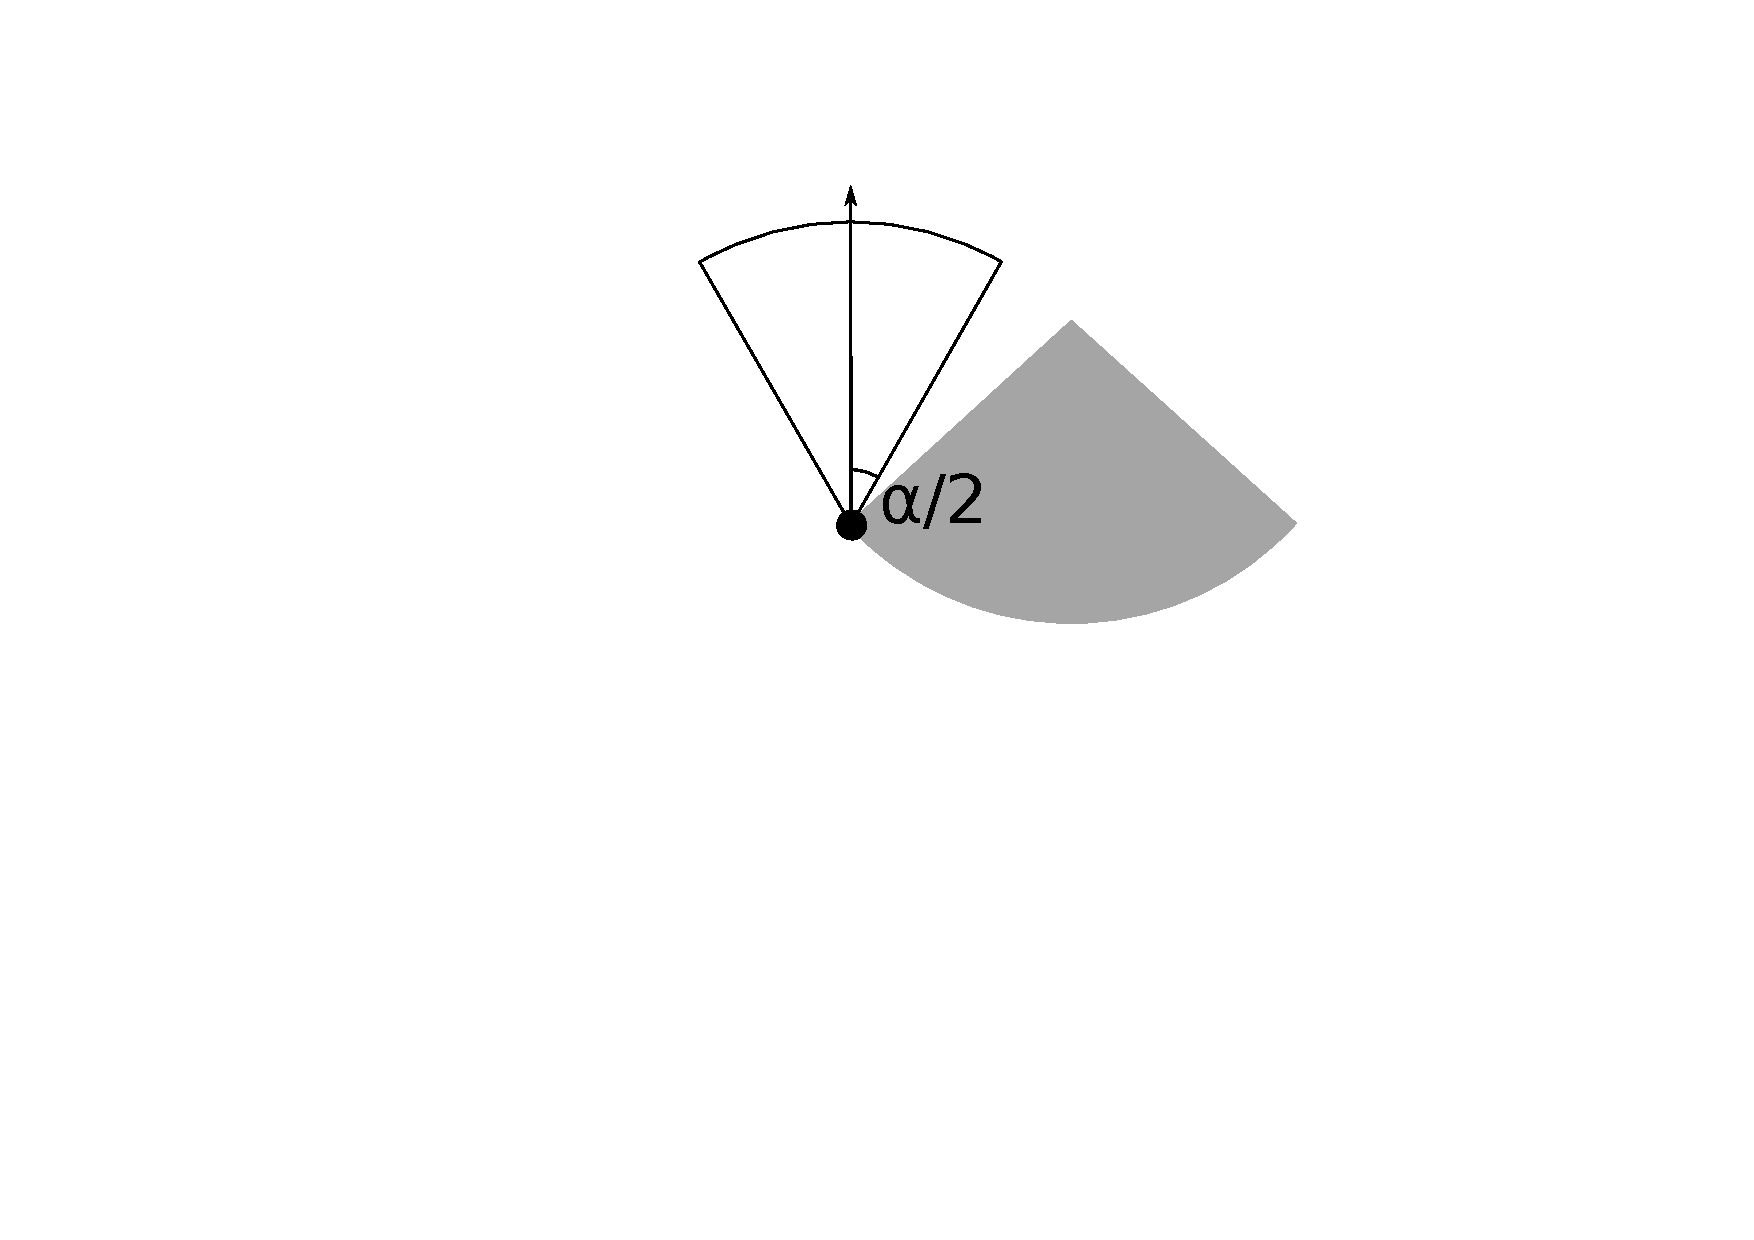
\includegraphics[width=0.45\textwidth, trim=7cm 10cm 6cm 1cm]{imgs/forward.pdf}
  }
  \subfloat[\label{fig:SWforwad2}]{
    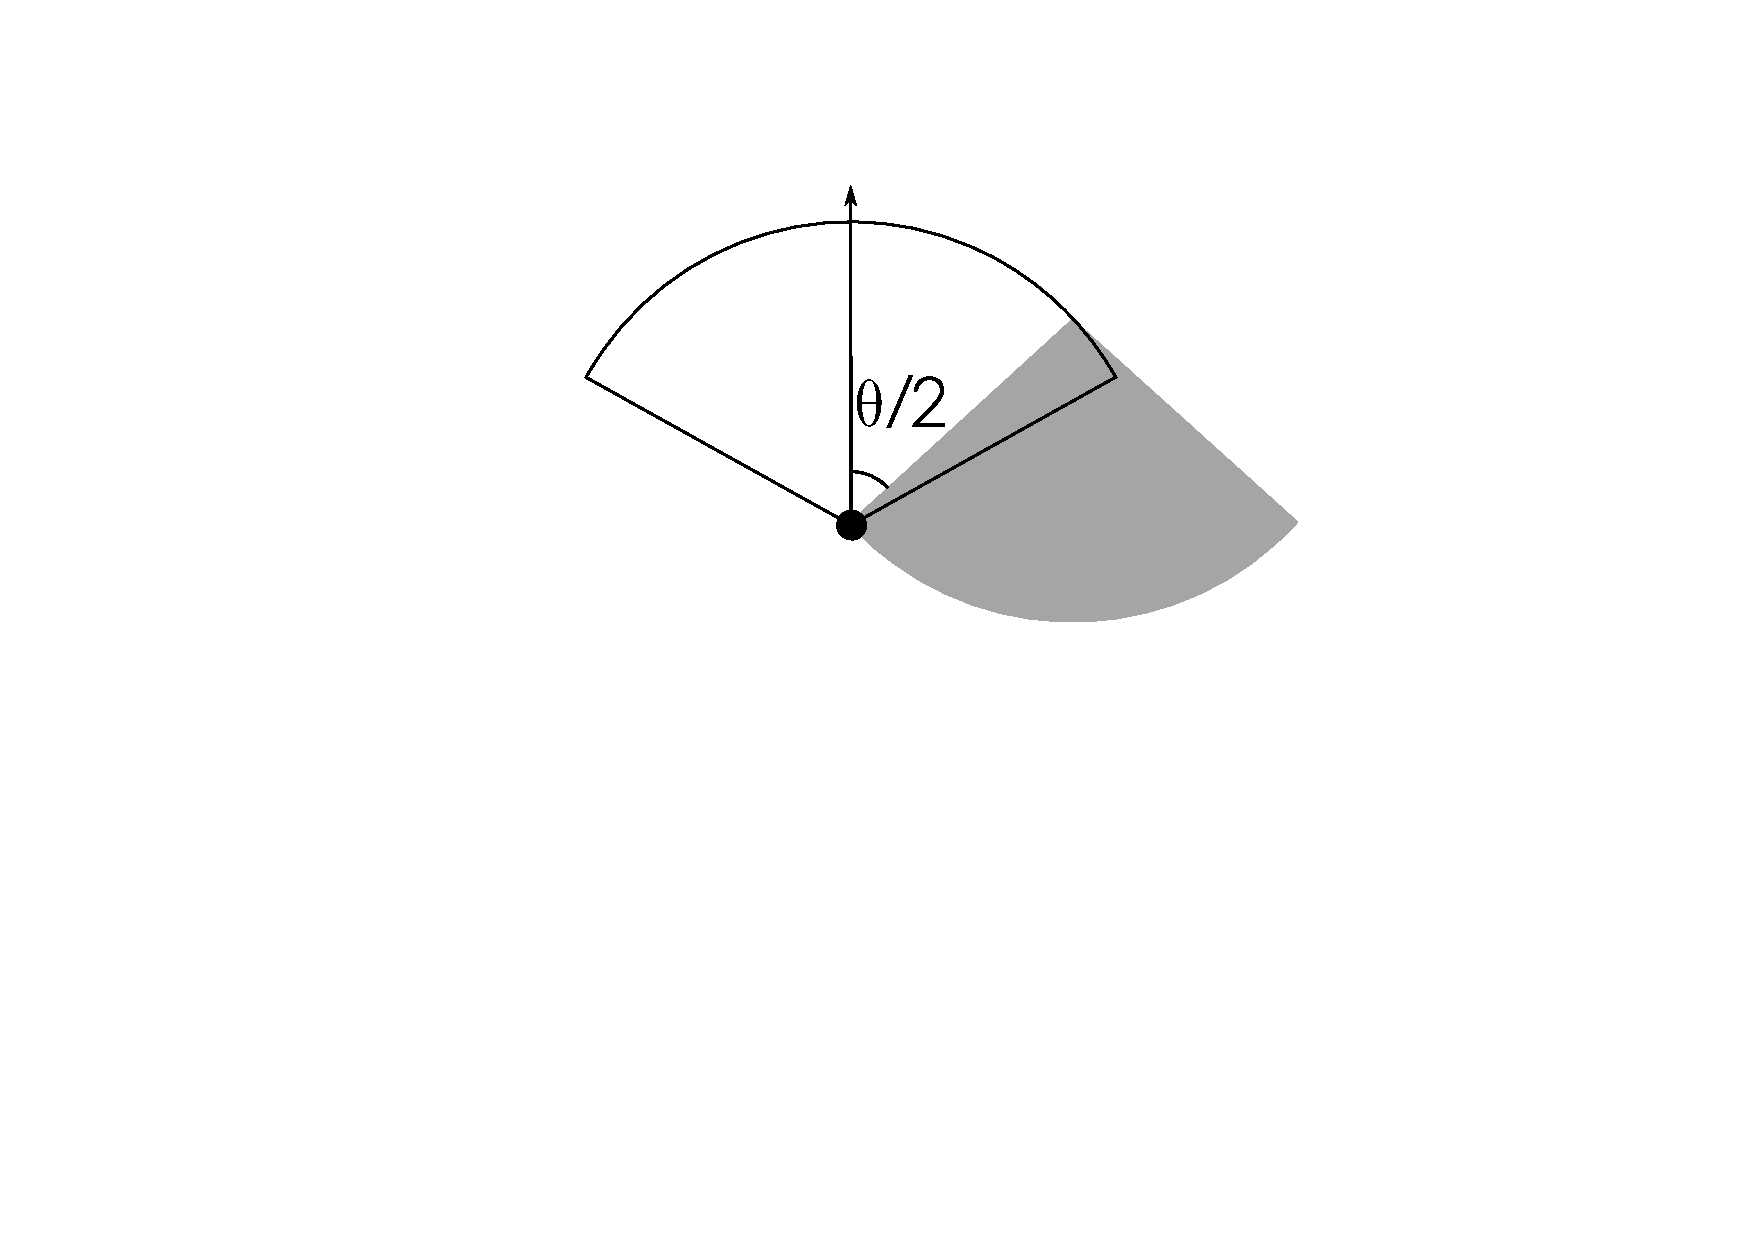
\includegraphics[width=0.45\textwidth, trim=7cm 10cm 6cm 1cm]{imgs/forward2.pdf}
  }
}
\caption[The first profile in SW models]{
The first profile in SW models is limited by either $\alpha$ or $\beta$ depending on whether $\alpha < \beta$.
The sector shaped detection region is shown in grey.
Animals are filled black circles and the animal signal is an unfilled sector.
The animals direction of movement is indicated with an arrow.
(a)  As $\alpha/2 < \theta/2$ the profile width is limited by the signal width rather than the sensor region.
The profile width is $2r\sin\left(\alpha/2\right)$ (b) As $\alpha/2 > \theta/2$ the profile width is limited by the sensor region, not the signal width.
The profile width is $2r\sin\left(\theta/2\right)\sin(x_2)$.
}
\label{fig:forward}
\end{figure}


There are five potential profile sizes.
\begin{enumerate}
\item At the beginning of $x_2$, with an approach direction directly towards the sensor, the parameter that limits the width of the profile can either be the sensor width,  in which case the profile width is $2r\sin\left(\theta/2\right)\sin(x_2)$.
\item Or the signal width can be the limiting parameter, in which case the profile width is instead $2r\sin(\alpha /2)$ (Figure~\ref{fig:forward})
\item The next potential profile in $x_2$ has a width of $r\sin(\alpha/2) - r\cos(x_2 + \theta/2)$ as the right side of the profile is limited by the width of the sensor region while the left side is limited by the signal width.
However, the angle at which the profile starts depends on whether the first profile was 1) or 2) above.
If the first profile is profile 1) then the profile is limited on both sides by the sensor region and then the left side of the profile becomes limited by the signal width.
This happens at $x_2 = \pi/2 - \alpha/2 + \theta/2$.
If however the first profile was 2) then the first profile is limited by the signal width.
We move into the new profile when the right side of the profile becomes limited by the sensor region.
This occurs at $x_2 = \pi/2 + \alpha/2 - \theta/2$.


\item In the $x_4$ region the left side of the profile is always $r\sin(\alpha /2)$ while the right side is either 0, giving a profile of $r\sin(\alpha /2)$.

\item Or limited by the sensor giving a profile of size $r\sin (\alpha /2) -r\cos(x_4-\theta) $.
\end{enumerate}

\subsubsection{Model SW1} \label{SW1}

SW1 is bounded by $\alpha \ge \theta$, $\alpha \le\pi$ and $\theta \le \pi$ (Figure~\ref{fig:equalRegions}).

As $\alpha $ is large the first profile is limited by the size of the sensor region giving it a width of $2r\sin\left(\theta/2\right)\sin(x_2)$.
It is the only one of the three SW models to start in this way.
Later on, still with $x_2$ as the focal angle the left side of the profile does become limited by the signal width.
So at $x_2= \pi/2 - \alpha/2 + \theta/2$ the profile width becomes $r\sin(\alpha/2) - r\cos(x_2 + \theta/2)$.

As we enter the $x_4$ region, the profile remains limited by the signal on the left and by the sensor on the right, giving a profile width of  $r\sin (\alpha /2) -r\cos(x_4-\theta) $.
Finally, at $x_4 = \theta - \pi/2$ the right side of the profile becomes zero and the profile is width is $r\sin(\alpha /2)$.

\begin{align}
    \bar{p}_{\text{\tiny{SW1}}} =&\frac{1}{\pi} \left(\;\;\int\limits_{\frac{\pi}{2} + \frac{\theta}{2} - \frac{\alpha}{2}}^{\frac{\pi}{2}}2 r \sin{\left (\frac{\theta}{2} \right )} \sin{\left (x_{2} \right )}\;\mathrm{d}x_{2}+\int\limits_{\frac{\theta}{2}}^{\frac{\pi}{2} + \frac{\theta}{2} - \frac{\alpha}{2}}r \sin{\left (\frac{\alpha}{2} \right )} - r \cos{\left (\frac{\theta}{2} + x_{2} \right )}\;\mathrm{d}x_{2}\right.\notag\\
 &\left.+\int\limits_{0}^{\theta - \frac{\pi}{2}}r \sin{\left (\frac{\alpha}{2} \right )} - r \cos{\left (\theta - x_{4} \right )}\;\mathrm{d}x_{4}+\int\limits_{\theta - \frac{\pi}{2}}^{\frac{\alpha}{2} + \theta - \frac{\pi}{2}}r \sin{\left (\frac{\alpha}{2} \right )}\;\mathrm{d}x_{4}\right)\label{pSW1Def}\\
    \bar{p}_{\text{\tiny{SW1}}}  =& \frac{r}{\pi} \left(\theta \sin{\left (\frac{\alpha}{2} \right )} - \cos{\left (\frac{\alpha}{2} \right )} + 1\right)\label{pSW1Sln}
\end{align}

\subsubsection{Model SW2} \label{SW2}

SW2 is bounded by $\theta \ge \pi/2$, $\alpha \le \theta$ and $\alpha \ge 2\theta -\pi$ (Figure~\ref{fig:equalRegions}).

SW2 is largely similar to SW1.
However, as $\alpha \le \theta$ the first profile is limited by $\alpha$ and not by the detection region.
Therefore the first profile has width $2r\sin(\alpha /2)$.
This also means the transition to the second profile occurs at  $x_2 = \pi/2 + \alpha/2 - \theta/2$ instead of  $x_2 = \pi/2 - \alpha/2 + \theta/2$.

\begin{align}
    \bar{p}_{\text{\tiny{SW2}}} =&\frac{1}{\pi} \left(\;\;\int\limits_{\frac{\alpha}{2} - \frac{\theta}{2} + \frac{\pi}{2}}^{\frac{\pi}{2}}2 r \sin{\left (\frac{\alpha}{2} \right )}\;\mathrm{d}x_{2}+\int\limits_{\frac{\theta}{2}}^{\frac{\alpha}{2} - \frac{\theta}{2} + \frac{\pi}{2}}r \sin{\left (\frac{\alpha}{2} \right )} - r \cos{\left (\frac{\theta}{2} + x_{2} \right )}\;\mathrm{d}x_{2}\right.\notag\\
 &\left.+\int\limits_{0}^{\theta - \frac{\pi}{2}}r \sin{\left (\frac{\alpha}{2} \right )} - r \cos{\left (\theta - x_{4} \right )}\;\mathrm{d}x_{4}+\int\limits_{\theta - \frac{\pi}{2}}^{\frac{\alpha}{2} + \theta - \frac{\pi}{2}}r \sin{\left (\frac{\alpha}{2} \right )}\;\mathrm{d}x_{4}\right)\label{pSW2Def}\\
    \bar{p}_{\text{\tiny{SW2}}}  =& \frac{r}{\pi} \left(\theta \sin{\left (\frac{\alpha}{2} \right )} - \cos{\left (\frac{\alpha}{2} \right )} + 1\right)\label{pSW2Sln}
\end{align}



\subsubsection{Model SW3} \label{SW3}

SW3 is bounded by $\alpha \le 2\theta -\pi$ and $\theta \le \pi$ (Figure~\ref{fig:equalRegions}).

SW3 is similar to SW2 except that the profile does not become limited by sensor at all during the the $x_4$ regions.
Therefore, at $x_4 = 0 $ the profile is still of width $2r\sin(\alpha /2)$.
Only at $x_4 = \theta - \pi/2 - \alpha/2$ does the profile become limited on the right by the sensor region.

\begin{align}
    \bar{p}_{\text{\tiny{SW3}}} =&\frac{1}{\pi} \left(\;\;\int\limits_{\frac{\theta}{2}}^{\frac{\pi}{2}}2 r \sin{\left (\frac{\alpha}{2} \right )}\;\mathrm{d}x_{2}+\int\limits_{0}^{- \frac{\pi}{2} + \theta - \frac{\alpha}{2}}2 r \sin{\left (\frac{\alpha}{2} \right )}\;\mathrm{d}x_{4}\right.\notag\\
 &\left.+\int\limits_{- \frac{\pi}{2} + \theta - \frac{\alpha}{2}}^{\theta - \frac{\pi}{2}}r \sin{\left (\frac{\alpha}{2} \right )} - r \cos{\left (\theta - x_{4} \right )}\;\mathrm{d}x_{4}+\int\limits_{\theta - \frac{\pi}{2}}^{\frac{\alpha}{2} + \theta - \frac{\pi}{2}}r \sin{\left (\frac{\alpha}{2} \right )}\;\mathrm{d}x_{4}\right)\label{pSW3Def}\\
    \bar{p}_{\text{\tiny{SW3}}}  =& \frac{r}{\pi} \left(\theta \sin{\left (\frac{\alpha}{2} \right )} - \cos{\left (\frac{\alpha}{2} \right )} + 1\right)\label{pSW3Sln}
\end{align}


\subsection{Model SW4--9} \label{SW4--9}

As $\alpha < \pi$, animals approaching the sensor from behind can never be detected, so unlike REM, the second $x_2$ and $x_3$ profiles are always zero.
The six models are split by three inequalities that relate to the models as follows.

\begin{enumerate}
\item Models with $\alpha \le \pi - 2\theta$  have no $x_4$ profile.
This is because at $x_4 = 0$, the signal width is already too small to be detected as can be seen in Figure~\ref{fig:SW4--9nox4} where $\alpha/2 < \pi/2 - \theta$ which simplifies to give the previous inequality.

\item Models with $\alpha \le \theta$ are limited by $\alpha$ in the first, $x_2$ region (Figure~\ref{fig:forward}), rather than being limited by $\theta$.
Therefore this first profile is of width $2r\sin(\alpha/2)$ rather than $2r\sin(\theta/2)\sin(x_2)$.

\item Finally, models with $\alpha \le 2\theta$ have a second profile in $x_2$ where to one side of the sensor $\alpha$ is the limiting factor of profile width, while on the other side $\theta$ is (Figure~\ref{fig:4--9int3}).
This gives a width of $r\sin(\alpha/2) - r\cos(x_2 + \theta/2)$.
This profile does not occur in models with $\alpha \ge 2\theta$.

\end{enumerate}

\begin{figure}[t]
 \centering
{
  \subfloat[\label{fig:SW4--9nox4}]{
    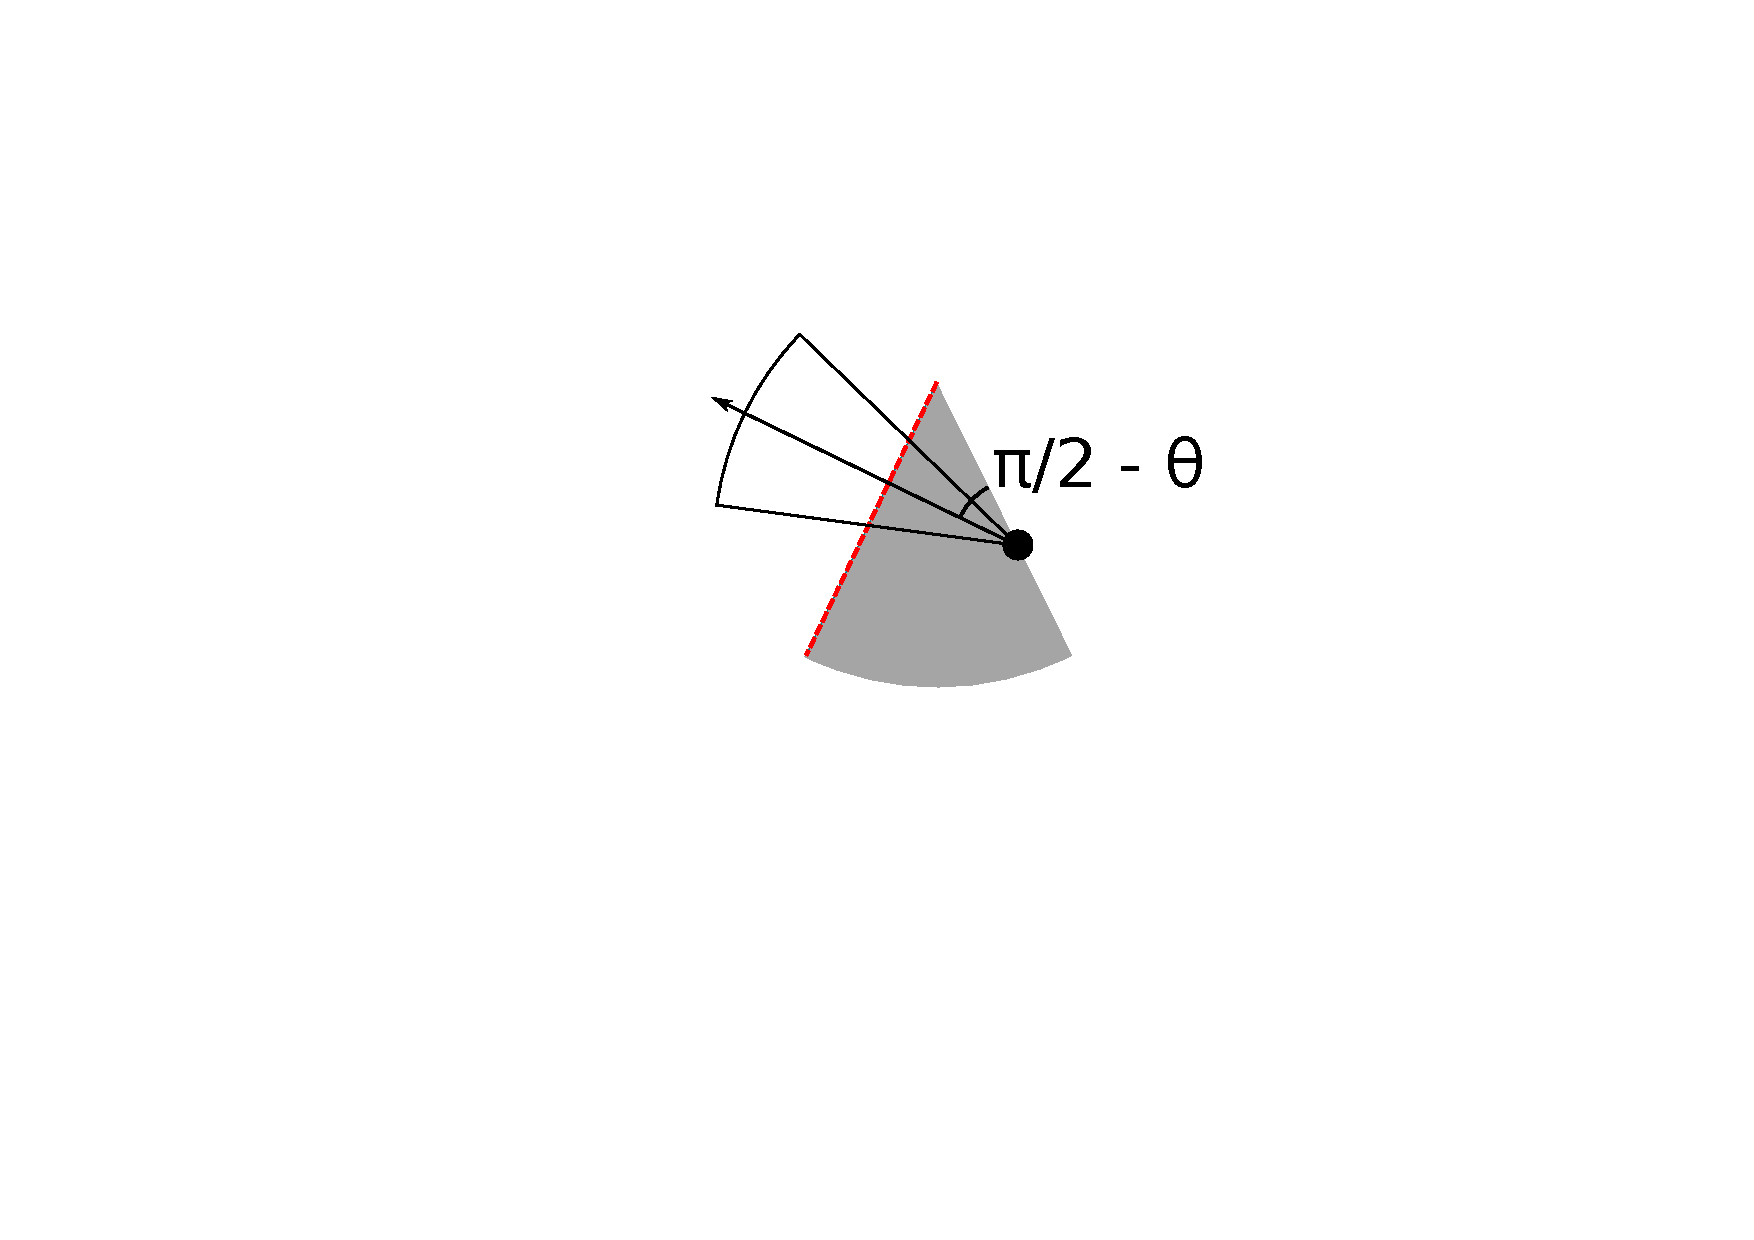
\includegraphics[width=.5\textwidth, trim=8cm 9cm 8cm 4cm]{imgs/x4is0.pdf}
  }
  \subfloat[\label{fig:4--9int3}]{
    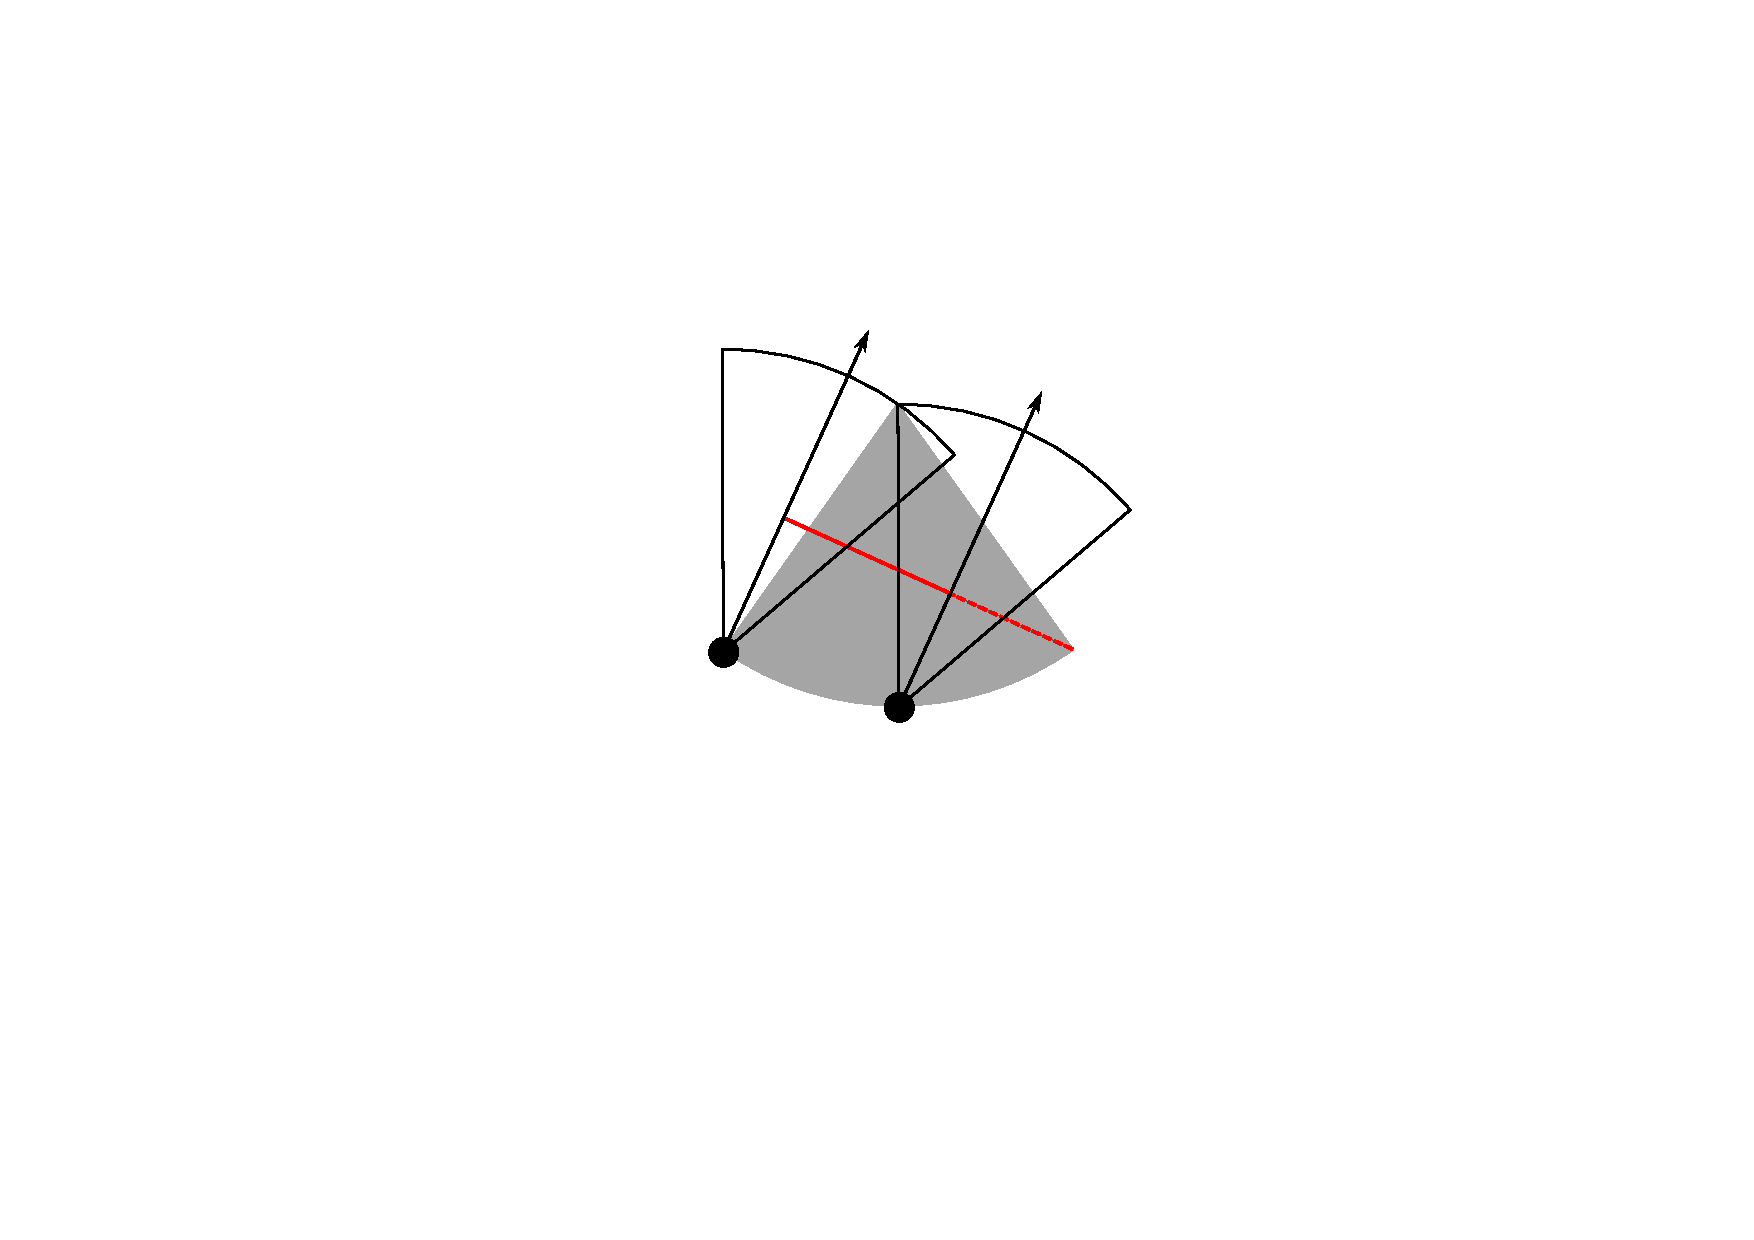
\includegraphics[width=.5\textwidth, trim=8cm 9cm 8cm 4cm]{imgs/4--9int3.pdf}
  }
}
\caption[Description of two profiles in SW models]{
Description of two profiles in SW models.
The sector shaped detection region is shown in grey.
Animals are filled black circles and the animal signal is an unfilled sector.
The animals direction of movement is indicated with an arrow.
The profile $p$ is shown with a red line.
Dashed red lines indicate areas where animals cannot be detected.
(a) At $x_4 = 0$, if $\alpha/2 < \pi/2 - \theta$ then $\alpha/2$ is too small for an animal to be detected at all during the $x_4$ profile (shown with dashed red).
This inequality simplifies to $\alpha < \pi - 2\theta$.
(b) The right of the profile is limited by the signal width, not the sensor.
On the left, the profile is limited by the sensor and not the signal.
Overall the profile width is $r\sin(\alpha/2) - r\cos(x_2 + \theta/2)$.
}
\label{fig:SW4--9}
\end{figure}

\subsubsection{Model SW4} \label{SW4}

SW4 is bounded by $\alpha \le \theta$, $\alpha \ge \pi - 2\theta$ and $\theta \le \pi/2$ (Figure~\ref{fig:equalRegions}).
Therefore it does contain a $x_4$ profile, starts with an $\alpha$ limited profile and does contain the $r\sin(\alpha/2) - r\cos(x_2 + \theta/2)$ profile in $x_2$.

\begin{align}
    \bar{p}_{\text{\tiny{SE4}}} =&\frac{1}{\pi} \left(\;\;\int\limits_{\frac{\pi}{2}}^{\frac{\pi}{2} + \frac{\theta}{2} - \frac{\alpha}{2}}2 r \sin{\left (\frac{\alpha}{2} \right )}\;\mathrm{d}x_{1}+\int\limits_{\frac{\pi}{2} + \frac{\theta}{2} - \frac{\alpha}{2}}^{\frac{\theta}{2} + \frac{\pi}{2}}r \sin{\left (\frac{\alpha}{2} \right )} + r \cos{\left (\frac{\theta}{2} - x_{1} \right )}\;\mathrm{d}x_{1}\right.\notag\\
 &\left.+\int\limits_{\frac{\theta}{2} + \frac{\pi}{2}}^{\frac{\alpha}{2} + \frac{\theta}{2} + \frac{\pi}{2}}r \sin{\left (\frac{\alpha}{2} \right )}\;\mathrm{d}x_{1}\right)\label{pSW4Def}\\
    \bar{p}_{\text{\tiny{SE4}}}  =& \frac{r}{\pi} \left(\theta \sin{\left (\frac{\alpha}{2} \right )} - \cos{\left (\frac{\alpha}{2} \right )} + 1\right)\label{pSW4Sln}
\end{align}


\subsubsection{Model SW5} \label{SW5}

SW5 is the only model with a tetrahedral bounding region.
It is bounded by $\alpha \ge \theta$, $\alpha \ge \pi - 2\theta$, $\alpha \le 2\theta$ and $\theta \le \pi/2$ (Figure~\ref{fig:equalRegions}).
Therefore it does contain a $x_4$ profile, but starts with a $\theta$ limited profile.
It does contain the $r\sin(\alpha/2) - r\cos(x_2 + \theta/2)$ profile in $x_2$.

\begin{align}
    \bar{p}_{\text{\tiny{SW5}}} =&\frac{1}{\pi} \left(\;\;\int\limits_{\frac{\pi}{2} + \frac{\theta}{2} - \frac{\alpha}{2}}^{\frac{\pi}{2}}2 r \sin{\left (\frac{\theta}{2} \right )} \sin{\left (x_{2} \right )}\;\mathrm{d}x_{2}+\int\limits_{\frac{\pi}{2} - \frac{\theta}{2}}^{\frac{\pi}{2} + \frac{\theta}{2} - \frac{\alpha}{2}}r \sin{\left (\frac{\alpha}{2} \right )} - r \cos{\left (\frac{\theta}{2} + x_{2} \right )}\;\mathrm{d}x_{2}\right.\notag\\
 &\left.+\int\limits_{\theta}^{\frac{\pi}{2}}r \sin{\left (\frac{\alpha}{2} \right )}\;\mathrm{d}x_{3}+\int\limits_{0}^{\frac{\alpha}{2} + \theta - \frac{\pi}{2}}r \sin{\left (\frac{\alpha}{2} \right )}\;\mathrm{d}x_{4}\right)\label{pSW5Def}\\
    \bar{p}_{\text{\tiny{SW5}}}  =& \frac{r}{\pi} \left(\theta \sin{\left (\frac{\alpha}{2} \right )} - \cos{\left (\frac{\alpha}{2} \right )} + 1\right)\label{pSW5Sln}
\end{align}

\subsubsection{Model SW6} \label{SW6}

SW6 is bounded by $\alpha \ge \pi - 2\theta$,  $\alpha \ge 2\theta$ and $\alpha \le \pi$ (Figure~\ref{fig:equalRegions}).
It starts with a $\theta$ limited profile and has a $x_4$ profile.
However, it does not contain the $r\sin(\alpha/2) - r\cos(x_2 + \theta/2)$ profile.

\begin{align}
    \bar{p}_{\text{\tiny{SW6}}} =&\frac{1}{\pi} \left(\;\;\int\limits_{\frac{\pi}{2} - \frac{\theta}{2}}^{\frac{\pi}{2}}2 r \sin{\left (\frac{\theta}{2} \right )} \sin{\left (x_{2} \right )}\;\mathrm{d}x_{2}+\int\limits_{\theta}^{\frac{\alpha}{2}}r \sin{\left (x_{3} \right )}\;\mathrm{d}x_{3}\right.\notag\\
 &\left.+\int\limits_{\frac{\alpha}{2}}^{\frac{\pi}{2}}r \sin{\left (\frac{\alpha}{2} \right )}\;\mathrm{d}x_{3}+\int\limits_{0}^{\frac{\alpha}{2} + \theta - \frac{\pi}{2}}r \sin{\left (\frac{\alpha}{2} \right )}\;\mathrm{d}x_{4}\right)\label{pSW6Def}\\
    \bar{p}_{\text{\tiny{SW6}}}  =& \frac{r}{\pi} \left(\theta \sin{\left (\frac{\alpha}{2} \right )} - \cos{\left (\frac{\alpha}{2} \right )} + 1\right)\label{pSW6Sln}
\end{align}


\subsubsection{Model SW7} \label{SW7}

SW7 is bounded by $\alpha \le \pi - 2\theta$, $\alpha \le \theta$ and $\alpha < 0$ (Figure~\ref{fig:equalRegions}).
Therefore it does not contain a $x_4$ profile.
It starts with an $\alpha$ limited profile and contains the $r\sin(\alpha/2) - r\cos(x_2 + \theta/2)$ profile in $x_2$.


\begin{align}
    \bar{p}_{\text{\tiny{SW7}}} =&\frac{1}{\pi} \left(\;\;\int\limits_{\frac{\alpha}{2} - \frac{\theta}{2} + \frac{\pi}{2}}^{\frac{\pi}{2}}2 r \sin{\left (\frac{\alpha}{2} \right )}\;\mathrm{d}x_{2}+\int\limits_{\frac{\pi}{2} - \frac{\theta}{2}}^{\frac{\alpha}{2} - \frac{\theta}{2} + \frac{\pi}{2}}r \sin{\left (\frac{\alpha}{2} \right )} - r \cos{\left (\frac{\theta}{2} + x_{2} \right )}\;\mathrm{d}x_{2}+\int\limits_{\theta}^{\frac{\alpha}{2} + \theta}r \sin{\left (\frac{\alpha}{2} \right )}\;\mathrm{d}x_{3}\right)\label{pSW7Def}\\
    \bar{p}_{\text{\tiny{SW7}}}  =& \frac{r}{\pi} \left(\theta \sin{\left (\frac{\alpha}{2} \right )} - \cos{\left (\frac{\alpha}{2} \right )} + 1\right)\label{pSW7Sln}
\end{align}

\subsubsection{Model SW8} \label{SW8}

SW8 is bounded by $\alpha \le \pi - 2\theta$, $\alpha \ge \theta$ and $\alpha \le 2\theta$ (Figure~\ref{fig:equalRegions}).
It starts with a $\theta$ limited profile.
It does contain the $r\sin(\alpha/2) - r\cos(x_2 + \theta/2)$ profile in $x_2$ but does not have a $x_4$ profile.

\begin{align}
    \bar{p}_{\text{\tiny{SW8}}} =&\frac{1}{\pi} \left(\;\;\int\limits_{\frac{\pi}{2} + \frac{\theta}{2} - \frac{\alpha}{2}}^{\frac{\pi}{2}}2 r \sin{\left (\frac{\theta}{2} \right )} \sin{\left (x_{2} \right )}\;\mathrm{d}x_{2}+\int\limits_{\frac{\pi}{2} - \frac{\theta}{2}}^{\frac{\pi}{2} + \frac{\theta}{2} - \frac{\alpha}{2}}r \sin{\left (\frac{\alpha}{2} \right )} - r \cos{\left (\frac{\theta}{2} + x_{2} \right )}\;\mathrm{d}x_{2}+\int\limits_{\theta}^{\frac{\alpha}{2} + \theta}r \sin{\left (\frac{\alpha}{2} \right )}\;\mathrm{d}x_{3}\right)\label{pSW8Def}\\
    \bar{p}_{\text{\tiny{SW8}}}  =& \frac{r}{\pi} \left(\theta \sin{\left (\frac{\alpha}{2} \right )} - \cos{\left (\frac{\alpha}{2} \right )} + 1\right)\label{pSW8Sln}
\end{align}

\begin{comment}
\begin{figure}[t]
\centering
\includegraphics[width=1\textwidth]{imgs/equalModelResults.pdf}
\caption[REM model solutions]{The results of the models grouped so that all the regions with equal results are presented only once.}
\label{fig:equalModelResults}
\end{figure}
\end{comment}

\subsubsection{Model SW9} \label{SW9}

Finally, SW9, the last model, is bounded by y $\alpha \le \pi - 2\theta$, $\alpha \ge 2\theta$ and $\theta \ge 0$ (Figure~\ref{fig:equalRegions}).
Therefore it starts with a $\theta$ limited profile.
However it does not contain the extra $x_2$ profile nor a $x_4$ profile.

\begin{align}
    \bar{p}_{\text{\tiny{SW9}}} =&\frac{1}{\pi} \left(\;\;\int\limits_{\frac{\pi}{2} - \frac{\theta}{2}}^{\frac{\pi}{2}}2 r \sin{\left (\frac{\theta}{2} \right )} \sin{\left (x_{2} \right )}\;\mathrm{d}x_{2}+\int\limits_{\theta}^{\frac{\alpha}{2}}r \sin{\left (x_{3} \right )}\;\mathrm{d}x_{3}+\int\limits_{\frac{\alpha}{2}}^{\frac{\alpha}{2} + \theta}r \sin{\left (\frac{\alpha}{2} \right )}\;\mathrm{d}x_{3}\right)\label{pSW9Def}\\
    \bar{p}_{\text{\tiny{SW9}}}  =& \frac{r}{\pi} \left(\theta \sin{\left (\frac{\alpha}{2} \right )} - \cos{\left (\frac{\alpha}{2} \right )} + 1\right)\label{pSW9Sln}
\end{align}








\vspace{1cm}




\clearpage
\section{Supplementary Information: Simulation model results of the gREM precision}
\setcounter{figure}{0}    




\begin{figure}[h!]
  \centering
	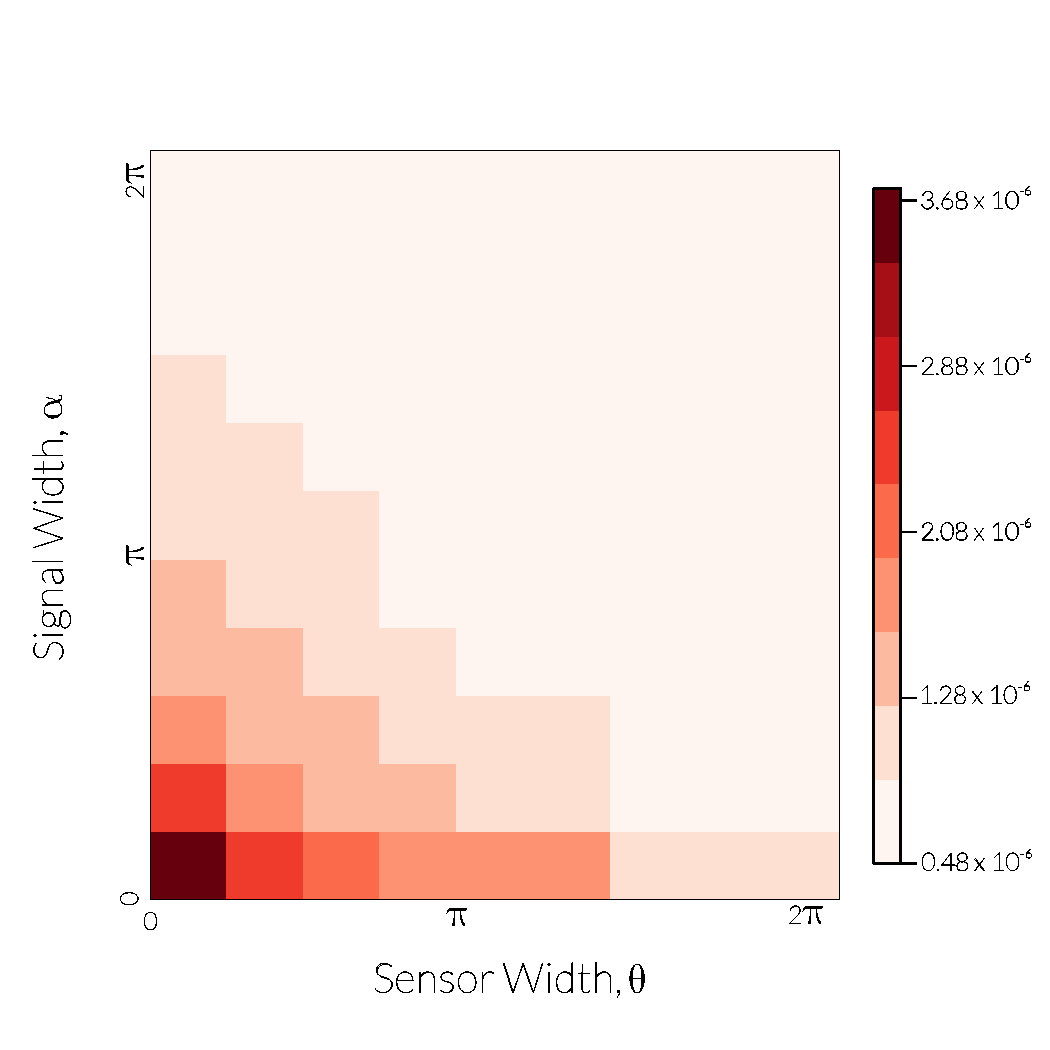
\includegraphics[width=\textwidth]{imgs/ResultStandardDeviation.pdf}
	\caption[gREM precision given a range of sensor and signal widths]{
Simulation model results of the gREM precision given a range of sensor and signal widths, shown by the standard deviation of the error between the estimated and true densities. 
Standard deviations are shown from deep red to pink, representing high to low values between $0.483\times10^{-6}$ to $3.74\times10^{-6}$. 
        } 
	\label{f:StandardDeviation}
\end{figure}


\clearpage
\section{Supplementary Information: Impact of parameter error}




\begin{figure}[h!]
  \centering
{
  \subfloat[label{f:signal}]{
    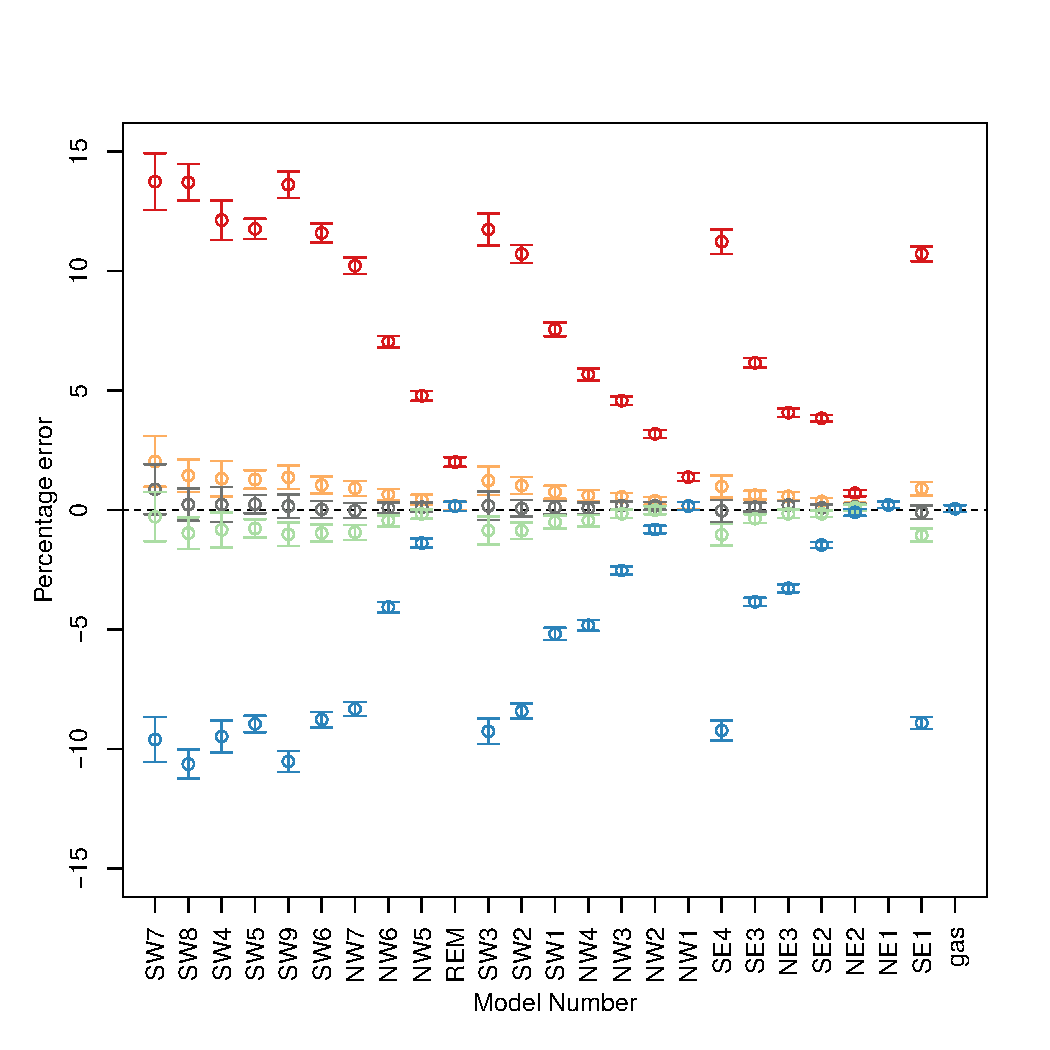
\includegraphics[width=0.4\textwidth]{imgs/AverageModelBias_callerror.pdf}
  } 
  \subfloat[label{f:sensor}]{
    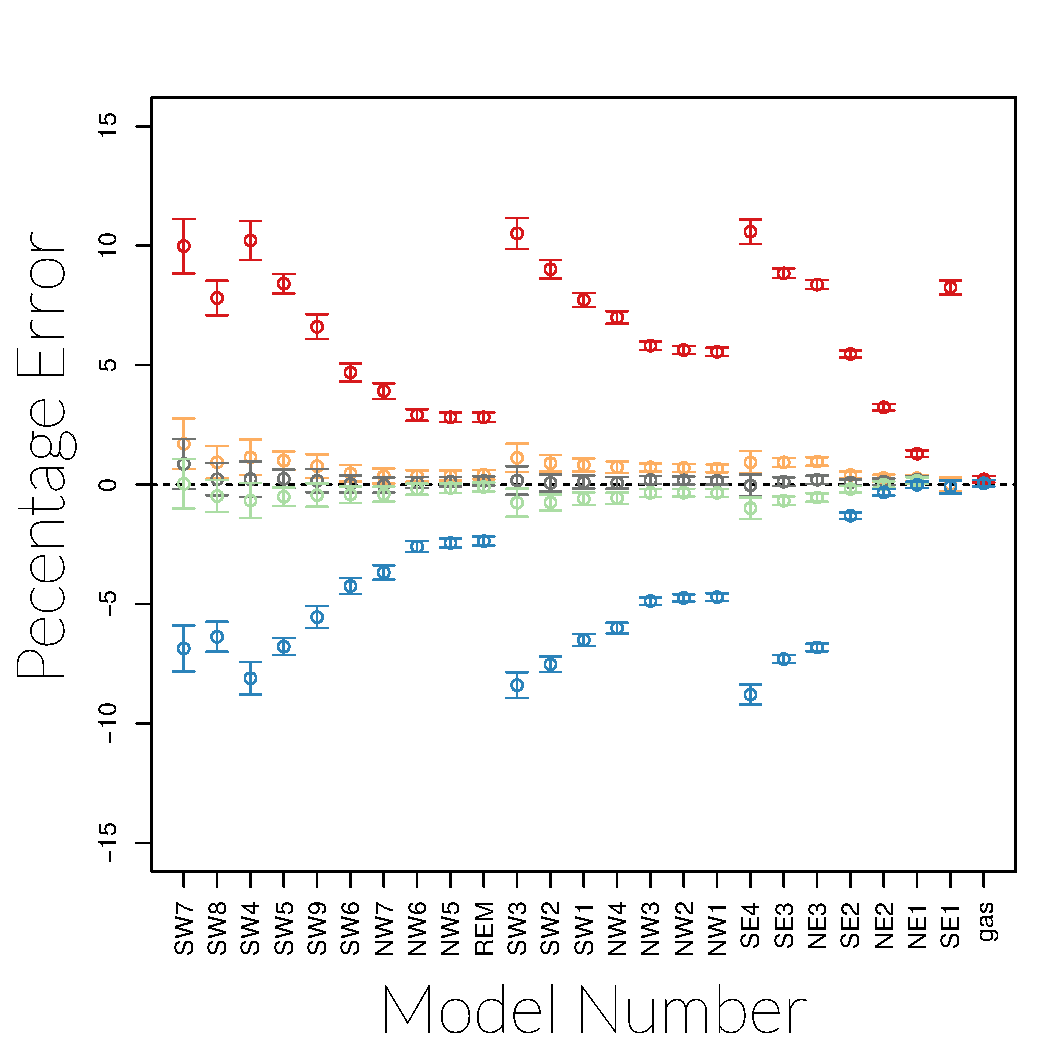
\includegraphics[width=0.4\textwidth]{imgs/AverageModelBias_cameraerror.pdf}
  } 
    
	\subfloat[label{f:radius}]{
    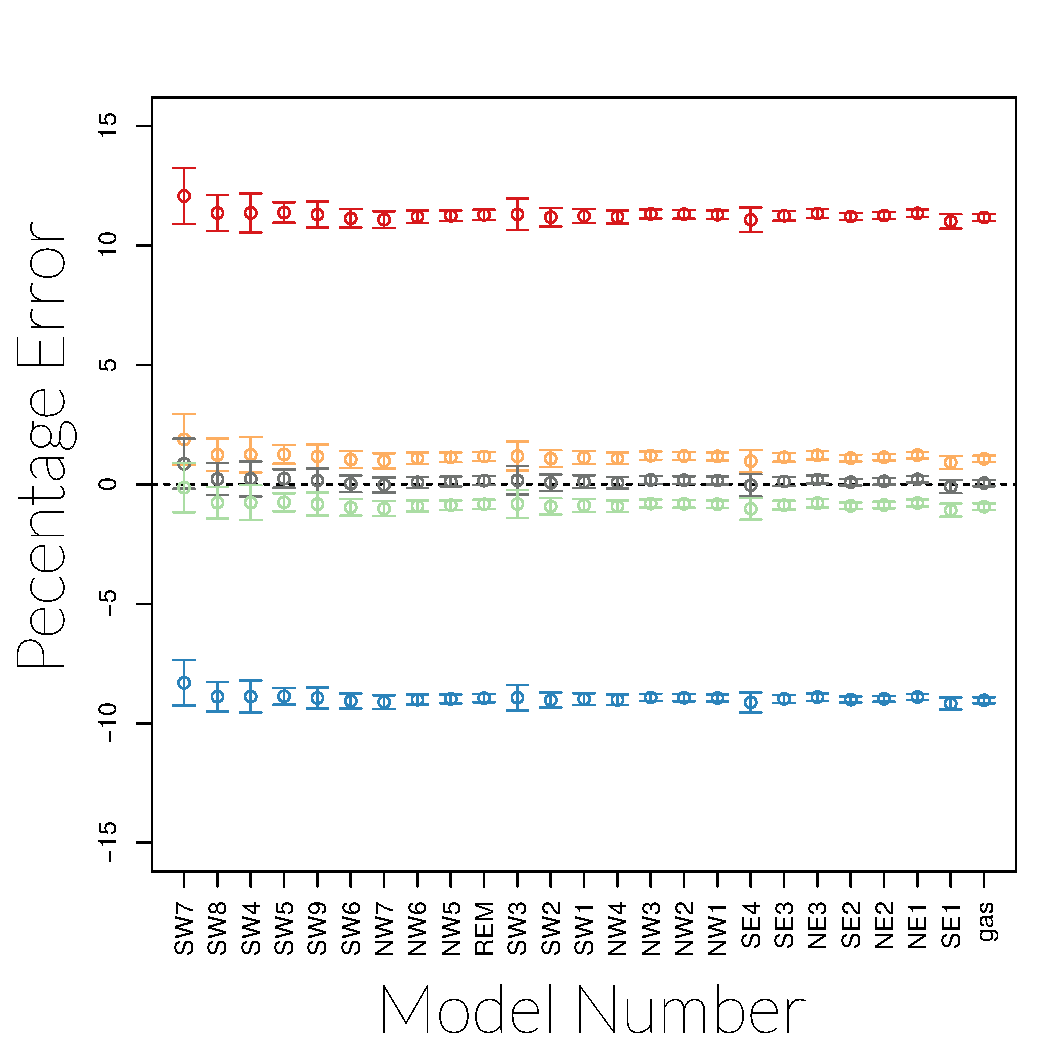
\includegraphics[width=0.4\textwidth]{imgs/AverageModelBias_radiuserror.pdf}
  }%%
	\subfloat[label{f:speed}]{
    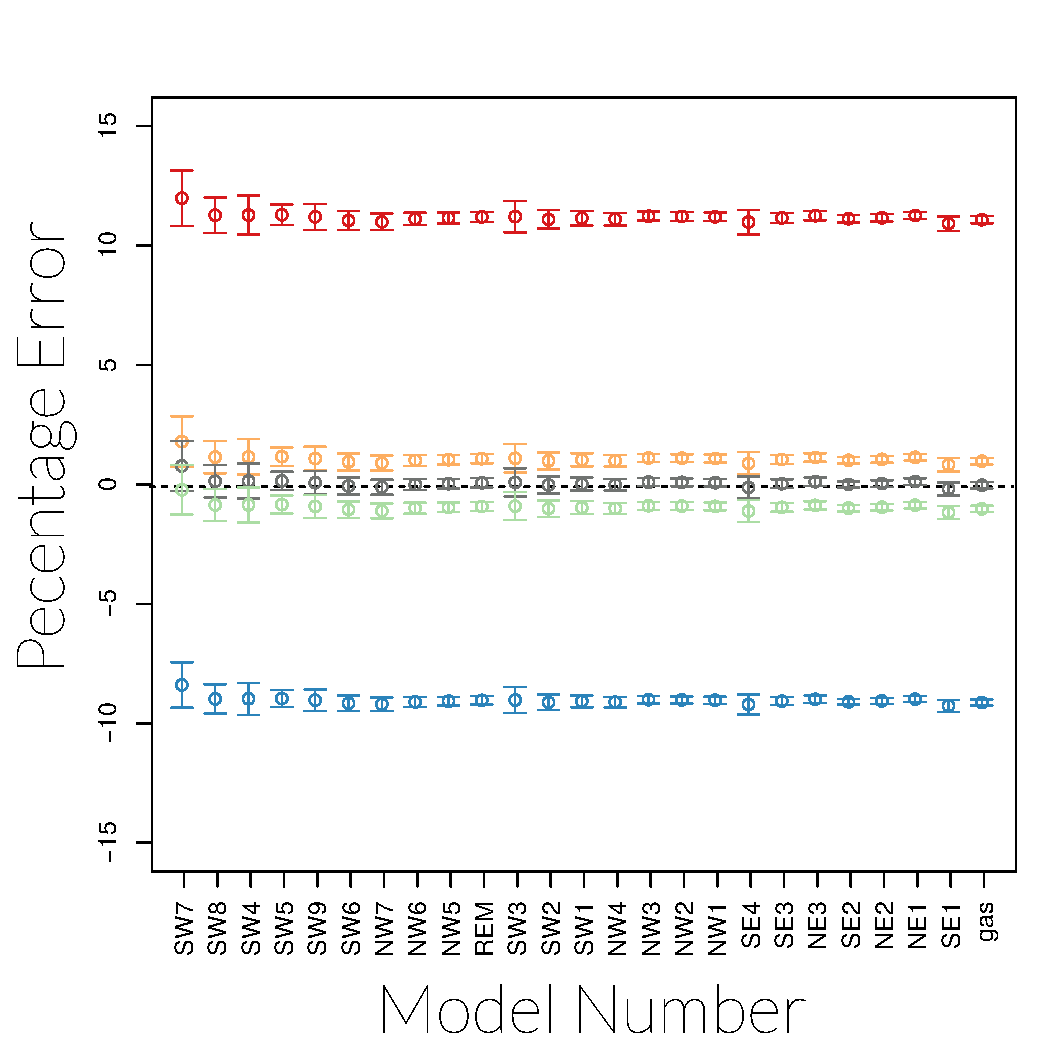
\includegraphics[width=0.4\textwidth]{imgs/AverageModelBias_speederror.pdf}
  }
}%%
\caption[Model sensitivity to error in parameter estimates]{
Model sensitivity (for all gREM submodels) to error in estimates of a) signal width $\alpha$,  b) sensor width $\theta$, c) detection distance $r$ and d) animal movement speed $v$. 
Estimates are -10\% (red), -1\% (orange), 0\% (grey), +1\% (green) and +10\% (blue) of the true parameter value. 
The black dashed line indicates zero error in density estimates. 
The error bars 95\% confidence intervals across all simulations.
}

\label{f:sensitivity}
\end{figure}








\small
\bibliographystyle{unsrt}	% (uses file "plain.bst")
\bibliography{epilit}		% expects file "myrefs.bib"


\end{document}
